\documentclass[a4paper, twoside]{report}

%% Language and font encodings
\usepackage[english]{babel}
\usepackage[utf8x]{inputenc}
\usepackage[T1]{fontenc}

%% Sets page size and margins
\usepackage[a4paper,top=3cm,bottom=2cm,left=3cm,right=3cm,marginparwidth=1.75cm]{geometry}

%% Useful packages
\usepackage{amsmath}
\usepackage{graphicx}
\setlength{\marginparwidth}{2cm}
\usepackage[colorinlistoftodos]{todonotes}
\usepackage[colorlinks=true, allcolors=blue]{hyperref}
\usepackage{graphicx}
\usepackage{tabularx} 
\usepackage{tikz}
\usetikzlibrary{arrows.meta, positioning, shapes.geometric, shadows, bending, fit, backgrounds}
\setlength{\parindent}{0pt}
\usepackage{listings}
\usepackage{xcolor}
\usepackage[most]{tcolorbox}

% Modern Code Palette
\definecolor{codebackground}{RGB}{248, 249, 250}
\definecolor{codeframe}{RGB}{220, 225, 230}
\definecolor{json_key}{RGB}{131, 37, 131}       % Purple
\definecolor{json_string}{RGB}{15, 128, 25}     % Green
\definecolor{json_number}{RGB}{0, 92, 197}      % Blue
\definecolor{json_punct}{RGB}{106, 115, 125}    % Grey

\lstdefinelanguage{json}{
    basicstyle=\small\ttfamily\color{black},
    numbers=left,
    numberstyle=\tiny\color{json_punct},
    stepnumber=1,
    numbersep=10pt,
    showstringspaces=false,
    breaklines=true,
    stringstyle=\color{json_string},
    literate=
     *{0}{{{\color{json_number}0}}}{1}
      {1}{{{\color{json_number}1}}}{1}
      {2}{{{\color{json_number}2}}}{1}
      {3}{{{\color{json_number}3}}}{1}
      {4}{{{\color{json_number}4}}}{1}
      {5}{{{\color{json_number}5}}}{1}
      {6}{{{\color{json_number}6}}}{1}
      {7}{{{\color{json_number}7}}}{1}
      {8}{{{\color{json_number}8}}}{1}
      {9}{{{\color{json_number}9}}}{1}
      {:}{{{\color{json_punct}{:}}}}{1}
      {,}{{{\color{json_punct}{,}}}}{1}
      {\{}{{{\color{json_punct}{\{}}}}{1}
      {\}}{{{\color{json_punct}{\}}}}}{1}
      {[}{{{\color{json_punct}{[}}}}{1}
      {]}{{{\color{json_punct}{]}}}}{1},
}

% Modern container for listings
\newtcolorbox{moderncode}[1][]{
    colback=codebackground,
    colframe=codeframe,
    coltitle=black,
    fonttitle=\bfseries\sffamily\small,
    boxrule=0.5pt,
    arc=4pt,
    left=15pt,
    right=5pt,
    top=5pt,
    bottom=5pt,
    before skip=10pt,
    after skip=10pt,
    #1
}

\title{M.E.R.I.T: Multi-source Employment Ranking \& Insight Tool}
\author{Rayan Akhtar}

\begin{document}
\input{title/title.tex}

\begin{abstract}
  Over the past few years, there has been a rapid increase in the number of technical roles globally, leading to intensified competition
among candidates and increasing the volume of applicants that recruiters must screen. The resulting pressure on recruiters from this
candidate pool has placed strain on Curriculum Vitae (CV) reviews. This has led to a shift towards automated screening tools to
process large batches of candidates. However, the current state-of-the-art automated screening systems remain rigid, opaque, and dependent
on the CV as a sole source of information.

This report presents \textbf{M.E.R.I.T} (Multi-source Employment Ranking \& Insight Tool), a customisable prototype multi-source
screening system designed to modernise technical recruitment by moving beyond this single-source dependency. MERIT supplements a
candidate's CV with evidence from alternative sources such as GitHub and LinkedIn, with GitHub forming the primary evaluated source in
this work. The system computes flexible metrics that are derived directly from the Job Description (JD), and provides glass-box
explanations for its candidate rankings to allow recruiters to challenge the rankings, rather than succumb to automation bias. To the
best of our knowledge, no prior published system targets technical recruitment by combining extensible JD-driven weighting, multi-source
fusion, and explainable scoring in one auditable architecture.

The system's architecture is built around three key concepts, each of which ties into the stages of a screening pipeline. The first stage
is the ingestion stage, where MERIT introduces \emph{extensible} metric extraction and weighting, providing recruiters with the tooling
to define their own priorities for a particular job. The next stage is the scoring process, where MERIT leverages \emph{multi-source}
fusion to build an in-depth profile of the candidate, highlighting any alignments or contradictions between the candidate's self-reported
information and the evidence from the alternative sources. In the last stage, recruiters would often be met with raw numbers, with no
explanation or justification for the score. Instead, MERIT explores \emph{explainable} scoring, offering transparent audit trails and
source-level attribution to allow recruiters to understand the score, as well as the reasoning behind it.

Our evaluation highlights MERIT's capacity to recover qualified candidates that are often overlooked by CV-only screening systems,
especially where self-reported CV text understates demonstrated public work, as in hidden-gem profiles where rank shifts of up to eight
places were observed once GitHub evidence was fused. MERIT's ability to separate candidates on the basis of demonstrated
evidence is also presented through a Spearman correlation of $\rho = 0.733$ between MERIT (Full) and recruiter consensus in one
high-discrimination cohort ($n = 10$, exploratory). In addition, a small-scale pilot study supports the feasibility of the system, with
evidence of recruiters reversing their decisions when presented with fraud alerts, keyword stuffing, or stronger demonstrated evidence.

MERIT is presented in this report as an \textbf{auditable screening assistant} designed with the intent of supporting recruiters in their
decision-making process, rather than a fairness-certified or fully autonomous hiring authority.

\end{abstract}

\renewcommand{\abstractname}{Acknowledgements}
\begin{abstract}
  Alhamdullilah (Praise be to God) for giving me the wisdom and motivation to see this project through to the end, and continuously refine it to ensure it is as effective as possible.

I would like to give a special thanks to my family, for their support throughout my academic journey. I would not be here without their care, support and sacrifices.

Next, I would like to thank my supervisor, Dr. Thomas Lancaster, for his support throughout my project.
I also appreciate his insights, guidance and feedback, to make this software the best that it can be.
I am also grateful to Dr. Calvin Tsay for being my personal tutor and providing me with academic advice throughout my degree.

Finally, I would like to thank my friends for their encouragement, feedback, and motivation during this project. 
Their support not only helped me stay focused but also contributed to creative discussions, including offering their thoughts on the name of this project, M.E.R.I.T., which now carries personal significance and meaning.


\end{abstract}

\tableofcontents
% \listoffigures
% \listoftables

\chapter{Introduction}

This project presents the development of \textbf{M.E.R.I.T} (Multi-source Employment Ranking \& Insight Tool), a customisable screening system designed to modernise technical recruitment by moving beyond a single-source dependency. 
While current hiring processes rely almost exclusively on the Curriculum Vitae (CV), MERIT integrates observable evidence from multiple data streams to provide a more thorough evaluation of a candidate’s technical competencies. 
By supplementing the CV with external sources such as GitHub and LinkedIn, the tool aims to capture a candidate’s true technical proficiency, rather than relying solely on the self-reported skills present in the CV (which may be referred to as a resume in other regions).
\\\\
Over the past few years, there has been a rapid increase in the number of technical roles globally, leading to intensified competition among candidates and increasing the volume of applicants that hiring managers must screen. 
Organisations often attempt to streamline early-stage screening by requiring concise CV formats. 
While the one-page resume is standard in the US as well as entry-level roles, UK standards often allow for two pages, particularly in more experienced, technical roles. 
Regardless of the length requirement imposed, decades of research in personnel selection highlights that CV-based screening is cognitively demanding for these recruiters, and also highly vulnerable to bias \cite{moore2023}. 
Since CV reviews require rapid judgments under relatively tight time constraints with limited information, evaluators often rely on heuristics rather than a systemic assessment of actual job-relevant qualifications \cite{tversky1974}.
\\\\
Rapid manual screening often amplifies cognitive biases, such as contrast effects, where a candidate's evaluation depends on the relative quality of preceding candidates \cite{palmer2014}. 
These biases are significantly worse in technical recruitment, where skills are harder to assess, leaving evaluators to rely on superficial cues. 
CV information itself is also unreliable: candidates may exaggerate responsibilities, or omit weaker experiences \cite{birkeland2006_applicant_faking_behavior}, tend to overestimate competencies, particularly in programming \cite{dunning2004}, and technical skills may decay overtime if left unused \cite{arthur1998}. 
Collectively, these factors reduce the reliability of manual CV assessments.
\\\\
To address these challenges, many organisations adopt automated or semi-automated screening systems, which usually rank candidates based on keywords, education and work experience to generate a pass/fail score. 
These systems reduce workload and speeds up the hiring process, however, it does introduce limitations. 
They often ignore “new talent signals”, such as project portfolios, open-source contributions, or other verifiable demonstrations of ability, which can provide a better assessment of technical skills \cite{chamorro2016}. 
By overlooking “new talent signals” and relying on rigid scoring frameworks, automated systems underestimate qualified candidates and reinforces a narrow, one-size-fits-all approach. 
There is also a lack of transparency for screening systems, leaving recruiters with limited insight into why candidates pass or fail the process.
This `black-box' nature reduces trust and makes it difficult for hiring managers to verify the fairness of the automated decision \cite{raghavan2020}.
\\\\
Automated systems are also shown to inherit biases present in past hiring data. 
Gender, ethnicity, and institutional prestige can influence a model's output, reproducing the discrimination present in manual screening processes \cite{raghavan2020,bogen2018}. 
Also, relying solely on CV data prevents the verification of self-reported skills and fails account for skill decay, which is especially important in technical domains where competencies evolve rapidly \cite{arthur1998}. 
As well as that, most tools lack flexibility, applying identical scoring frameworks to all candidates and limiting recruiters' ability to prioritise role-specific competencies \cite{chamorro2016}. 
\\\\
These gaps highlight the need for adaptable, explainable, and multimodal approaches that are capable of assessing both the technical and behavioural skills while mitigating bias. 
High-validity selection methods are shown to improve an employee’s performance and productivity, leading to measurable economic and organisational benefits \cite{schmidt1998}. 
An accurate early-stage screening process is therefore critical to reduce the likelihood of a bad hire.
\\\\
MERIT addresses these issues through the combination of traditional CV data with verified behavioural and proficiency-based evidence from multiple sources, such as GitHub and LinkedIn. 
By focusing on observable performance and providing transparent, explainable justifications for its rankings, MERIT aims to reduce bias, improve reliability, and aid evidence-based decision-making in technical recruitment.


% \section{Contributions}
% MERIT takes inspiration from most existing implementations of screening systems commonly found both in academia, as well as in the industry, notably systems that take CV information along with a job description to decide on whether to progress a candidate to the next stage. 
% However, this paper introduces the following novel contributions:

% \begin{enumerate}
%   \item \textbf{Multimodal Data Integration:} By integrating data from various data sources (such as GitHub, LinkedIn and CVs), the system aims to get a better understanding of a candidate's abilities, beyond the single page CV submitted. 
%   This addresses the issue of limited CV information, allowing for a better evaluation of technical and non-technical skills.
  
%   \item \textbf{Inferred and Customisable candidate evaluation:} This system will have the ability to optionally anonymise a candidate's data, and standardise CV formats to remove biases on gender, ethnicity and visual presentation. 
%   This will tackle the issue of biases with regards to the format of a CV and company names to ensure a fairer recruitment process.
  
%   \item \textbf{Explainable AI and report customisation:} Candidate evaluation metrics are to be automatically inferred from the job description, whilst also allowing recruiters to customise these for more precise assessments. 
%   Recruiters will also be able to adjust the strength for ranking metrics to address the rigid one-size-fits-all approach present in most automated screening systems. 
%   This allows recruiters to prioritise the factors that matter most for their role and organisation.
  
%   \item \textbf{Bias Mitigation:} Clear explanations will be expected for candidate scoring, and there will be both short summaries, as well as detailed reports to ensure transparency in the evaluation process. 
%   This will allow recruiters to understand the rankings behind a candidate, to better inform them in these data-driven hiring decisions. 
%   Reporting will also need to clarify the data source for which this evidence was derived from to ensure fairness and transparency once again. 
%   A candidate's key strengths and weaknesses will also be highlighted on their profile, and comparisons will be made against other candidates who also possess these metrics.
  
%   \item \textbf{Interview Preparation Insights:} Weak or unknown metrics on a candidate profile will be flagged, and suitable interview questions will be suggested to address these gaps in candidate area, or in areas of high uncertainty. 
%   For missing data sources, the system can be configured to automatically email candidates for missing data to prevent candidate's from being disadvantaged should the system not be able to extract this information from their CV.
% \end{enumerate}

% By combining these contributions together, MERIT can:
% \begin{enumerate}
%   \item Provide a fairer and more accurate assessment of the candidate's abilities, reducing the ability for candidates to overestimate their abilities.
  
%   \item Eliminate discrimination and contrast-related biases from hiring managers.
  
%   \item Provide transparency on automated screening through detailed reporting, rather than numerical scores, or surface level reasoning.
% \end{enumerate}
\chapter{The Current State of Technical Recruitment}

This chapter examines the operational framework of modern technical hiring to identify the systemic inefficiencies that necessitate a multimodal screening approach.
The chapter begins by exploring the diversities inherent in technical roles as well as the limitations of job descriptions as a formal, yet inconsistent, role specification.
Following this, the chapter outlines the standard multi-stage recruitment process pipeline and evaluates the various data sources that are typically leveraged during candidate screening.
The discussion concludes by investigating traditional manual screening, as well as the specific challenges faced due to various cognitive biases as well as fatigue.
By establishing these foundational elements, this chapter demonstrates that a reliance on the Curriculum Vitae as a single source of truth is insufficient for technical selection.
This identifies a critical need for automated solutions, and the technical frameworks explored in the subsequent chapter ultimately justify the need for MERIT as a multi-source solution for verifiable candidate assessment.

\section{Technical Roles}

Technical roles refer to those within the technology sector. They often vary in terms of the competencies required and
also span many different domains, from full-stack development to cloud infrastructure management, to machine learning.
In most cases, these roles are listed under generic titles, such as ``Software Engineer'', while the competency and seniority
for the role differ drastically between vacancies. Due to this, it is likely that candidates from adjacent domains may
apply for the same role, even if they are not a good fit. This ambiguity warrants a job description to specify the
competencies and seniority expected for each vacancy.

\section{Job Description}

A job description (JD) is a document that outlines the purpose of a role, as well as the competencies required.
In the technical landscape, requirements are usually explicitly listed, such as programming languages, frameworks,
tooling, seniority and responsibilities. Hiring managers use this text to decide which skills to prioritise,
and to what extent each of these should influence shortlisting, however, most JDs are written for candidates,
not for machines. As such, there is often prose that is not relevant to the screening process, such as benefits and company culture.

There is currently no industry standard for JDs, hence they differ in terms of clarity and depth.
Some postings detail requirements precisely, while others follow boilerplate text that repeats common terms across roles.
Candidates often form unrealistic expectations due to this lack of clarity and specificity \cite{breaugh1983,earnest2011}. 

Regardless, in most cases, the JD can be seen as a valuable source of information for the screening process, given that
the system is able to separate the requirements from the prose. Many screening systems do not take advantage of this, instead
applying fixed weights and metrics to measure against, even when the JD may vary in terms of stack and seniority level~\cite{gugnani2020,lo2025aihiring}.
A screening system that is not tailored to a specific JD is likely to be generic, and may pick the best ``average'' candidate,
rather than the best candidate for that specific role. Given this, rigid scoring systems may miss strong candidates, and
shortlist candidates that are not a good fit for the role when the screening configuration does not reflect the JD~\cite{fuller2021hiddenworkers}

MERIT must, therefore, treat the JD as a noisy configuration document, separating explicit requirements from redundant
information. It extracts listed technical metrics and suggests relative weights via corpus-aware TF-IDF, which recruiters
can add to, remove or override before scoring.

\section{Recruitment Process Pipeline}

Figure~\ref{fig:tech-recruitment-pipeline} summarises a typical technical hiring pipeline.
Solid boxes denote core stages; dashed boxes are optional or organisation-dependent (more common in larger firms with the resources to run them).
The job offer is visually distinguished from intermediate stages.

\begin{figure}[htbp]
\centering
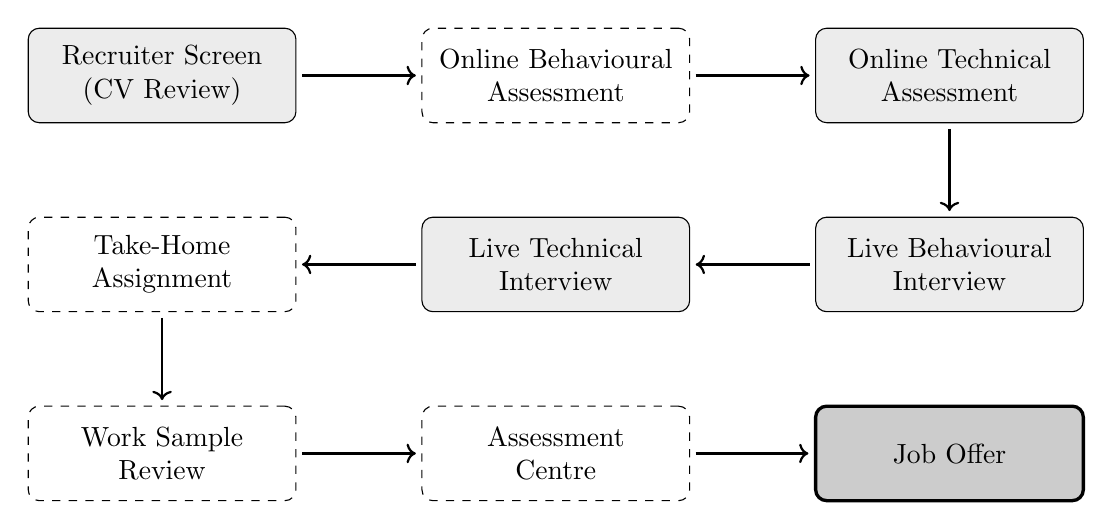
\begin{tikzpicture}[
    box/.style={
        draw,
        rectangle,
        rounded corners,
        align=center,
        minimum height=1.2cm,
        minimum width=3.4cm
    },
    core/.style={box, fill=gray!15},
    optional/.style={box, dashed},
    outcome/.style={
        box,
        fill=gray!40,
        draw=black,
        line width=1.2pt
    },
    arrow/.style={->, thick, shorten >=2pt, shorten <=2pt}
]

% ===== Row 1 =====
\node[core]     (cv)   at (0,0)   {Recruiter Screen\\(CV Review)};
\node[optional] (beh)  at (5,0)   {Online Behavioural\\Assessment};
\node[core]     (oa)   at (10,0)  {Online Technical\\Assessment};

% ===== Row 2 =====
\node[optional] (takehome) at (0,-2.4) {Take-Home\\Assignment};
\node[core] (techint) at (5,-2.4) {Live Technical\\Interview};
\node[core]     (live) at (10,-2.4) {Live Behavioural\\Interview};

% ===== Row 3 =====
\node[optional] (ac)    at (0,-4.8) {Work Sample\\Review};
\node[optional] (behint) at (5,-4.8) {Assessment\\Centre};
\node[outcome]  (offer) at (10,-4.8) {Job Offer};

% ===== Row 1 Arrows =====
\draw[arrow] (cv.east) -- (beh.west);
\draw[arrow] (beh.east) -- (oa.west);
\draw[arrow] (oa.south) -- (live.north);

% ===== Row 2 Arrows =====
\draw[arrow] (live.west) -- (techint.east);
\draw[arrow] (techint.west) -- (takehome.east);
\draw[arrow] (takehome.south) -- (ac.north);


% ===== Row 3 Arrows =====
\draw[arrow] (ac.east) -- (behint.west);
\draw[arrow] (behint.east) -- (offer.west);

\end{tikzpicture}
\caption[Technical recruitment pipeline]{Typical technical recruitment pipeline (core vs.\ optional stages).}
\label{fig:tech-recruitment-pipeline}
\end{figure}

When it comes to the application for technical positions, candidates will typically progress through multiple evaluation stages. 
While the sequence and steps taken often vary due to organisation size and maturity, industry research consistently shows that the technical recruitment pipelines will follow a multi-step structure \cite{cappelli2019}. 


\subsubsection{Recruiter Screen}
The hiring process for most organisations often starts off with a brief review of a candidate's CV to filter out 
candidates that are not suitable for the role. This is often performed by a recruiter or a hiring manager.
There has been a recent shift towards AI-driven pre-screening due to the rise in candidate applications, this
pre-screen is aimed to reduce the number of candidates that even make it to the first human review stage of the hiring process.
This significantly reduces applicant volumes, allowing for a more focused screening process, however, it is often at the cost
of algorithmic bias and opaque decision-making being introduced into the process.

Regardless of whether the process is a screen or a pre-screen, the CV itself is still the primary document evaluated.
However, industry research suggests that companies are becoming dissatisfied with typical CV data, such as past job titles
and educational prestige, when it comes to technical recruitment. It is noted that the industry is shifting towards skill-based
assessments to verify a candidate's competencies \cite{hackerrank2024skills}. Candidates are encouraged to provide their
GitHub URL as part of their application, however, research shows that this data is often reviewed inconsistently
during early stages, instead relying mainly on CVs as opposed to external behaviour evidence \cite{moore2023}.

\subsubsection{Online Behavioural Assessment} 
Larger enterprises commonly have an additional behavioural assessment, often in the form of a game, or a recorded interview, where candidates are prompted to record their response to common interview questions. 
Increasingly, these asynchronous video interviews are being augmented or fully driven by AI. Platforms employing machine learning 
algorithms can analyse a candidate's tone of voice, facial expressions, pacing, and keyword usage to algorithmically assess their 
personality and cultural fit. 
These tools, while uncommon in typical technical hiring pipelines, are more established in large-enterprise pre-screening: 
among Fortune 500 firms, 20\% already use asynchronous pre-recorded video interviews, with a further 17\% planning to adopt 
them, assessing dimensions such as communication style that are difficult to infer from a CV alone \cite{ithaka2018_assessment}. 
Smaller companies, however, rarely adopt such methods due to cost, limited perceived value and candidate-dropout risk.

\subsubsection{Online Technical Assessment}
Online technical assessments (commonly referred to as OAs) are core to the hiring process for many organisations. 
OAs often take place on platforms such as HackerRank and CodeSignal, and often focus on Data Structures and Algorithms (DSA). 
Industry surveys show that online technical assessments remain central to hiring pipelines: CoderPad's 2025 survey reports 
that 24.5\% of employers use asynchronous technical tests and 49.8\% use live coding interviews \cite{coderpad2025techhiring}, 
and CodeSignal highlights continued growth in standardised early-stage technical evaluations \cite{codesignal2023}.

\subsubsection{Live Behavioural Interview}
Live behavioural interviews are a common stage in technical recruitment, often conducted by HR or hiring managers to assess a candidate's cultural fit, communication skills and motivations for the role and company.
This process follows traditional interview formats, with a focus on behavioural questions alongside further discussions regarding the candidate's background, providing a better insight into a candidate's previous experiences and soft skills.

\subsubsection{Live Technical Interview}
Live technical interviews refer to the group of assessments which often involve an element of programming in front of an engineer at the hiring organisation, often involving live-coding, pair programming, or on-the-spot problem solving. 
These forms of assessment remain as a core part of the process for most software engineering hiring processes when it comes to evaluating a candidate's technical proficiency. 
As such, many organisations treat this as a central evaluation stage. 
While reliable aggregate data for this is scarce, multiple industry-level reports and practitioner accounts can confirm that live technical interviews remain an essential method for assessing candidates \cite{karat2020}. 

Some academic and industry critiques point out the limitations of this format, specifically stress under observation, lack of realism, and poor predictive validity for long-term developer performance. 
This suggests that hiring pipelines should leverage alternative assessment methods as opposed to solely live coding rounds \cite{behroozi2019hiring}.

\subsubsection{Take Home Assignment}
For organisations that prefer “skill-based hiring”, they may incorporate take-home tests as part of their technical hiring process. 
These assignments require a candidate to build or extend a small system, followed by a review interview. 
According to TestGorilla's 2024 survey, a large portion of employers report using assignment, or work-sample based assessments as a part of their hiring pipeline, highlighting the relevance of take-home assessments for a realistic evaluation of coding ability and design choices \cite{testgorilla2024}. 
They argue that these assignments provide a better benchmark for the candidate's real-world development skills rather than time-limited algorithmic tests and whiteboard interviews.

\subsubsection{Work Sample Review}
Many employers like to also use real-world evidence, such as GitHub repositories, open-source commits and portfolio projects to assess a candidate's ability to build software. 
This data is often a critical differentiator, as it is able to separate a candidate's claims from their actual abilities.
Historical data highlight that the majority of firms (80\% of small and 66\% of large firms) place high value on portfolio evidence,
such as GitHub \cite{hackerrank2018skills}. Recent reports also come to a similar conclusion, that verified technical 
assessments are essential in addressing the limitations of traditional CVs \cite{hackerrank2024skills}.
However, this is often done later in the pipeline due to the time and expertise required for evaluation. 
Academic literature shows that work-sample tests are one of the highest-validity predictors of job performance (validity coefficient of 0.54) \cite{schmidt1998}, significantly outperforming CV-based assessments.

\subsubsection{Assessment Centre}
An assessment centre (commonly referred to as AC) is a structured multi-exercise evaluation process, often used in graduate programs and enterprise-level hiring. 
Recent UK survey data suggest that a minority of organisations (32\% in 2020) use formal assessment centres as part of their selection process \cite{cipd2020_resourcing}. 
Where assessment centres are used, UK employers commonly apply methods such as group exercises, psychometric tests, role plays and combined tasks to evaluate teamwork, communication and problem-solving \cite{cipd2022}. 
While not widely used, ACs remain useful for gaining deeper insights into the candidate's interpersonal and non-technical capabilities.

\subsubsection{Relevance to MERIT}
Given the complexities and inconsistencies that are present in the technical hiring process, the screening stage remains to be the most influential, yet error prone point in the process. 
Organisations rely heavily on this filter, yet early decisions are often solely based on a brief CV review, which is often shown to be vulnerable to bias, information loss and unreliable judgement. 
MERIT will target this part of the pipeline to improve accuracy, fairness and evidence-quality in order to produce the greatest organisational impact.

MERIT will strengthen screening through the integration of multi-source evidence, such as GitHub activity, CV data, and other sources, to provide verifiable behavioural and technical indicators. 
This early-stage assessment can reduce or refine the need for later steps, such as online coding tests, manual work-sample reviews, and broad behavioural screens, while still highlighting areas where further evaluation is necessary. 
The system will be designed to be adaptable across different organisation sizes, for example smaller firms will benefit from reduced reliance on time-consuming take-home tasks, and larger firms can improve their structured assessments with transparent data-driven insights. 
By transforming the earliest decision point into a more reliable and insightful stage, MERIT helps to create a fairer, more consistent and efficient technical hiring process.


\section{Data Sources}
\label{sec:data-sources}
Technical recruitment often requires multiple data sources to be provided to evaluate candidates beyond traditional CVs, but these are rarely used in practice. These sources have the potential to provide insights into the extensive professional history, technical competencies, behavioural tendencies as well as real-world coding practices. Effective multi-source screening will require a deeper understanding of the strengths and limitations of these data channels.


\begin{table}[htbp]
    \centering
    \caption[Overview of supplementary recruitment data sources]{An overview of supplementary data sources, their value to technical recruitment, and their inclusion in MERIT.}
    \label{tab:data-sources}
    \small
    \renewcommand{\arraystretch}{1.4}
    \begin{tabularx}{\textwidth}{>{\raggedright\arraybackslash\bfseries}p{2.6cm} >{\raggedright\arraybackslash}p{3.2cm} >{\raggedright\arraybackslash}X >{\centering\arraybackslash}p{1.5cm}}
        \hline
        \textbf{Data Source} & \textbf{Primary Function} & \textbf{Value to Technical Recruitment} & \textbf{Included?} \\ \hline
        Curriculum Vitae (CV) & Self-reported professional summary & Baseline for initial screening. Highly vulnerable to embellishment and self-report bias \cite{henle2019_resume_fraud,dunning2004}. & Yes \\
        GitHub & Version-controlled code repositories & Richest source of verifiable work-sample evidence. Demonstrates tech stack usage and coding style \cite{hackerrank2018skills,hackerrank2024skills}. & Yes \\
        LinkedIn & Professional identity and networking & Expands upon CV details. Used by 72\% of recruiters \cite{jobvite2020}. & Yes \\
        LeetCode \& HackerRank & Algorithmic practice and live assessments & Demonstrates tested technical ability and problem-solving under constraints \cite{coderpad2025techhiring}. & No \\
        Stack Overflow & Software engineering Q\&A exchange & Highlights communication style, community engagement, and domain specialisation \cite{vasilescu2013}. & No \\
        Social Media & General personal networking & Used for background checks to identify ``red flags'' \cite{careerbuilder2017_social}. High risk of bias (Note: excludes LinkedIn). & No \\ \hline
    \end{tabularx}
\end{table}

\subsubsection{Relevance to MERIT}
As shown above, there are a variety of external data sources that can be used to evaluate a candidate's suitability for a technical role
beyond the traditional Curriculum Vitae (CV). Being able to capture and integrate multiple data sources can help provide more factors
to differentiate between candidates, allowing for a more comprehensive view of a candidate's suitability for a role. MERIT aims to 
integrate GitHub as a supplementary data source due to it serving as a strong indicator of a candidate's technical ability. LinkedIn
will also be selected as a strong indicator of a candidate's professional experience and also to account for errors in the CV parsing process.
Other data sources such as LeetCode and HackerRank are likely to not be selected as supplementary data sources due to the time 
constraints during development, however, they are still considered as potential future data sources for MERIT.




\section{Manual Screening}
In smaller organisations, early-stage screening is still likely to be manually conducted, 
due to the cost of implementing and maintaining an automated screening system.
Recruiters and hiring managers will usually review a candidate's CV, along 
with application data, to compare against the job description to determine 
whether the applicant meets the minimum experience and skill requirements.
The screening stage is designed not to find the best candidate, 
but to instead to reject candidates that are considered unsuitable for the role, 
allowing for a more focused and efficient interview process.
In order to manage large applicant pools, recruiters may also introduce 
implicit filtering criteria in an attempt to simply reduce the number of 
candidates progressing into more resource-intensive interview stages.
While manual screening can be effective in recruitment, it often suffers 
from a range of limitations and biases that can reduce the overall quality, 
fairness and consistency of the process.

A primary issue revolves around biases due to time pressure and superficial 
evaluation, as recruiters usually spend little time on a first-pass, leading 
to them overlooking critical information.
The issues are further exacerbated by information overload and cognitive load 
bias, where excessive information leads to increased decision difficulties as 
well as a reliance on cognitive shortcuts rather than careful evaluation, as shown in research on information overload \cite{che2019}.
Furthermore, the repetitive task and fatigue effect suggests that when recruiters 
process multiple candidates in a session, their decision quality degrades.
This is supported by a PNAS study from Danziger et al., which highlights that favourable rulings drop 
sharply as decision-makers process more cases without breaks \cite{danziger2011}. 
Note that this work studied judicial parole decisions rather than hiring, but the same fatigue pattern may also apply to high-volume CV screening.
The mood and emotional state bias causes further issues as the Affect Infusion 
Model indicates that a recruiter's emotional state under stress can lead to a change 
in their perception or judgement of a candidate's suitability for that role \cite{forgas1995}.

Beyond these operational constraints, the screening process is also influenced by 
other distortions that introduce further bias.
The determinism of the recruitment process is affected by the contrast effect, as 
candidate evaluation may be unfairly affected by the quality of candidates that precede 
them \cite{palmer2014}.
This issue is made worse with the anchoring bias, where they over-rely on the first 
piece of information encountered, such as a previous employer or job title, which then 
disproportionately influences the rest of the screening \cite{buijsrogge2021}.
Halo and horn effects also tie in closely to this, where a recruiter generalises from 
one positive or negative attribute, such as a prestigious company, or a single typo, to 
the entire candidate profile \cite{thorndike1920}.
The previously mentioned issues are further worsened due to imperfect and exaggerated 
self-reported information where candidates may embellish or misrepresent their skills and 
experiences to appear more favourable \cite{dunning2004}.

Finally, manual screening is also vulnerable to systemic discrimination and group-based preferences.
For instance, field experiments by Bertrand and Mullainathan found that name 
and ethnic discrimination plays a key issue.
This is shown through their findings where “white sounding” names received around 
50\% more callbacks compared to “African American sounding” names despite identical qualifications \cite{bertrand2004}.
The main cause of this often comes down to similarity bias and in-group bias. This is the idea that
individuals tend to favour applicants who resemble them, often in terms of factors such as background, nationality
and educational route \cite{tajfel1986}.


The core limitations, as shown above, come down to time pressure, cognitive load, and applicant volume. 
The biases mentioned uncover the unfairness behind manual screening, more specifically the lack of consistency
and objectivity in this process.
As more candidates enter the application process, these psychological and procedural 
limitations compound further, leading to inconsistent outcomes, reduced fairness and 
also the potential for a poor selection quality.
Such challenges highlight the need for a more reliable, systematic and transparent 
screening method, more specifically automated, data-driven systems that are able to 
evaluate a candidate against a job requirement with better consistency, scalability, 
and a reduced vulnerability towards any potential human bias.


\chapter{Related Work \& Technical Foundations}

After gaining an understanding of the cognitive limitations and biases present in traditional technical recruitment,
we now turn towards the frameworks designed to automate candidate evaluation.
The chapter first categorises the various Applicant Tracking Systems (ATS) based on the logic of their scoring
engines. From here, we review prior work thematically across the three strands that can map to the limitations that MERIT
is designed to solve. We cover the ideas of extensibility (Section~\ref{sec:lit-extensibility}), 
multi-source verification (Section~\ref{sec:lit-multi-source}), 
and transparency and explainability (Section~\ref{sec:lit-transparency}).
The ideas also cover important technical foundations that will be used to support our design ideas in
Chapter~\ref{ch:implementation}. Finally, the chapter closes with
an overview, summarising how these three areas motivate MERIT~\cite{merit_repo}.

\section{Automated Screening}
\label{sec:automated-screening}

Organisations often rely on automated screening systems to filter, rank or manage large volumes of candidates.
These screening systems may also be referred to as Applicant Tracking Systems (ATS) throughout the rest of this report
for brevity. According to Jobscan's 2022 entry, we have that 97\% of large firms leverage these ATS platforms.
While there are no statistics on the adoption of small to medium-sized firms, it is reasonable to assume that
most organisations use ATS platforms to some extent due to the scalability and efficiency benefits they provide.

ATS platforms can be categorised in various ways, but in our report we will categorise them based on the underlying
logic of the scoring system. More specifically, we have Rule-Based, Keyword-Matching, and AI-Assisted ATS.

\subsection{Rule-Based ATS}
Rule-Based ATS systems refer to platforms that focus on explicit, pre-defined rules or criteria in order to 
screen candidates. Recruiters often configure such systems with keyword lists, required thresholds for
skills, education and experience, and other boolean queries. As such, these systems are knockout in
nature. Either a candidate satisfies every rule, or they are filtered out. It is important to note that
such systems do not provide a match score, nor do they rank candidates, instead recruiters are presented with
pass/fail shortlists. Due to their consistency and predictability, employers may leverage rule-based systems to screen candidates. 
By applying explicit, pre-defined criteria uniformly, such systems avoid the intuitive, subjective judgments that 
often influence human reviewers \cite{highhouse2008stubborn}.

The reason these systems are not commonly used however, is due to the limit of standardisation of CV formats.
These systems will struggle with non-standard CV formats, leading to parsing errors \cite{emnlp2025resumebench}.
Candidates with unconventional layouts or career paths are therefore more likely to be scored poorly for formatting 
reasons rather than skill.
Along with this, these systems are vulnerable to keyword-gaming, a practice where applicants strategically insert 
repeated or irrelevant terms to artificially inflate their match scores, a practice that is widely discussed in practitioner advice on optimising CVs for ATS parsers \cite{marr2019}.
The failure to recognise all possible CV formats and lack of semantic understanding also leads to the system being unable
to recognise unconventional experience. It may also perform poorly when skills are also presented in non-traditional ways, or
demonstrated in another section, such as open-source contributions or bootcamp projects. Rule-based systems are likely not 
exhaustive enough in the treatment of CVs and will likely score non-traditional CVs poorly, not due to the candidate's skills,
but instead due to the system's inability to recognise the candidate's skills.


\subsection{Keyword-Matching ATS}
This version of ATS is a middle ground between the previously mentioned rule-based approach, and the upcoming AI-driven version.
This form relies heavily on exact keyword matching and basic tokenisation. While some commercial versions may incorporate basic 
NLP-based parsing to recognise simple linguistic variations, such as standardising acronyms, they still offer limited
semantic understanding. They act more as advanced string-matching systems rather than engines that can understand the 
context of a candidate's experience.
Unlike rule-based knockouts, these systems typically assign match scores and rank candidates across the applicant pool rather than returning pass/fail shortlists alone.

Their strengths are mainly that they are simpler to implement and offer an increase in the transparency of the system compared 
to AI-driven systems, since much of the logic is still tied to explicit keyword counts.

Due to the simplicity of the system, it is often subject to misinterpretation issues, often failing to recognise
contextual details and ambiguous language within a CV. They also may overlook crucial nuances such as depth of skill,
quality of experience and also evidence of measurable achievement.
The misinterpretation then leads to misclassification. This is backed by employer surveys which report that more than 
90\% of employers use applicant-tracking or recruitment-management systems to filter or rank candidates, and 88--94\% 
of them believe that qualified applicants are screened out when they fail to match job-description criteria 
exactly \cite{fuller2021hiddenworkers}.

\subsection{AI-Assisted ATS}
AI-Assisted ATS comprise machine learning models, often leveraging transformers and Large Language Models (LLMs), 
to predict candidate-job fit. The system does not follow that of its predecessors, instead inferring semantic 
relationships between skills, roles and qualifications. Furthermore, many commercial versions will train on previous 
hiring data to learn which traits led to successful hires in the past.
Like keyword-matching ATS, they score and rank candidates across the applicant pool rather than applying knockout filters alone.

Due to this, the systems employ vector-embeddings and semantic search to evaluate whether a candidate is a strong 
match for the job description, or whether they are similar to other successful candidates for that role. They also take advantage
of predictive scoring models that learn from recruiter usage patterns to refine the scoring system,
picking up on hidden non-obvious signals that may be missed by traditional keyword-matching systems.

Given that the underlying system is well-trained, the key strength of AI-Assisted ATS lies in their
matchmaking accuracy, as well as detection of transferable skills. They are also able to handle 
a wider range of career paths compared to rule-based systems.

As mentioned before, the systems train on both historical hiring data and recruiter usage patterns.
This leads to a major flaw in these systems, the potential to reinforce historical biases.
Algorithmic bias is a concept where models inherit preference towards certain patterns, in this case,
it would be gender, ethnic or institutional preference found in the past hiring data \cite{raghavan2020,bogen2018}.
The potential for further discrimination is also present due to the feedback loop from recruiter interactions
if these employers continue to favour candidates with these specific traits.

Furthermore, the “black box” nature of these systems leads to low transparency, as there 
is often little explanation for ranking and rejecting decisions, undermining both 
candidate trust as well as compliance with fair-hiring guidelines.
Another significant issue lies in over-generalisation, where these models are often 
trained on broad datasets, prioritising generic markers over role-specific expertise.
In a similar fashion, domain drift also plays a role, where the system continues to 
optimise for outdated historical traits despite a company's technological or strategic shifts.

\vspace{1em}
Throughout this section, we have considered the different strengths and weaknesses of these ATS platforms, however,
there is still one major flaw that has not been discussed. This is the exclusive reliance on the candidate CV, 
completely disregarding all other sources of evidence that are typically provided by candidates (primarily GitHub and LinkedIn).
These systems work on a small subset of the data that is actually available to them, limiting their ability to truly capture
the strengths and weaknesses of a given candidate.

The sections that follow review research and technical foundations along three themes, that being configurable screening, 
multi-source verification, and explainable scoring. We then summarise how MERIT~\cite{merit_repo} is positioned 
to address these limitations (Section~\ref{sec:relevance-to-merit}).

\section{Configurable and JD-Driven Screening}
\label{sec:lit-extensibility}

The majority of ATS platforms still view screening as a static matching problem, using the same dimensions
and weightings across roles, even when job descriptions place emphasis on different skills, tech stacks
and seniority levels. This has led to research on automated job-candidate matching, pivoting towards
a richer representation of skills, however, this has not relaxed the rigidity of the scoring system.

We begin with Gugnani and Misra~\cite{gugnani2020}, who extract both explicit and implicit skills from JDs through
large-scale document embeddings, achieving this through the training of a vector embedding model. The dataset consists
of roughly one million job postings and aims to capture the semantic relationships between a role and its
required competencies. This helps to surface skills that a recruiter may have not listed explicitly.
While this does improve the differentiation of skills, the issue still persists that the matcher relies on
a fixed set of weightings. Explicit skills, similarity, frequency, and implicit-skill penalties are combined
through hardcoded coefficients. It is evident that adaptability across occupations is bounded by the 
training corpus and also the chosen scoring formula. It is not influenced by the recruiter's job description
or priorities for a particular hire.

A different approach is taken by Lo et al.~\cite{lo2025aihiring}, who split CV screening into modular LLM stages.
The stages are as follows: resume extraction, evaluation, summarisation, and score formatting.
They integrate retrieval-augmented generation (RAG) to allow the evaluator to draw on external knowledge such
as certifications and university rankings, rather than just the CV alone.

Their evaluation study shows that the pipeline achieves a strong agreement with expert judgement, outperforming 
simpler baselines, leading to the conclusion that modular LLM workflows can approximate human screening.
The issue however, is that evaluation dimensions remain rigid, with the following fixed metrics:
skills, experience, education, background, and summary. Note that these metrics also have fixed weights,
furthering the rigidity of the scoring system. This limits the ability for the scoring system to adapt to
role-specific priorities, alternative career paths and criteria that fall outside of the standard.

Together, the studies show that both semantic and LLM-based screening have the capacity to improve accuracy and 
relevance, but still fail to address the extensibility problem. There is no answer to which metrics matter for 
a particular role, nor do they suggest weights based off the context of the job description.

We review the work of Karen Sparck Jones~\cite{sparckjones1972idf}, who proposed Term Frequency-Inverse 
Document Frequency (TF-IDF) as a way to rank the importance of terms within a document. Here, TF-IDF ranks
the importance of a term based off its appearance within a document compared to its appearance throughout a 
corpus of documents. If a term is emphasised heavily in a document relative to the corpus, it will receive a 
higher ranking due to its rarity within the corpus. In a similar fashion, commonly used terms are down-weighted
due to their abundance within the corpus. In a similar fashion to large-scale skill inference from professional 
documents~\cite{bastian2014linkedin}, corpus-level frequency has been used to separate role-specific 
requirements from generic boilerplate. This approach is adapted and applied to MERIT later during Chapter~\ref{ch:implementation}.

\section{Semantic Intelligence and Vector Embeddings}

MERIT leverages the transition from traditional lexical analysis to semantic intelligence to evaluate the technical expertise of a candidate.
Earlier generations of ATS relied on "keyword matching", however, MERIT will leverage Large Language Models (LLMs) and vector embeddings to build relationships between programming languages and technical frameworks.

\subsection*{Lexical vs. Semantic Analysis}
Traditional lexical methods operate on the principle of exact character matching. 
These methods are often efficient for identifying rare terms, such as a unique framework.
However, they are vulnerable to the "vocabulary mismatch" problem, where a candidate may not use the exact same terminology as the job description.
Failing to match a candidate due to a mismatch in terminology is a significant issue that can lead to qualified candidates being overlooked simply because they didn't use the same keywords as the job description.

Semantic models, on the other hand, represent technical skills as vectors in a high-dimensional latent space. 
By mapping technologies to coordinates, MERIT can measure the proximity of skills rather than the frequency of words. 
This allows the system to understand that these terms are conceptually related, enabling "soft" matching for candidates who possess highly transferable technical skills.

\subsection*{Vector Similarity Measures}
The similarity between a candidate's technical profile ($\mathbf{C}$) and the job requirements ($\mathbf{J}$) is calculated using measures such as Cosine Similarity:
\begin{equation}
    \text{similarity} = \cos(\theta) = \frac{\mathbf{C} \cdot \mathbf{J}}{\|\mathbf{C}\| \|\mathbf{J}\|}
\end{equation}

This mathematical foundation enables MERIT to identify related competencies and technical potential that would be missed by rigid rule-based systems. 
By utilising transformer-based architectures such as Sentence-BERT \cite{reimers2019sentence}, the system can generate dense vector representations that capture the subtle linguistic nuances of technical expertise and framework relationships.


\section{Stage 2: Multi-Source Candidate Ranking}
\label{sec:lit-multi-source}

As mentioned earlier, most commercial ATS platforms and the majority of research literature still rely
on a self-reported CV as the only source of evidence for a candidate. Research on resume fraud and embellishment
is well documented~\cite{henle2019_resume_fraud,dunning2004}, meanwhile employer surveys report that qualified
applicants are screened out when they do not match the job-description wording verbatim~\cite{fuller2021hiddenworkers}.
While approaches such as keyword-matching and semantic analysis can rank candidates, it never truly
questions whether the candidate actually has the skills they claim to have.

\subsection{Role Classification from Developer Platforms}
Montandon et al.~\cite{montandon2021_roles} explore the use of GitHub as a supplementary source of evidence,
rather than only the CV. They leverage GitHub profiles and repository metadata in order to infer a 
total of six different technical roles. They use programming language usage, descriptions and bios
to train a supervised machine learning model to classify the role of a candidate. The result of this is 
an aggregate precision of 0.88 and an area under the curve (AUC) of 0.89. The labelled set is comprised
of 2,284 developers, with language features being the most discriminative signal.
For most roles, especially DevOps and mobile, the recall is weaker. Authors treat the classifier as a 
supplementary hiring signal rather than a sole criterion understandably, since this would be a very rigid 
approach to screening.

The approach still remains limited. Profile text is matched with regex-style cues, vulnerable to 
self-report bias, also, public activity may not reflect candidates who work in private repositories.
Alongside this, role labels are fixed and coarse, rather than JD-configurable, and finally predictions
are not cross-checked against the CV, and neither are they explained in auditable terms.
Regardless of this, the study motivated the treatment of GitHub as a supplementary source of evidence,
rather than just being an isolated label among a fixed set of roles.

\subsection{Repository Mining and Enrichment}
Recent work pushes further away from the CV-only dependency, exploring the use of GitHub as a supplementary 
source of evidence. First, we review Vaishampayan et al.~\cite{vaishampayan2025_gitmeter}, who develop GitMeter.
Their system mines public repositories to discover essential candidate data such as technology use and code quality.
Their user study of 20 stakeholders reports that they are willing to use repository evidence in shortlisting,
highlighting the potential of repository evidence in hiring decisions. Later, Kumar et al.~\cite{kumar2025_evidence_hiring}
extend this line of work with broad language analysis (through CodeQL), plagiarism and AI-detection tooling.
They also enrich the data with academic profiles, providing a more comprehensive view of a candidate's skills and experience.

\label{sec:contrastive-github-hiring}
While their work moves beyond the CV-only limitation, GitMeter~\cite{vaishampayan2025_gitmeter} augments resume matching with GitHub
evidence rather than replacing the CV altogether. Kumar et al.~\cite{kumar2025_evidence_hiring} push further towards GitHub-centric
assessment enriched with academic profiles. Neither approach fuses CV, GitHub, and LinkedIn per metric with traceable conflict resolution,
nor do they report recruiter-configurable, job-description-driven metric weights or per-source attributions of an overall score.
This work was identified after the specification and implementation of MERIT, however, we still include it for comparison and to
highlight the gap that MERIT is designed to solve. Note that we did not use this work to derive the requirements, architecture or
evaluation in this dissertation.

\subsection{The Requirement for Evidence Verification}
The gap that motivates MERIT's multi-source pillar is therefore not merely ``add GitHub,'' but \emph{verify} 
CV claims with heterogeneous evidence, quantify uncertainty when sources disagree, and rank candidates on a common scale.

\section{Bayesian Evidence Fusion}

A key challenge in developing MERIT will be to address the uncertaity in conflicting signals that arise from handling multi-source candidate data.
MERIT employs a probabilistic framework based on Bayesian Evidence Fusion to address this challenge.
This is in contrast to traditional-rule based systems that rely on single sources of information.
By leveraging multiple sources, MERIT is able to provide a thorough "Glass-Box" assessment to separate the estimated ability from the certainty of that estimate.

\subsection*{The Beta Distribution Model}
We use a Beta distribution denoted as $Beta(\alpha, \beta)$ to model the "probability of competence" for a specific skill.
This distribution is well-suited for the task since its distribution can be updated incrementally as new evidence arrives.
This is key to providing an extensible, modular architecture that allows for the integration of new evidence sources beyond those that will be implemented in this project.

When we calculate the beta distribution for a metric, we can expect the following:
\begin{enumerate}
    \item \textbf{The Match Score:} The expected value (mean) of the distribution, providing the most likely estimate of a candidate's skill level.
    \item \textbf{The Confidence Level:} The spread (variance) of the distribution; a narrow distribution (low variance) signifies high confidence in the data, while a wide distribution (high variance) indicates a lack of evidence or conflicting signals.
\end{enumerate}

The parameters of the distribution are updated based on the type of evidence discovered:
\begin{itemize}
    \item \textbf{Alpha ($\alpha$):} Represents "success" signals or positive evidence (e.g., a verified GitHub contribution, a high-impact project on a CV).
    \item \textbf{Beta ($\beta$):} Represents "failure" signals, noise, or uncertainty (e.g., skill decay over time, lack of evidence for a self-reported claim).
\end{itemize}

The fused score (Match Score) is calculated as the mean of the distribution \cite{gelman2013bayesian}:
\begin{equation}
    E[X] = \frac{\alpha}{\alpha + \beta}
\end{equation}

The confidence level is calculated as the variance of the distribution:
\begin{equation}
    Var[X] = \frac{\alpha \beta}{(\alpha + \beta)^2 (\alpha + \beta + 1)}
\end{equation}

\subsection*{Modelling Uncertainty}
A key advantage of this framework is the ability to quantify \textit{uncertainty} through the variance of the distribution. 
As more evidence is gathered, the distribution narrows, increasing the confidence in the assessment. 
This allows MERIT to flag candidates with "High Confidence" vs. "Low Confidence" labels, providing the recruiter with a measure of how much to trust the automated ranking. 
By utilising the conjugate prior properties of the Beta distribution, MERIT can efficiently update its beliefs as new data sources are ingested.


\section{Stage 3: Explainable and Auditable Rankings}
\label{sec:lit-transparency}

The introduction of NLP-based screening has paved the way to a more accurate assessment of candidate skill in
many cases, however, this is at the cost of interpretability. Reviews of these algorithmic hiring systems describe
this as a ``transparency deficit''~\cite{bogen2018}. Often, recruiters are left with scores or ranks, with little
to no significant justification, significantly reducing trust in the system and also introducing
issues with fair-hiring compliance~\cite{raghavan2020,bogen2018}. The introduction of AI-assisted ATS systems
worsens this issue further since rankings are produced by opaque models trained on historical hiring data.

\subsection{Inspectability in LLM Pipelines}
Lo et al.~\cite{lo2025aihiring} aim to cross this gap when they separate the CV screening process into modular LLM stages.
They make the pipeline inspectable stage-by-stage, and report agreement with human HR ratings on anonymised resumes.
However, this modularity does not attribute the final score to specific evidence sources. Transparency in
hiring requires both understandable stages as well as attributable contributions from each source of evidence
to the outcome.

\subsection{Local Model-Agnostic Explanations}
The broader explainability literature offers techniques that are relevant when we design MERIT's glass-box layer.
Ribeiro et al.~\cite{ribeiro2016lime} introduce LIME (Local Interpretable Model-Agnostic Explanations), which approximates
a black-box prediction with a locally faithful linear model. In recruitment, this could show which CV keywords pushed a score
up or down. However, LIME attributions are local and can change across perturbation samples~\cite{ribeiro2016lime}. They also
explain \emph{features}, not \emph{sources of evidence}, so a recruiter might learn that ``Python'' mattered, but not whether that
came from a CV claim, GitHub commits, or a LinkedIn endorsement.

\subsection{Counterfactual Explanations}
Wachter et al.~\cite{wachter2017counterfactual} argue instead for counterfactual explanations, namely the closest
``what would have changed my outcome'' statement for the affected individual. In hiring, that might mean telling a rejected
candidate that higher GitHub activity in the past year would have changed the shortlist decision. Counterfactuals can be
actionable for candidates, however, they are hard to make plausible when evidence spans CV, GitHub, and LinkedIn, and some
facts such as past employment dates cannot be revised. They also note that GDPR Article~22 requires human intervention and
contestation rather than a legally binding duty to open the internal logic of the model~\cite{wachter2017counterfactual}.

\subsection{The Impact of Explanations on Fairness}
Dodge et al.~\cite{dodge2019explaining} highlight the importance of explanations, especially how the wording of an explanation is able
to shift an evaluator's fairness judgement, this concern is also repeated by Bogen and Rieke~\cite{bogen2018}, who 
argue that showing reasoning does not always produce fair outcomes, especially when the model or data that were employed were biased.
Rather than providing just explanations, MERIT provides full transparency, to allow recruiters to contest the information
when needed, rather than blindly trust an explanation.

\subsection{Motivation for Shapley Values}
The works in this section strongly support MERIT's choice of integrating Shapley values into the prototype~\cite{lundberg2017unified}
along with glass-box audit trails. We attribute the final score to CV, GitHub and LinkedIn coalitions, and also surface the 
full mathematical trail for each metric so that recruiters can audit each stage of the pipeline, rather than trust an explanation.

\section{Shapley Values for Data Source Attribution}
\label{sec:explainable-ai-shapley}

For MERIT to be considered as a "Glass-box" system, source-level attribution must be provided to provide a fair assessment to a recruiter as to how a candidate was scored.
Part of that required the system being able to capture the contribution of each data source to the final match score.
To achieve this, we focus on Shapley Values, a concept from Cooperative Game Theory that is used to attribute the winnings of a group of players to the contribution of each player.


\subsection*{Cooperative Game Theory in Recruitment}
To relate this concept to MERIT, we consider the final match score as "winnings", while the different data sources are considered the "players".
The main objective is to determine how each player contributed to the winnings.

The Shapley value for a data source $i$ is defined as the average marginal contribution of that source across all possible combinations (coalitions) of sources:
\begin{equation}
    \phi_i(v) = \sum_{S \subseteq N \setminus \{i\}} \frac{|S|! (n - |S| - 1)!}{n!} [v(S \cup \{i\}) - v(S)]
\end{equation}
Where:
\begin{itemize}
    \item $n$ is the total number of data sources.
    \item $S$ is a subset of sources that does not include source $i$.
    \item $v(S)$ is the score generated using only the sources in subset $S$.
\end{itemize}

\subsection*{Source Attribution and Fairness}
By calculating these values, MERIT can explicitly state the contribution of each data source to the final match score.
In other words, it is possible to determine whether a candidate got a high score due to self-reported claims on their CV, or from evidence-based metrics from a source, such as GitHub.
This level of transparency is critical for mitigating algorithmic bias and providing defensible hiring decisions.
By building on the SHAP (Shapley Additive Explanations) framework \cite{lundberg2017unified}, MERIT ensures that its source-level attribution remains mathematically consistent and locally accurate.



\section{Summary of Gaps and Relevance to MERIT}
\label{sec:relevance-to-merit}

Earlier in this chapter, we organised the literature into three core themes. Each of these themes
exposes a gap that MERIT aims to close. We will now summarise how each of these themes motivates MERIT.

\subsection*{The Extensibility Gap}
We show in Section~\ref{sec:lit-extensibility} that 
while semantic and LLM-based matchers improve the relevance of skills, they often stay fixed in terms
of their scoring dimensions or corpus-tied coefficients. We lack recruiter-configurable and JD-driven
metrics in these approaches. In MERIT, we target extensible metric extraction and suggest weights
through TF-IDF based off the current state of the technical recruitment market.
We still allow recruiters to manually adjust the weights of the skills on the job, giving them the 
final control over the scoring system, rather than assuming a fixed set of weights.

\subsection*{The Multi-Source Verification Gap}
Section~\ref{sec:lit-multi-source} argued that sticking to 
CV-only or GitHub-only approaches can often leave claims under-verified, or do not sufficiently
provide comprehensive views of a candidate. The current GitHub-centric approaches do not fuse the 
data from candidate CV, LinkedIn and GitHub, and nor do they provide traceable conflict resolution.
MERIT, on the other hand, fuses the signals received from each of these sources together per-metric in
order to allow conflicting signals to be resolved through Bayesian evidence fusion.

\subsection*{The Transparency and Interpretability Gap}
We link the algorithmic hiring transparency deficit~\cite{bogen2018,raghavan2020} to the need
for both audit trails and source-level attribution in Section~\ref{sec:lit-transparency}.
MERIT applies Shapley values at the source level~\cite{lundberg2017unified} alongside glass-box
outputs so that recruiters can see not only the score, but also why, and which source(s) contributed to that score.

\subsection*{MERIT's Approach}
\label{subsec:merit-approach}

These gaps are closed by MERIT through three core innovations. The first is extensible, JD-driven metric configuration.
The second is multi-source fusion across CV, GitHub and LinkedIn. The third is explainable scoring with source attributions and audit trails.
To the best of our knowledge, there is no prior published system that targets technical recruitment this way, combining all three of these components
in one architecture. The three components in question are:

\begin{enumerate}[label=(\roman*)]
    \item JD-driven, configurable metric extraction with suggested priorities via TF-IDF weighting.
    \item Bayesian Beta--Bernoulli fusion across CV, GitHub and LinkedIn that separates claimed evidence from demonstrated evidence.
    \item Source-level Shapley attribution with glass-box audit trails.
\end{enumerate}

The technical components of these three innovations are well established in the literature~\cite{sparckjones1972idf, gelman2013bayesian, lundberg2017unified}.
Prior work often relaxes at least one of these constraints at a time (Sections~\ref{sec:lit-extensibility},~\ref{sec:lit-multi-source}, and~\ref{sec:lit-transparency}).
MERIT's contribution lies in the combination of the three components into a single, coherent architecture
that addresses all three gaps simultaneously.

Later, we also evaluate whether we addressed these gaps in Chapter~\ref{ch:evaluation}, 
and to what extent we were able to address them. We introduce three research questions (RQ1--RQ3) to evaluate this.
The first research question (RQ1) aims to evaluate whether we can support adaptive scoring through JD-driven, 
recruiter-configurable metrics and reliable ingestion. The next research question (RQ2) tests whether 
the introduction of multi-source fusion can improve rankings over CV-only baselines when 
public work supports or contradicts the claims made on a candidate's CV. The final research question (RQ3) 
checks whether we can improve decision calibration when given a glass-box interface to the scoring system that
features source-level attributions and audit trails.


\chapter{Implementation \& Architecture}

This chapter details the engineering and algorithmic depth built during the development of MERIT. It explicitly breaks down the implementation of the system's three core pillars: Multi-Source Fusion, Explainability, and Extensibility. 
The discussion moves from the high-level system architecture to the specific mathematical models and software engineering optimisations that define the MERIT pipeline.

\definecolor{ImperialBlue}{RGB}{0, 0, 255}    % Imperial Blue
\definecolor{ProcessBlue}{RGB}{0, 145, 212}   % Process Blue for contrast
\definecolor{LightBlue}{RGB}{235, 245, 255}   % Adjusted background blue
\definecolor{CoolGrey}{RGB}{158, 161, 162}    % Neutral Grey

\section{Implementation \& Architecture}


\subsection{High-Level System Design}
MERIT is partitioned into three distinct functional domains: 
\textbf{Extraction}, \textbf{Configuration}, and \textbf{Execution}. 
Figure \ref{fig:high_level_arch} illustrates the orchestration between these layers.

% Figure 4.1: High-Level System Design
\begin{figure}[htbp]
    \centering
    \begin{tikzpicture}[
        node distance=1.2cm and 1.8cm,
        arch_domain/.style={draw=ImperialBlue, fill=LightBlue!30, dashed, rounded corners, thick, inner sep=15pt},
        arch_logic/.style={rectangle, draw=ImperialBlue, fill=white, text width=2.8cm, align=center, minimum height=1.1cm, rounded corners, thick, font=\footnotesize\sffamily, drop shadow},
        arch_user/.style={ellipse, draw=ImperialBlue, fill=ImperialBlue!10, minimum width=1.8cm, minimum height=0.8cm, font=\small\bfseries\sffamily, thick},
        arrow/.style={-{Stealth[scale=1.0]}, thick, draw=ImperialBlue},
        domain_label/.style={font=\footnotesize\bfseries\sffamily, ImperialBlue, anchor=center}
    ]
        % I. Extraction
        \node [arch_logic] (db1) {Supabase\\Unified Store};
        \node [arch_logic, above=0.8cm of db1] (ext) {Multi-source\\Parsing Engine};
        
        % II. Evidence Fusion
        \node [arch_logic, right=2.2cm of db1] (fusion) {Bayesian Fusion\\\& Scoring Engine};
        
        % III. Explainable Interpretation
        \node [arch_logic, right=2.2cm of fusion, yshift=1.6cm] (run) {Candidate Ranker\\\& Scoring Pipeline};
        \node [arch_logic, below=0.5cm of run] (audit) {ShaRP Explanation\\\& Audit Trails};

        % Containers (Using FIT to ensure boxes are inside)
        \begin{scope}[on background layer]
            \node [arch_domain, fit=(ext) (db1)] (area1) {};
            \node [arch_domain, fit=(fusion)] (area2) {};
            \node [arch_domain, fit=(run) (audit)] (area3) {};
        \end{scope}

        % User (Recruiter) - Increased height for absolute clearance
        \node [arch_user, above=5.5cm of area2] (u2) {Recruiter};
        
        % Flows (Segmented for precise label control)
        % To Extraction
        \draw [arrow] (u2.west) -- (u2.west -| area1.center) node[midway, above, font=\footnotesize\sffamily, black, fill=white, inner sep=1pt] {Ingest Documents} -- (ext.north);
        
        % To Configuration
        \draw [arrow] (u2.south) -- (fusion.north) node[pos=0.3, left, font=\footnotesize\sffamily, black] {Set Weights};
        
        % Internal Flows
        \draw [arrow] (ext) -- (db1);
        \draw [arrow] (db1.east) -- (fusion.west);
        \draw [arrow] (fusion.east) -- (run.west);
        \draw [arrow] (run) -- (audit);
        
        % Feedback Loop (Mirrored Symmetry)
        \draw [arrow] (audit.east) -- ++(1.5,0) |- (u2.east) node[pos=0.75, above, font=\footnotesize\sffamily, black, fill=white, inner sep=1pt] {Explainable Insights};

        % Domain Headers (Drawn last with white background to create "gap" in arrows)
        \node [domain_label, fill=white, inner sep=2pt] at (area1.north) {I. DATA EXTRACTION};
        \node [domain_label, fill=white, inner sep=2pt] at (area2.north) {II. MULTI-SOURCE FUSION};
        \node [domain_label, fill=white, inner sep=2pt] at (area3.north) {III. RANKING \& EXPLAINABILITY};

    \end{tikzpicture}
    \caption[MERIT three-stage architecture]{High-Level System Design: The three stages of MERIT: Ingestion, Scoring, Explainability}
    \label{fig:high_level_arch}
\end{figure}


\subsubsection{Architectural Rationale}
MERIT employs a decoupled microservice architecture to separate the 
concerns of data ingestion, job configuration, and the presentation of configuration results.
Flask (Python) was selected as a backend, providing a robust foundation for data 
ingestion and fusion. Next.js was selected for the frontend to enable a high-performance, 
interactive interface for "Glass-Box" visualisations.

A relational PostgreSQL store was selected to enforce data integrity, ensuring that every 
ranked result is linked via foreign keys to a specific, immutable recruiter configuration, 
allowing for a complete audit trail from "Source-to-Score." We opted for Supabase to 
streamline development and to avoid the overhead of setting up and maintaining our own database.
The relational nature of databases facilitates the merging of disparate data sources
into a single, queryable identity hub. This allows the scoring engine to resolve conflicting 
evidence while maintaining a historical record of all data sources.

\subsection{The Extraction Layer}
The Extraction Layer (Figure \ref{fig:extraction_flow}) is responsible for both the ingestion and 
normalisation of heterogeneous data. Rather than a monolithic service, normalisation is 
implemented as a logical pipeline that performs canonical skill mapping and enforces a unified schema. 
This design decision was made to allow for easy extension of the system to support new 
data sources, allowing MERIT to stay updated with the latest tools and platforms.

% Figure 4.2: The Extraction Layer
\begin{figure}[htbp]
    \centering
    \begin{tikzpicture}[
        node distance=1.2cm and 1.5cm,
        arch_source/.style={rectangle, draw=CoolGrey, fill=LightBlue!20, text width=2.4cm, align=center, minimum height=0.8cm, font=\footnotesize\sffamily, drop shadow},
        arch_logic/.style={rectangle, draw=ImperialBlue, fill=white, text width=2.8cm, align=center, minimum height=1cm, rounded corners, thick, font=\footnotesize\sffamily, drop shadow},
        arch_ir/.style={cylinder, draw=ImperialBlue, fill=LightBlue!40, text width=1.8cm, align=center, minimum height=1.4cm, shape border rotate=90, font=\footnotesize\sffamily, drop shadow},
        field/.style={font=\footnotesize\sffamily, black},
        arrow/.style={-{Stealth[scale=1.0]}, thick, draw=ImperialBlue}
    ]
        % Column 1: Sources (CV/Github/LinkedIn)
        \node [arch_source] (cv) {\textbf{CV (PDF/DOCX)}\\Unstructured Text};
        \node [arch_source, below=1.8cm of cv] (api) {\textbf{GitHub/LinkedIn}\\Structured API};

        % Column 2: Specific Engines (The parts on the right of the sources)
        \node [arch_logic, right=of cv] (nlp) {Heuristic NLP Engine\\{\footnotesize pdfplumber + regex}};
        \node [arch_logic, right=of api] (agg) {API Aggregator\\{\footnotesize REST / GraphQL}};

        % Column 3: Normaliser (The combination block)
        \node [arch_logic, right=1cm of nlp, yshift=-1.4cm, text width=2.5cm, fill=LightBlue!10] (norm) {Normalisation\\Engine\\{\footnotesize (Logic Layer)}};
        
        % Column 4: The Database
        \node [arch_ir, right=of norm] (output) {Unified\\Candidate Store\\{\footnotesize Postgres / Supabase}};

        % Labels
        \node [field, above=0.1cm of nlp] {Extracts Work, Skills, Education};
        \node [field, below=0.1cm of agg] {Extracts Commits, Stars, Badges, Languages (Python, Java, etc.)};

        % Connections
        \draw [arrow] (cv) -- (nlp);
        \draw [arrow] (api) -- (agg);
        
        % Orthogonal arrows to normalizer
        \draw [arrow] (nlp.east) -- ++(0.5,0) |- (norm.west);
        \draw [arrow] (agg.east) -- ++(0.5,0) |- (norm.west);
        \draw [arrow] (norm) -- (output);

    \end{tikzpicture}
    \caption{Stage 1: The Intelligent Extraction Pipeline, decomposing unstructured 
    documents and structured API signals into a unified, queryable schema.}
    \label{fig:extraction_flow}
\end{figure}


MERIT is designed to be able to ingest both structured and unstructured data sources.
For unstructured data sources, such as CVs and JDs, we employ \textit{pdfplumber} as well
as a custom heuristic NLP engine to extract key entities such as work experience, education 
history, and technical skills.

For structured data sources, such as GitHub and LinkedIn, we leverage APIs to extract
meta-data such as commit frequencies, repository stars, and programming language 
distributions. By unifying these disparate signals into a single schema, MERIT is able to provide
comprehensive views of a candidate's technical profile, with verifiability and transparency at its core


\subsection{The Configuration and Execution Layer}
% Figure 4.3: The relational Schema
\begin{figure}[htbp]
    \centering
    \begin{tikzpicture}[
        node distance=1.5cm and 2.5cm,
        arch_table/.style={rectangle, draw=CoolGrey, fill=white, text width=3.2cm, align=left, font=\footnotesize\sffamily, rounded corners=1pt, drop shadow, minimum height=1.6cm},
        arch_source/.style={ellipse, draw=ImperialBlue, fill=LightBlue!40, font=\footnotesize\bfseries\sffamily, minimum width=2.0cm, align=center},
        arch_group/.style={draw=ImperialBlue, fill=LightBlue!10, dashed, rounded corners, inner sep=10pt},
        pk/.style={font=\footnotesize\bfseries\sffamily, ImperialBlue},
        fk/.style={font=\footnotesize\itshape\color{ProcessBlue}},
        arrow/.style={-{Stealth[scale=1.0]}, thick, draw=ImperialBlue}
    ]
        % Candidate Schema Part: Sources in a column on the left
        \node [arch_table] (t_gh) {
            \textbf{github\_profiles}\\
            {\color{ImperialBlue}\bfseries id}\\
            username, total\_commits\\
            total\_stars, languages
        };

        \node [arch_table, below=0.6cm of t_gh] (t_li) {
            \textbf{linkedin\_profiles}\\
            {\color{ImperialBlue}\bfseries id}\\
            full\_name, headline\\
            location, about
        };

        \node [arch_table, below=0.6cm of t_li] (t_edu) {
            \textbf{candidate\_education}\\
            {\color{ImperialBlue}\bfseries id}\\
            {\itshape\color{ProcessBlue} candidate\_id}\\
            school\_name, degree, grade
        };

        % Central Identity Table (Closer to sources)
        \node [arch_table, right=1.6cm of t_li] (t_cand) {
            \textbf{candidate\_data}\\
            {\color{ImperialBlue}\bfseries id}\\
            name, email, skills\\
            {\itshape\color{ProcessBlue} github\_profile\_id}\\
            {\itshape\color{ProcessBlue} linkedin\_profile\_id}
        };

        % Configuration Schema Part: Anchored further right to avoid collision
        \node [arch_table, right=6cm of t_gh] (t_jd) {
            \textbf{job\_requirements}\\
            {\color{ImperialBlue}\bfseries id}\\
            title, description\\
            metrics (JSONB)
        };

        \node [arch_table, below=0.6cm of t_jd] (t_conf) {
            \textbf{matching\_configs}\\
            {\color{ImperialBlue}\bfseries id}\\
            {\itshape\color{ProcessBlue} job\_id}, {\itshape\color{ProcessBlue} batch\_id}\\
            weights, active\_metrics
        };

        % Results
        \node [arch_table, below=0.6cm of t_conf] (t_res) {
            \textbf{past\_results}\\
            {\color{ImperialBlue}\bfseries id}\\
            {\itshape\color{ProcessBlue} config\_id}\\
            results\_payload (JSONB)
        };

        % Groupings
        \begin{scope}[on background layer]
            \node [arch_group, fit=(t_gh) (t_li) (t_edu) (t_cand), label={[font=\footnotesize\bfseries\sffamily, ImperialBlue]above:CANDIDATE PERSISTENCE}] (db_cand) {};
            \node [arch_group, fit=(t_jd) (t_conf) (t_res), label={[font=\footnotesize\bfseries\sffamily, ImperialBlue]above:CONFIG \& RESULTS}] (db_conf) {};
        \end{scope}

        % Flows
        \draw [arrow] (t_jd) -- (t_conf);
        \draw [arrow] (t_conf) -- (t_res);
        
        % Internal Relationships
        \draw [arrow] (t_gh.east) -- ++(0.4,0) |- (t_cand.west);
        \draw [arrow] (t_li.east) -- (t_cand.west);
        \draw [arrow] (t_edu.east) -- ++(0.4,0) |- (t_cand.west);

        % Flow to Matching (Clear crossing between groups)
        \draw [arrow] (t_cand.east) -- (t_conf.west);

    \end{tikzpicture}
    \caption{Relational Schema: Integration of candidate signals, recruiter criteria, 
    and auditable matching results.}
    \label{fig:schema_overview}
\end{figure}

The core of MERIT's "Glass-Box" transparency lies in its relational 
data model (Figure \ref{fig:schema_overview}). This model bridges the 
\textbf{Configuration} and \textbf{Execution} layers by ensuring every extracted 
signal is persisted in a way that remains queryable by the scoring engine.


\subsection{The Presentation Layer}
The Presentation Layer is the user interface of MERIT, providing an interactive 
and seamless experience for recruiters to evaluate candidates. It is built 
using Next.js, which enables high-performance, dynamic web applications. 
We fetch data from the previously mentioned Flask API, and reflect it
in a dynamic, interactive dashboard. We provide explainability through audit trails
that trace the results back to the specific recruiter configurations. This makes 
the decision-making process auditable and verifiable.

\section{Core Infrastructure \& Optimisations}

TODO: Detail the foundational engineering choices that ensure the system's performance and reliability.

\subsection{Database Architecture \& Query Optimisation}
TODO: Discussion of resolving N+1 queries using Supabase relational embedding and the move from standard sequential fetching.

\subsection{Global Error Handling}
TODO: Implementation of centralised error management middleware and defensive programming practices across the backend API.

\subsection{Asynchronous Processing}
TODO: Details on background task queues for scraping GitHub and LinkedIn to prevent blocking operations, vs. the initial synchronous pipeline.

\section{Stage 1: Data Extraction and Job Configuration}
\label{sec:stage1-extraction}
The first stage of the MERIT pipeline focuses on \textit{Data Extraction} and \textit{Job Configuration}.
Here, we translate unstructured job requirements into a structured, weighted mathematically-backed profile.
Rather than requiring recruiters to manually define every skill and priority, MERIT leverages automated extraction
and market-aware weighting to pre-fill the job's configuration.
This process ensures that the system remains
extensible to any technical domain while significantly reducing the manual overhead of
job setup.


\subsection{Ingestion \& Normalisation}
\label{subsec:ingestion-normalisation}
The first step in this stage is the ingestion and normalisation of heterogeneous data sources.
As shown in Figure \ref{fig:extraction_flow}, 
MERIT has the capability to parse both unstructured and structured data sources. In this 
case, the unstructured data sources are the CVs and JDs, while the structured data sources 
are the GitHub and LinkedIn API endpoints. Unstructured PDFs and structured API payloads are 
decomposed into a unified, queryable schema. This layer performs canonical skill mapping 
to ensure that signals from different sources can be compared within that schema.
Custom parsing scripts in \texttt{backend/core/parsers} ingest, sanitise, and extract key entities from unstructured PDFs.

\begin{figure}[htbp]
    \centering
    \begin{tikzpicture}[
        node distance=1.2cm and 1.5cm,
        arch_source/.style={rectangle, draw=CoolGrey, fill=LightBlue!20, text width=2.4cm, align=center, minimum height=0.8cm, font=\footnotesize\sffamily, drop shadow},
        arch_logic/.style={rectangle, draw=ImperialBlue, fill=white, text width=2.8cm, align=center, minimum height=1cm, rounded corners, thick, font=\footnotesize\sffamily, drop shadow},
        arch_ir/.style={cylinder, draw=ImperialBlue, fill=LightBlue!40, text width=1.8cm, align=center, minimum height=1.4cm, shape border rotate=90, font=\footnotesize\sffamily, drop shadow},
        field/.style={font=\footnotesize\sffamily, black},
        arrow/.style={-{Stealth[scale=1.0]}, thick, draw=ImperialBlue}
    ]
        % Column 1: Sources (CV/Github/LinkedIn)
        \node [arch_source] (cv) {\textbf{CV (PDF/DOCX)}\\Unstructured Text};
        \node [arch_source, below=1.8cm of cv] (api) {\textbf{GitHub/LinkedIn}\\Structured API};

        % Column 2: Specific Engines (The parts on the right of the sources)
        \node [arch_logic, right=of cv] (nlp) {Heuristic NLP Engine\\{\footnotesize pdfplumber + regex}};
        \node [arch_logic, right=of api] (agg) {API Aggregator\\{\footnotesize REST / GraphQL}};

        % Column 3: Normaliser (The combination block)
        \node [arch_logic, right=1cm of nlp, yshift=-1.4cm, text width=2.5cm, fill=LightBlue!10] (norm) {Normalisation\\Engine\\{\footnotesize (Logic Layer)}};
        
        % Column 4: The Database
        \node [arch_ir, right=of norm] (output) {Unified\\Candidate Store\\{\footnotesize Postgres / Supabase}};

        % Labels
        \node [field, above=0.1cm of nlp] {Extracts Work, Skills, Education};
        \node [field, below=0.1cm of agg] {Extracts Commits, Stars, Badges, Languages (Python, Java, etc.)};

        % Connections
        \draw [arrow] (cv) -- (nlp);
        \draw [arrow] (api) -- (agg);
        
        % Orthogonal arrows to normalizer
        \draw [arrow] (nlp.east) -- ++(0.5,0) |- (norm.west);
        \draw [arrow] (agg.east) -- ++(0.5,0) |- (norm.west);
        \draw [arrow] (norm) -- (output);

    \end{tikzpicture}
    \caption{Stage 1: The Intelligent Extraction Pipeline, decomposing unstructured 
    documents and structured API signals into a unified, queryable schema.}
    \label{fig:extraction_flow}
\end{figure}


\subsubsection{PDF Text Extraction and Cleaning}
MERIT uses the Python libraries \texttt{pdfplumber} and \texttt{pdfminer} \cite{pdfplumber,pdfminer} to extract text from CV and JD PDFs.
These tools often leave parsing noise and unwanted characters, so the raw text is sanitised by removing null bytes
(\verb|\u0000|) and redundant whitespace before downstream extraction.

\subsubsection{Identity, Contact, and Profile Links}
To extract candidate identities, the first 500 characters of a CV are processed by spaCy's English NER pipeline
(\texttt{en\_core\_web\_sm}) \cite{spacy2020}. Names are taken from entities labelled \texttt{PERSON},
email addresses are extracted with Python's \texttt{re} library, and phone numbers with the \texttt{phonenumbers} library.
Where CVs contain profile URLs, GitHub and LinkedIn usernames are resolved by matching against each platform's domain.

\subsection{Skill Extraction \& Preprocessing}

For MERIT's ingestion stage, we follow a similar approach to that of other existing ATS platforms.
The main part we would like to point out is the extraction of technical skills from both JDs and CVs.
We maintain a dictionary of $\approx 420$ technical languages and frameworks, statically available as
\textit{skills\_data.json}. This data is updated periodically with a script that scrapes the Devicon dataset to ensure
that it stays up to date with the latest technologies. 

We must note that Devicon is not comprehensive enough to cover all of the skills that a candidate may have.
Devicon is limited to programming languages and also frameworks, it does not include observability tooling,
infrastructure tools and productivity software. The result of this is that skills such as Terraform, Kafka, Prometheus, and
Jira will not be matched even if they appear in a CV, nor will they be considered when setting weights for a job.
This limitation is noted in Section~\ref{subsec:study-04}.
Once we have the dictionary built, we perform case-insensitive regex matching
with strict word boundaries (\verb|\b|) so that, for example, ``C++'' does not match ``C'', and ``R'' does not match with ``Ruby''.
During this stage, we also group variations of the same skill (for example, ``JS'' and ``JavaScript'') to prevent inaccuracies
later on during the scoring stage, and alternate names when creating job match configurations, reducing unnecessary clutter.

\subsection{Baseline vs. Extensible Metrics}
The metrics in MERIT can be categorised into two different kinds: baseline and extensible.
\textbf{Baseline Metrics} are pre-defined metrics that are common to all configurations, and typically follow the industry-standard
heuristics. For example, a candidate's education level is a universal factor in technical recruitment that can be assessed
independently of the specific job requirements. \textbf{Extensible Metrics}, on the other hand, are job-specific metrics, in other words,
they are directly inferred from the Job Description. An example of an extensible metric for a typical "Machine Learning Engineer"
may be "Python", which would ideally measure the candidate's skill level for that programming language. By combining these
two classes of metrics, we are able to produce a holistic, yet highly targeted evaluation of a candidate.

For both classes of metrics, the system may take into account multiple data sources. Some of these sources may be self-reported
(such as CV and LinkedIn) while other sources may be evidence-driven (such as GitHub). After reducing these signals to a single score,
we perform a weighted average of all the metrics to compute the final (match) score. Note that it is possible for recruiters to add,
edit, or remove any metrics during the configuration stage, we provide an exhaustive list of metrics, but this does not mean that
the user is obligated to use all of them.

\subsection{Dynamic Metric Weighting}
A key addition towards the extensibility of MERIT lies in the inference of skill importance
when setting weights during the configuration stage. This is achieved through the application of a
modified Term Frequency-Inverse Document Frequency (TF-IDF) approach. This aligns with foundational
Information Retrieval theory \cite{sparckjones1972idf}, which establishes that rare terms are
significantly more ``informative'' for distinguishing documents than universally common ones.
We adapt the original TF-IDF formula to the recruitment domain, where the market corpus is the
set of all job descriptions in our database. MERIT posits that skills with a high IDF
are highly discriminative for specific job roles.

In our adaptation of TF-IDF, the \textbf{Term Frequency (TF)}, or ``Job Intensity'', reflects the employer's subjective emphasis
on a skill and is calculated as the number of times the skill is mentioned in the job description divided by the total word count of the document.

\begin{equation}
    TF(s, J) = \frac{f_{s, J}}{\sum_{k \in J} w_k}
\end{equation}

Where $f_{s, J}$ is the number of times skill $s$ is mentioned in the job description
$J$, and $\sum w_k$ is the total word count of the document. Simultaneously, the \textbf{Inverse Document Frequency (IDF)},
or ``Market Scarcity'', is calculated as:

\begin{equation}
    IDF(s, D) = \log\left(\frac{N}{1 + df(s)}\right) + 1
\end{equation}

Where $N$ is the total number of job descriptions in our market corpus $D$, and $df(s)$ is the
number of documents containing skill $s$. The final significance score
$W_s$ for each skill is the product of these two components:

\begin{equation}
    W_s = TF(s, J) \times IDF(s, D)
\end{equation}

For each configured job, we compute the $W_s$ scores for each extensible metric.
These raw scores are the product of the TF and IDF scores. From here, we then min-max normalise the scores to the range $[1.0, 5.0]$ 
with one decimal place. Higher values mean stronger emphasis on that skill for the given job. If a JD mentions both a common skill 
(e.g.\ ``Python'') and a rarer one (e.g.\ ``Jupyter''), 
the rarer term tends toward the top of the band unless the common skill is repeatedly mentioned in the JD. In a similar fashion to 
large-scale skill inference from professional documents \cite{bastian2014linkedin}, we also use corpus-level skill frequency to help 
distinguish role-specific requirements. The market corpus $D$ is populated from
historical job descriptions held in Supabase (or alternatively could be populated from an offline corpus, such as during our evaluation studies).
Note that the performance of TF-IDF is dependent on the market corpus, and as such, if the market corpus is not representative of 
the current market, the performance of TF-IDF will be affected. This allows MERIT to keep up to date with the current market, and to be 
extensible to any technical domain.


\subsection{Target Metric Weights}
Weights should never be fixed, especially when using TF-IDF, which is merely a suggestion based on the market corpus. As such, we also allow recruiters
to manually adjust the weights of the skills on the job. This is achieved through the use of a 5-point Likert scale, where
1 = essential and 5 = almost optional. This choice is supported by psychometric research on rating-scale length 
\cite{lozano2008effect, coelho2007choice}. As mentioned earlier, it is possible to completely disregard a metric if the recruiter does 
not wish to include it in the candidate matching process. Note weightings in the backend and frontend are inverses
due to the way that Likert scales correlate to the target weights. In the backend, higher weights mean more significant
for that skill on that job, while in the frontend, lower weights mean more significant. Simply put, the frontend weights are given
by the formula:
\begin{equation}
    P_{\text{UI}} = \max\left(1,\; \min\left(5,\; \mathrm{round}(6 - W_s)\right)\right).
\end{equation}
Thus the strongest skill on a JD ($5.0$) is shown as P-1 and the weakest ($1.0$) as P-5. The bounding functions provide defensive 
programming at the UI boundary, guaranteeing the priority remains within the valid 1--5 Likert scale even if the backend returns anomalous scores.

\subsection{Candidate Sourcing and Extraction}

\subsubsection{Heuristic Section Segmentation}
During the parsing of CVs, we attempt to segment the text blocks into common sections, such as experience, education and projects.
We do this by identifying commonly used section headings (e.g.\ ``Experience'', ``Education'', ``Projects''). We also use common
delimiters to split text blocks and bullet points, allowing us to extract the roles, companies and institutions. For date
ranges, we use regular expressions to identify start and end dates. Once extracted, these date strings
are removed from the raw text to ensure the extracted entity titles remain clean.

\subsubsection{Structured API Ingestion}
While CV parsing is a key part of candidate extraction, it is not the only source we consider. We also ingest supplementary data from other sources
that are present within the candidate's CV. Similar to how we extract email addresses from the CV via regex, we perform the same process for URLs, 
grouping them by the data source that they belong to. Given that a URL is supported by MERIT, we would then locate the candidate profile on that source,
using a relevant API endpoint, and then fetch the data from that source. The current iteration of MERIT supports LinkedIn and GitHub.

Unlike the text parsing required for CVs, API endpoints are structured and often quite clean to handle. For LinkedIn, we extract and destructure
the nested JSON objects containing candidate employment history, education and certifications. We also consider details such as the candidate's connections,
projects and other relevant information. 

For GitHub, the process is far more in-depth. One such example is the construction of a candidate's language distribution timeline. To do this,
we pull the raw byte counts for each programming language for the candidate's repositories and then multiply it by the candidate's overall contribution ratio.
This step is performed to isolate the candidate's personal contribution to that repository (especially if it is a team project). From here, we distribute the bytes
evenly across the repository's active years. To turn bytes into lines of code (LOC), we divide the byte count by the average number of characters per line 
(80 characters per line) as per the PEP-8 standard. This standard is applied regardless of the programming language, to maintain a consistent baseline.
Note that the true line lengths will vary, especially since some languages are more verbose than others. Our calculation is an approximation, rather
than an exact count. Now that we have the line count per year for each programming language, we have provided the users with tools to look
beyond self-reported claims as we now have technical evidence that is much harder to fabricate. The reason for building this timeline is to be able to  
calculate temporal skill decay for the candidate's skills later on in Stage 2 (Section~\ref{subsec:skill-decay-modelling}).

It is worth noting that there is a method to extract the metadata per-commit. However, this is infeasible in practice, even for a single candidate.
If we were to query the endpoint for all of a candidate's commits, the payload would exclude the diff tree, meaning we cannot use this method to directly compute 
LOC for a given language per-commit. We would instead need to send an API request for each commit SHA, then parse the diff tree to compute the LOC for that commit,
also keep a running tally for both additions and deletions. We would also need to build a converter from file extension to programming language
if we were to attempt this. Assuming the converter is complete, and the absence of API rate limits, this could be considered viable for accurately computing
LOC per language; however, this is not the case. This means that we would need to send thousands of API calls per candidate, which is not feasible. 
Our simpler approach trades off some accuracy in the real LOC count for a significantly faster and more scalable solution.

The extensible metrics engine is conceptually designed to handle technical skills, which involves frameworks, cloud platforms and tooling; however, the current
prototype bounds its tracking only to programming languages. This is an intentional design choice driven by both the GitHub API and the fact that MERIT is
a prototype framework, not a production-ready system. GitHub only provides a native \texttt{/languages} endpoint; it does not provide an API for frameworks.
To accurately track framework usage, such as \textit{React.js}, MERIT would need to recursively fetch and parse different file types such as \texttt{package.json} and \texttt{pom.xml}.
While this addition would have brought value to MERIT, we sufficiently demonstrate the feasibility of the system with only programming languages. We therefore leave
the addition of framework tracking for future work. Consequently, for the remainder of this report, any reference to an \textit{extensible metric} can be assumed to refer to a programming language unless explicitly stated otherwise.

\subsection{Configuration Formulation}
When we finish extracting candidate data, we create a batch in the database, storing the user-provided batch name and the candidate IDs.
Later in MERIT, we can then pair a batch of candidates with a job description to create a configuration, where the user will be prompted to
either select the TF-IDF weights for each metric, or manually adjust the weights for each metric. From here, they can run the configuration to
compute the scores and rankings of our candidates.

\section{Stage 2: Multi-Source Candidate Ranking}
Once candidate data and a job description have been extracted and combined in a configuration, we can then proceed to
the execution stage. In this stage, we compute signals for each metric. This can be done in two different ways
depending on whether the metric is baseline or extensible. Both metrics may take into account multiple data sources,
computing a value (signal) per data source where relevant. When a metric has more than one signal, we perform Bayesian 
fusion to compute a single score. Once each metric has been reduced to a single value, we then undergo a 
weighted average of all the metrics to compute the final (match) score. Figure \ref{fig:schema_overview} 
shows how we can use a candidate's profile alongside a job description to produce a final score: candidates from multiple 
sources are grouped into a batch, paired with an extracted job description to form a configuration, and each configuration 
run stores an immutable past result.


\begin{figure}[htbp]
    \centering
    \begin{tikzpicture}[
        node distance=1.5cm and 2.5cm,
        arch_table/.style={rectangle, draw=CoolGrey, fill=white, text width=3.2cm, align=left, font=\footnotesize\sffamily, rounded corners=1pt, drop shadow, minimum height=1.6cm},
        arch_source/.style={ellipse, draw=ImperialBlue, fill=LightBlue!40, font=\footnotesize\bfseries\sffamily, minimum width=2.0cm, align=center},
        arch_group/.style={draw=ImperialBlue, fill=LightBlue!10, dashed, rounded corners, inner sep=10pt},
        pk/.style={font=\footnotesize\bfseries\sffamily, ImperialBlue},
        fk/.style={font=\footnotesize\itshape\color{ProcessBlue}},
        arrow/.style={-{Stealth[scale=1.0]}, thick, draw=ImperialBlue}
    ]
        % Candidate Schema Part: Sources in a column on the left
        \node [arch_table] (t_gh) {
            \textbf{github\_profiles}\\
            {\color{ImperialBlue}\bfseries id}\\
            username, total\_commits\\
            total\_stars, languages
        };

        \node [arch_table, below=0.6cm of t_gh] (t_li) {
            \textbf{linkedin\_profiles}\\
            {\color{ImperialBlue}\bfseries id}\\
            full\_name, headline\\
            location, about
        };

        \node [arch_table, below=0.6cm of t_li] (t_edu) {
            \textbf{candidate\_education}\\
            {\color{ImperialBlue}\bfseries id}\\
            {\itshape\color{ProcessBlue} candidate\_id}\\
            school\_name, degree, grade
        };

        % Central Identity Table (Closer to sources)
        \node [arch_table, right=1.6cm of t_li] (t_cand) {
            \textbf{candidate\_data}\\
            {\color{ImperialBlue}\bfseries id}\\
            name, email, skills\\
            {\itshape\color{ProcessBlue} github\_profile\_id}\\
            {\itshape\color{ProcessBlue} linkedin\_profile\_id}
        };

        % Configuration Schema Part: Anchored further right to avoid collision
        \node [arch_table, right=6cm of t_gh] (t_jd) {
            \textbf{job\_requirements}\\
            {\color{ImperialBlue}\bfseries id}\\
            title, description\\
            metrics (JSONB)
        };

        \node [arch_table, below=0.6cm of t_jd] (t_conf) {
            \textbf{matching\_configs}\\
            {\color{ImperialBlue}\bfseries id}\\
            {\itshape\color{ProcessBlue} job\_id}, {\itshape\color{ProcessBlue} batch\_id}\\
            weights, active\_metrics
        };

        % Results
        \node [arch_table, below=0.6cm of t_conf] (t_res) {
            \textbf{past\_results}\\
            {\color{ImperialBlue}\bfseries id}\\
            {\itshape\color{ProcessBlue} config\_id}\\
            results\_payload (JSONB)
        };

        % Groupings
        \begin{scope}[on background layer]
            \node [arch_group, fit=(t_gh) (t_li) (t_edu) (t_cand), label={[font=\footnotesize\bfseries\sffamily, ImperialBlue]above:CANDIDATE PERSISTENCE}] (db_cand) {};
            \node [arch_group, fit=(t_jd) (t_conf) (t_res), label={[font=\footnotesize\bfseries\sffamily, ImperialBlue]above:CONFIG \& RESULTS}] (db_conf) {};
        \end{scope}

        % Flows
        \draw [arrow] (t_jd) -- (t_conf);
        \draw [arrow] (t_conf) -- (t_res);
        
        % Internal Relationships
        \draw [arrow] (t_gh.east) -- ++(0.4,0) |- (t_cand.west);
        \draw [arrow] (t_li.east) -- (t_cand.west);
        \draw [arrow] (t_edu.east) -- ++(0.4,0) |- (t_cand.west);

        % Flow to Matching (Clear crossing between groups)
        \draw [arrow] (t_cand.east) -- (t_conf.west);

    \end{tikzpicture}
    \caption{Relational Schema: Integration of candidate signals, recruiter criteria, 
    and auditable matching results.}
    \label{fig:schema_overview}
\end{figure}



\subsection{Semantic Skill Matching}
\label{subsec:semantic-skill-matching}

One of the biggest issues with strict keyword-matching screening systems lies in their rigidity.
Suppose a candidate applied to a role where ``SQL'' is required, however, the candidate only uses
``PostgreSQL'' or ``Postgres'' in their CV. This candidate would likely achieve a zero for the ``SQL'' metric.
Semantic skill matching (or bridging) addresses this issue. When there are no exact matches,
we perform a cosine similarity operation, using the \textit{SentenceTransformers} library with the 
\textit{all-MiniLM-L6-v2} model. We selected this model due to its efficiency and accuracy regarding
technical terminology. 

For this model, we encode the skills into a 384-dimensional vector space, and then compute cosine
similarity (Equation~\ref{eq:cosine_similarity}).

To be considered as a semantic bridge, there must be a cosine similarity score of $\geq 0.50$ between
the extensible metric and the skill mentioned in the candidate CV. This threshold was determined 
through iterative testing. The threshold is permissive enough to match terms such as "SQL" and "PostgreSQL",
while also remaining strict enough to reject other, unrelated terms such as ``Python'' and ``JavaScript''.
Whenever there is a semantic bridge, we also pass this information to the frontend to let the recruiter know
of the extensible metric, as well as the skill that was bridged against it, to ensure full transparency.
This way, in the event of a false-positive, the recruiter can easily identify and correct it.
For extensible CV metrics, a direct string match (e.g.\ ``SQL'') yields a lexical signal, otherwise cosine similarity
against extracted skills is used (e.g.\ bridging ``PostgreSQL'' to ``SQL''), as summarised in Figure~\ref{fig:semantic_skill_scoring}.


\begin{figure}[htbp]
    \centering
    \resizebox{0.98\textwidth}{!}{%
    \begin{tikzpicture}[
        arch_block/.style={
            rectangle, draw=ImperialBlue, fill=white, text width=1.65cm,
            align=center, minimum height=0.62cm, rounded corners=2pt,
            font=\scriptsize\sffamily, line width=0.7pt
        },
        arch_source/.style={
            rectangle, draw=CoolGrey, fill=LightBlue!20, text width=1.5cm,
            align=center, minimum height=0.55cm, font=\scriptsize\sffamily,
            line width=0.7pt
        },
        arch_math/.style={
            diamond, draw=ImperialBlue, fill=LightBlue!10, text width=0.95cm,
            align=center, inner sep=0pt, font=\tiny\sffamily, line width=0.7pt,
            aspect=1.45
        },
        arch_decision/.style={
            diamond, draw=ImperialBlue, fill=white, text width=1.05cm,
            align=center, inner sep=0pt, font=\tiny\sffamily, line width=0.7pt,
            aspect=1.45
        },
        arr/.style={
            -{Stealth[scale=1.0]}, thick, draw=ImperialBlue
        },
        busline/.style={
            thick, draw=ImperialBlue
        },
        edgelabel/.style={font=\tiny\itshape, inner sep=2pt, fill=white}
    ]
        % Row centres at y = ±1.05; columns spaced on a fixed grid
        \node [arch_source] (metric) at (0, 1.05) {\textbf{JD Metric}\\{\tiny e.g.\ PostgreSQL}};
        \node [arch_source] (skills) at (0, -1.05) {\textbf{CV Skills}\\{\tiny canonical}};

        \node [arch_decision] (exact) at (3.5, 0) {Exact\\match?};

        \node [arch_block] (lex) at (6.2, 1.05) {\textbf{Lexical}\\CV signal};
        \node [arch_block] (sbert) at (6.2, -1.05) {\textbf{SBERT}\\{\tiny all-MiniLM-L6-v2}};
        \node [arch_math] (cosine) at (8.5, -1.05) {Cosine\\{\tiny $\geq 0.50$}};

        \node [arch_block] (out) at (13.2, 0) {\textbf{CV metric}\\signal};

        % Shared vertical buses (schema-style joints)
        \coordinate (inBus) at (1.65, 0);
        \coordinate (branchBus) at (4.55, 0);
        \coordinate (mergeBus) at (11.0, 0);

        % Inputs tap a vertical bus (horizontal arrows only; no opposing heads)
        \draw [arr] (metric.east) -- (inBus |- metric.east);
        \draw [arr] (skills.east) -- (inBus |- skills.east);
        \draw [busline] (inBus |- metric.east) -- (inBus |- skills.east);
        \draw [arr] (inBus) -- (exact.west);

        % yes / no on horizontal legs (symmetric from branch bus)
        \draw [arr] (exact.east) -- (branchBus);
        \draw [arr] (branchBus) -- (branchBus |- lex.east)
            node[pos=0.55, above, edgelabel] {yes} -- (lex.west);
        \draw [arr] (branchBus) -- (branchBus |- sbert.east)
            node[pos=0.55, below, edgelabel] {no} -- (sbert.west);

        % Semantic path (straight, same row as SBERT)
        \draw [arr] (sbert.east) -- (cosine.west);

        % Branches tap merge bus (horizontal in; one arrow out)
        \draw [arr] (lex.east) -- (mergeBus |- lex.east);
        \draw [arr] (cosine.east) -- (mergeBus |- cosine.east);
        \draw [busline] (mergeBus |- lex.east) -- (mergeBus |- cosine.east);
        \draw [arr] (mergeBus) -- (out.west);

    \end{tikzpicture}%
    }
    \caption[Stage~2: semantic skill bridging]{Semantic skill bridging during the scoring of
    extensible metrics for the CV. If we see a direct match on an extensible metric (E.g. "SQL"),
    we have a lexical CV signal, similar to keyword matching. If there is not a direct match (E.g. "PostgreSQL"),
    we perform cosine similarity between the skills we have extracted, and the metric in the configuration.
    If there is a match ($\geq 0.50$), then there is a valid semantic bridge, and we then update the CV metric signal.}
    \label{fig:semantic_skill_scoring}
\end{figure}


\subsection{Integrity Layer}
A common flaw in legacy ATS platforms lies in their vulnerability to adversarial attacks, such as
keyword-stuffing or identity squatting. To combat these, MERIT executes an Integrity Audit as a strict
pre-processing step immediately prior to signal evaluation. While the detailed heuristics for
these safeguards are discussed in Section~\ref{sec:bias-mitigation-safeguards}, 
it is important to note that the application of these penalties depends on the nature of the attack. 
For signal-specific attacks like keyword-stuffing, the audits are calculated first, allowing the resulting penalties to be
injected directly into the raw evidence signals before they enter the Bayesian fusion pipeline. This ensures that
poisoned data carries less significance in the final probabilistic model, meaning a candidate may
still rank highly if they have strong, authentic evidence from other sources. Conversely, for severe global threats 
like ``Identity Squatting'' (where a candidate passes off another developer's profile as their own), the penalty circumvents 
the Bayesian fusion process entirely and applies a severe, flat deduction to the candidate's final aggregate score. 
Both of these mechanisms are covered in more detail in Section~\ref{sec:bias-mitigation-safeguards}.

\subsection{Skill Decay Modelling}
\label{subsec:skill-decay-modelling}
Skill decay refers to a model that predicts the loss of a skill over time due to the lack of use.
Applying this to technical recruitment, it is intuitive that the recency of a candidate's skill matters. A candidate may have been considered
an expert in a certain programming language ten years ago, but if they had not used it since then, would their level be considered the same?
They may not carry the same weight as a candidate who has used it often within the past few months, and prior research shows that this skill
loss grows with longer periods of non-use \cite{arthur1998}. Industry research points to a similar finding, where workplace skills (especially technical skills)
become outdated far more quickly than they once did \cite{ibm2019skillsgap,wef2020futurejobs}. Traditional ATS platforms fail to account for this since
there is often no significant evidence to uncover when the candidate last used the skill in question.

MERIT attempts to overcome this issue through the addition of an exponential skill decay model for extensible metrics (e.g.\ ``Python'').
We apply this to the GitHub signal, as it is the most reliable signal for demonstrating evidence of a candidate's skill.
For other signals, it is usually harder to find a point to start the decay from, but for GitHub, we can determine it from the candidate's historical commits.
In our backend, we extract the repository's language distribution and compute a volume-weighted average across its active years.
This calculates the candidate's effective ``center of mass'' for that skill, which is far more robust against candidates pushing tiny, 
superficial commits to legacy repositories to simulate recent activity. Subtracting this weighted year from the current
date yields the $\Delta t$ value in the decay formula:

\begin{equation} \label{eq:exponential_decay}
  \mathcal{S}_{\text{decay}} = \mathcal{S}_{\text{base}} \cdot e^{-\lambda \Delta t}
\end{equation}

Where:
\begin{itemize}
  \item $\mathcal{S}_{\text{base}}$ is the initial magnitude of the extracted skill signal.
  \item $\Delta t$ is the time elapsed (in years) since the end date of the relevant activity.
  \item $\lambda$ is the decay constant, determining the rate of skill degradation.
\end{itemize}

The system is configured with a default exponential decay constant of $\lambda = 0.25$,
which corresponds to a half-life of $t_{1/2} = \ln(2)/\lambda \approx 2.8$ years.
This value is not taken directly from a single empirical study. Instead, it is a practical default chosen to align with
industry estimates that technical skills can lose much of their relevance within roughly 2.5--5 years \cite{ibm2019skillsgap}.
This default value ensures that recent, relevant experience naturally outranks historical,
potentially obsolete capabilities.

\begin{figure}[htbp]
    \centering
    \begin{tikzpicture}[
            font=\sffamily,
            xscale=1.1, yscale=4.0
        ]
        % Origin
        \node[below left, font=\scriptsize] at (0,0) {0};

        % Grid lines
        \foreach \x in {1,2,3,4,5,6,7,8,9,10} {
                \draw[gray!30, dashed] (\x,0) -- (\x,1);
                \node[below, font=\scriptsize] at (\x,0) {\x};
            }
        \foreach \y in {0.2, 0.4, 0.6, 0.8, 1.0} {
                \draw[gray!30, dashed] (0,\y) -- (10,\y);
                \node[left, font=\scriptsize] at (0,\y) {\y};
            }

        % Axes
        \draw[thick, -{Stealth[scale=1.0]}] (0,0) -- (10.5,0) node[right, font=\footnotesize\bfseries] {Years Inactive ($\Delta t$)};
        \draw[thick, -{Stealth[scale=1.0]}] (0,0) -- (0,1.15) node[above, font=\footnotesize\bfseries] {Signal Strength ($\mathcal{S}_{\text{decay}}$)};

        % Decay Curve: y = e^(-0.25 * x)
        \draw[ultra thick, ImperialBlue, domain=0:10, samples=100]
        plot (\x, {exp(-0.25 * \x)});

        % Half-life annotation
        \draw[dashed, thick, CoolGrey] (2.77,0) -- (2.77,0.5) -- (0,0.5);
        \node[circle, fill=CoolGrey, inner sep=1.5pt] at (2.77,0.5) {};
        \node[above right, font=\footnotesize\bfseries] at (2.77,0.5) {Half-Life Point (2.8 Years)};

        % Start point
        \node[circle, fill=ImperialBlue, inner sep=1.5pt] at (0,1.0) {};

    \end{tikzpicture}
    \caption[Temporal skill decay ($\lambda = 0.25$)]{Temporal skill decay with $\lambda = 0.25$ (half-life $\approx 2.8$ years).}
    \label{fig:skill_decay_graph}
\end{figure}




\subsection{Separation of Evidence Types}
The reasoning for MERIT's multi-source design is to be able to consider different sources of candidate data,
those that are self-reported by the candidate, and those that the candidate has actually been able to demonstrate
proficiency in. MERIT splits these into two different forms of evidence, \textbf{Claimed Evidence} and 
\textbf{Demonstrated Evidence}.

\textbf{Claimed evidence} refers to a self-declared proficiency in a skill, programming language or framework.
This form of evidence is commonly found in CVs and LinkedIn profiles due to the user being responsible
for their own claims. This is the only form of evidence usually considered by ATS scoring engines, making
these systems biased towards candidates who are able to claim their skills in a more favourable light. Self-embellishment
is often never punished, as it is difficult to verify, but this is where the beauty of MERIT comes into play,
with its second form of evidence.

\textbf{Demonstrated Evidence} refers to evidence derived from auditable, historical actions. In our case, this is 
specifically GitHub repository metadata. For example, a candidate is likely to claim Python proficiency on their CV for 
a job application, however, this claim can be challenged by the presence of this skill on their GitHub repositories.
Demonstrated evidence is significantly harder to game as it requires a candidate to actually use the skill as part of 
their own projects or daily work.

This separation is not just conceptual, this is a formal architectural separation. By splitting data sources into claimed
and demonstrated sources, MERIT can assign different levels of trust to these sources, which will play a key role in the 
Bayesian Fusion algorithm discussed next.

\subsection{Bayesian Fusion}
\label{subsec:bayesian-fusion}
The most significant innovation in MERIT's scoring engine is the adoption of \textbf{Bayesian Evidence Fusion}.
Initial iterations of MERIT attempted to combine skill signals using static weighted averages. However, this approach often dilutes
the importance of demonstrated evidence (GitHub) with claimed evidence (CV and LinkedIn). This approach also failed to account for the
confidence of a measurement. For example, a single line in a CV stating "Python" should not carry the same weight as a GitHub profile
that demonstrates extensive Python experience.

Another key issue is the lack of flexibility it provides, as we would now need separate definitions to account for candidates who may not
have all three data sources. Several considered approaches failed to provide a fair solution whilst adhering to the static weighted average
approach. Alongside this, there was also the issue of extensibility, as we need to provide $2^N - 1$ distinct definitions for $N$ data sources if
we wish to avoid penalising candidates for missing data sources.

The presence of these dilemmas led to the integration of Bayesian Evidence Fusion. MERIT now treats each
data source as independent signals updating a Beta Distribution. We parameterise this with the use of a sparse prior
($\alpha_{prior} = 0.1, \beta_{prior} = 0.1$) to ensure high sensitivity to initial evidence signals while maintaining a baseline for uncertainty.

The contribution of each source $s$ to the final score of that metric is given by its raw signal $\sigma_s \in [0, 1]$ and its reliability weight $w_s$.
Evidence-based data sources are often assigned a higher weight due to MERIT's emphasis on evidence-based screening. To encourage candidates to
use evidence-based sources while avoiding harsh penalisation, we enforce a ``Signal Cap'' for sources that provide claimed evidence.
We then map these signals to the evidence parameters as follows:
\begin{equation}
  \alpha_s = w_s \sigma_s + \epsilon_s, \quad \beta_s = w_s (1 - \sigma_s) + \epsilon_s
\end{equation}
where $\epsilon_s = 0.01(1 - w_s)$ represents a symmetric uncertainty term. The reason for the inclusion of $\epsilon_s$ is to inject noise for
low-confidence sources to produce wider, more uncertain distributions. This stops the distribution from becoming narrow unless this candidate has the
evidence to support their claims (since high-confidence sources provide more concentrated signals). Crucially, this noise injection adheres to Cromwell's Rule, mathematically ensuring the engine never reaches absolute certainty ($1.0$) since digital footprints cannot provide omniscient proof of a candidate's abilities.

We select the Beta distribution since it is the conjugate prior for Bernoulli-distributed evidence \cite{gelman2013bayesian}. This means that the resulting posterior
update still remains a Beta distribution. This allows for additive evidence integration, which is not only computationally more efficient,
but also can be extended to support an arbitrary set of data sources $S$. This aligns with the "Extensibility" goal of MERIT. The updates to the Beta
distribution are given by:
\begin{equation}
  \alpha_{total} = \alpha_{prior} + \sum_{s \in S} \alpha_s, \quad \beta_{total} = \beta_{prior} + \sum_{s \in S} \beta_s
\end{equation}

The final posterior distribution is:
\begin{equation}
  P(\theta \mid \text{Evidence}) \sim \text{Beta}(\alpha_{total}, \beta_{total})
\end{equation}

This probabilistic approach provides a robust framework for modelling uncertainty and resolving conflicts between
different evidence sources. For a verified signal, if a candidate has claimed evidence on a CV (low weight) and also
possesses the demonstrated evidence to back it up, such as on GitHub (high weight), then the resulting distribution will
skew towards a high probability of the candidate possessing the skill, with low variance. On the other hand, let's consider a skill 
that MERIT cannot verify. If that skill is listed heavily on their CV, but absent from their GitHub, the $\alpha$ parameter will only 
increase slightly. The baseline $\beta$ parameter will then prevent the score from artificially inflating, mathematically mitigating 
"keyword stuffing" even further.

Once we have computed the posterior distribution for a metric, we can then split it into its expected value and its variance. Effectively
this measures what the candidate's proficiency in a certain skill is, and the confidence that we have in that claim. For a random variable
$\theta \sim \text{Beta}(\alpha, \beta)$, its expected value $E[\theta]$ and variance $\text{Var}(\theta)$ are calculated as defined earlier in Equation~\ref{eq:beta_distribution}.

To summarise, the expected value of this distribution is the candidate's fused signal for the metric in question.
The scoring engine, as a result, grants higher scores to candidates who possess demonstrated evidence over candidates with only claimed evidence. 
However, this model is not strict enough to entirely rule out candidates who may have claimed evidence, but have no demonstrated evidence to back it up.
MERIT's Bayesian Fusion engine has a bypass for candidates who have no evidence signals for a given metric. Rather than falling back on the default $0.5$ expected
value from the prior, the engine intercepts the calculation, returning a flat score of $0.0$. This prevents candidates who do not provide evidence (claimed or demonstrated)
from ranking higher than candidates who do have evidence, albeit with scores below the prior's expected value.

\subsection{Glass-Box Payload}
The recent AI-driven innovations in ATS platforms have neglected explainability, turning towards
black-box approaches. Recruiters are often left without insight into how a candidate was ranked, they are unable to delve 
into the metrics that contribute to the candidate's score. MERIT's approach to address this is through a JSON payload that
can function as a mathematical audit trail. For any given metric, MERIT will show the full scoring process for it, from signal extraction,
to temporal decay, to Bayesian Fusion. When penalties, such as keyword stuffing, are applied, they are also raised in
this audit trail for recruiters to investigate further. 

This payload is generated during the execution stage and is structured to ensure the metrics that recruiters
observe can be broken down into its constituent parts. The payload schema consists of three main layers,
each layer gets more granular as we go down the hierarchy.

The first layer is the highest level layer, the aggregation layer, which contains the overall score and the
calculation summary. It provides a high-level overview and the global weighted formula used. 
The second layer is the middle layer, the metric layer. This contains the specific metrics
(e.g., \textit{Experience}, \textit{req\_Python}) stated in the job configuration. Each entry contains its independent
Bayesian parameters ($\alpha, \beta$) and its fused signal. The third layer is the evidence layer,
which is the lowest level layer, found within \texttt{source\_details}. This contains the
specific data source signals, confidence coefficients, and temporal decay penalties.

By exposing this structured data in a candidate's report, we justify the score for a given candidate: recruiters
can see how each data source contributed for a given metric, how Bayesian fusion combined those contributions into
a per-metric score, and how metrics are weighted by job priority to produce the final match score. Presenting every
stage in this form gives recruiters the means to challenge and interrogate the score rather than accepting it at
face value. Appendix~\ref{appendix:math_trail} shows a representative 
end-to-end audit trail in the UI for a given metric.

\section{Stage 3: Explainable and Auditable Rankings}
The last stage of MERIT takes place once we have finished computing metrics for all of the candidates in the job configuration.
In this stage, we translate the complex internal mathematical states into transparent human-readable audit trails, as well as
simple visualisations to aid readability and understanding. MERIT's aim of being a glass-box recruitment system depends upon this stage,
as we need to ensure that recruiters are not just given a final score, but also the quantitative reasoning behind that score to either
trust, or even challenge candidate scores. We aid this by also providing probabilistic confidence scoring, applying Cooperative Game
Theory for data source contributions both to the candidate's final score, as well as to their individual metrics.

\subsection{Metric Confidence}
As mentioned in the previous chapter, Bayesian Evidence Fusion not only provides an expected value, but also a variance, in other words,
the certainty of that candidate's score. Two candidates may have a similar expected score for a metric, but could have vastly different
levels of confidence due to the sources of information for that metric. For example, one candidate may have verified signals across multiple
sources, while another candidate may only have a single, unverified claim from a low-trust source. It is important that a recruiter is able
to know of this, and in a simple manner.

We defined how variance is computed in section 4.3.4. We build upon this by now computing the confidence interval for that candidate's score.
Firstly, we calculate the standard deviation as $\sigma = \sqrt{\text{Var}(\theta)}$ to quantify this uncertainty. In our implementation of
MERIT, we avoid displaying confidence intervals to avoid cognitive overload for the recruiter. Instead, we express our confidence in a candidate's
score by outputting a label: ``High Confidence'', ``Medium Confidence'', or ``Low Confidence''.

We define ``High Confidence'' as a standard deviation $\sigma < 0.275$, ``Medium Confidence'' as $0.275 \le \sigma < 0.35$, and
``Low Confidence'' as $\sigma \ge 0.35$.

By outputting intuitive labels, rather than raw intervals, recruiters can quickly scan whether a candidate's score is
backed by a variety of strong evidence.


\subsection{Data Source Attribution}
While Bayesian Evidence Fusion and confidence scoring address the problem of understanding a candidate's proficiencies, we must address
the biggest disadvantage of this approach. Bayesian Evidence Fusion, at its core, is an aggregation mechanism that fuses multiple signals
together. We lose key information about the impact of each data source on that metric's final score. We cannot tell if a candidate got a high
score due to one very strong signal, or due to many weak signals. This is a problem that shatters the ``Glass-Box'' goal of MERIT, so it's vital
that we address this.

In a true ``Glass-Box'' system, recruiters must be able to understand the reasoning behind the scores, whether this was driven by demonstrated
evidence or claimed evidence. To solve this, we turn towards cooperative game theory, namely Shapley values. When data sources contain
overlapping or redundant signals, naive percentage breakdowns fail to accurately share credit amongst data sources. Shapley values
overcome this through a mathematically rigorous method of fairly distributing the total ``payoff'' (the candidate's score) amongst the
cooperating ``players'' (the data sources) \cite{shapley1953, lundberg2017unified}.

MERIT's implementation currently supports three sources of evidence. This is the candidate CV, GitHub and LinkedIn, therefore, we 
have $n = 3$ data sources. We create a set of all possible coalitions of data sources, computing the value of each coalition, 
denoted as $v(S)$ for a given subset of data sources $S$. For a set of sources $N$, we have $2^n$ possible coalitions, where $n$
refers to the number of data sources. In our case, this means $2^3 = 8$ possible coalitions. To compute the Shapley value $\phi_i$
for a given source $i$, we sum the marginal contributions of that source across all of the coalitions that it is a part of, as formally defined by Equation~\ref{eq:shapley_value}.

By calculating this Shapley value ($\phi_i$) for individual metrics and also for the final score, MERIT is able to attribute every score
to a data source, not just the final score. Now MERIT can inform the recruiter whether that score was driven by demonstrated evidence, or claimed evidence. Consequently,
this attribution remains consistent across all levels of abstraction. Data source contributions are fully traceable from the lowest-level 
signals up to the final aggregate match score.

\begin{figure}[htbp]
    \centering
    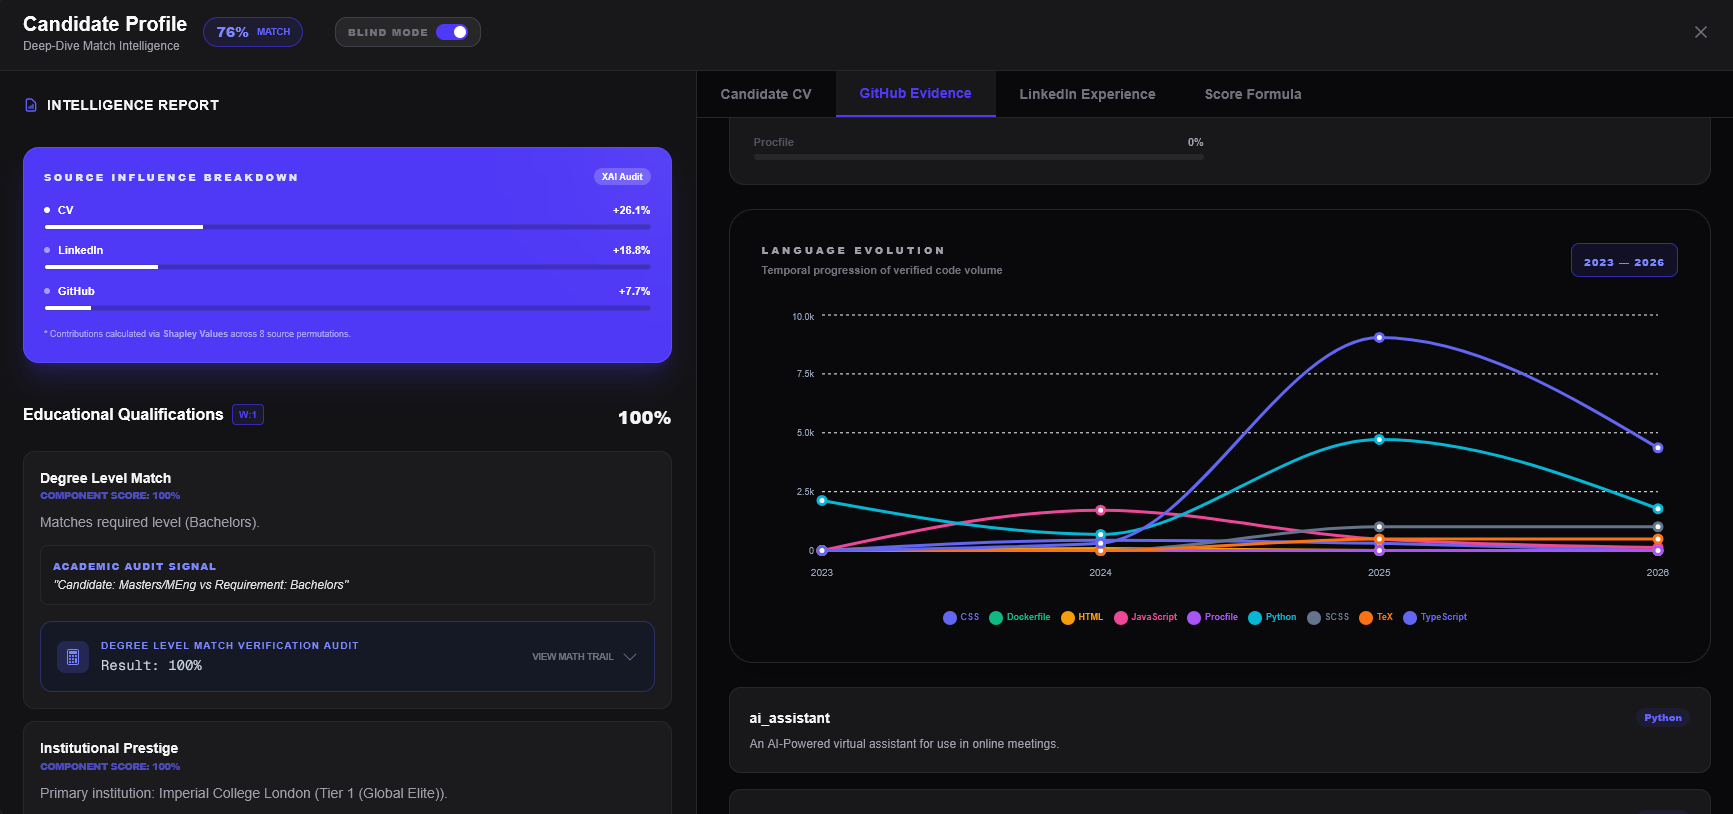
\includegraphics[width=0.95\textwidth]{implementation/screenshots/shapley_source_breakdown.png}
    \caption[Source Influence Breakdown panel]{Source influence breakdown with Shapley values per data source. In this figure,
    we show Shapley breakdown for the final match score. Shapley values for a specific metric can be viewed by clicking the ``View Math Trail''
    button}
    \label{fig:shapley_attribution}
\end{figure}


\subsection{Algorithmic Contestability}
MERIT also follows the principle of algorithmic contestability to further combat the black-box nature of these platforms.
We provide the specific evidence signals that were used to derive the score, this means that the full mathematical 
trail is provided to the recruiter to ensure that they can understand the reasoning behind the score. This in-depth
transparency is a focus of MERIT to allow recruiters to identify and override any algorithmic edge cases, or perhaps
see why a candidate got a penalisation, rather than letting this penalty go unnoticed. We ensure that the final decision
remains auditable, and aim to mitigate algorithmic bias.

The previous stage of MERIT (the execution phase) constructs both a \texttt{calculation\_summary} as well as a \texttt{results\_payload}.
For each metric, we provide the full breakdown, explicitly documenting every calculation that was performed to derive the score,
along with brief explanations for each step. Please refer to Appendix \ref{appendix:math_trail} 
for a complete step-by-step visualisation of the audit trail of an extensible metric.

This ``Glass-Box'' approach attempts to bridge the gap between complex probabilistic mathematics and practical recruitment
workflows, transforming a binary hiring decision into a defensible and interrogable process.


\subsection{Relative Cohort Normalisation}
Another common flaw with algorithmic scoring is the absence of relative context. A candidate with a year of experience may seem
weak on paper, but would be considered exceptional if the majority of the applicant pool had little to no experience. However, due
to this, the candidate would likely be undervalued if the system does not correctly highlight the difference in experience between
the candidate and the rest of the pool. To address this, MERIT also implements a dynamic cohort normalisation mechanism for the majority of
baseline metrics.

In order to achieve dynamic cohort normalisation, MERIT undergoes a two-pass approach. During the first pass of this stage, the backend
calculates the raw, absolute metrics for every candidate in the batch (such as Years of Experience, or Total GitHub repositories). Then
we aggregate these results to identify cohort maximums. In the second pass, we rerun the scoring engine, normalising candidate metrics against
the batch maximums. This approach, while not runtime efficient for extremely large datasets, ensures that MERIT's rankings remain adaptive
to the competitive landscape, rather than an arbitrary baseline.

\subsection{Glass-Box Dashboard}
\label{subsec:glass-box-dashboard}
Understandably, presenting the raw JSON \textit{results\_payload} is unreasonable due to it being inherently unscalable and poor UX.
We will briefly go over the main features of our Next.js frontend to create an intuitive, visual ``Glass-Box'' dashboard.

The first feature is probabilistic confidence labels, derived from the standard deviation $\sigma$ of the Beta distribution mentioned
in the previous chapter. We map $\sigma$ to a traffic-light badge system (Green for High, Amber for Medium, Red for Low),
allowing recruiters to instantly scan the reliability of a candidate's metric at a glance.
Non-critical penalties (e.g.\ keyword stuffing) show an amber icon on the ranking table, critical penalties (e.g.\ identity squatting) show a red warning. The significance of these labels is highlighted
more so when it comes to extensible metrics, where there is more uncertainty due to the ambiguity of how such metrics may be defined,
and calculated.

Another key innovation towards the UX of MERIT is the ``Insights'' panel. When viewing the ranking tables of a candidate, recruiters can open
a ``report'' for them, which will provide them with an overlay of, not only the candidate's score, but also how it was calculated. The metric's
calculation is also provided as a human-readable string, which can be used to understand the logic behind the score.
The panel links to the full audit trail (per-source signals, Bayesian fusion, and Shapley breakdown) and surfaces actionable 
guidance where scores are limited.
Figure~\ref{fig:glass-box-dashboards} shows the ranking table with confidence 
badges and the per-metric Insights overlay (full-size screenshots in Appendix~\ref{appendix:glass-box-ui}).

\begin{figure}[htbp]
    \centering
    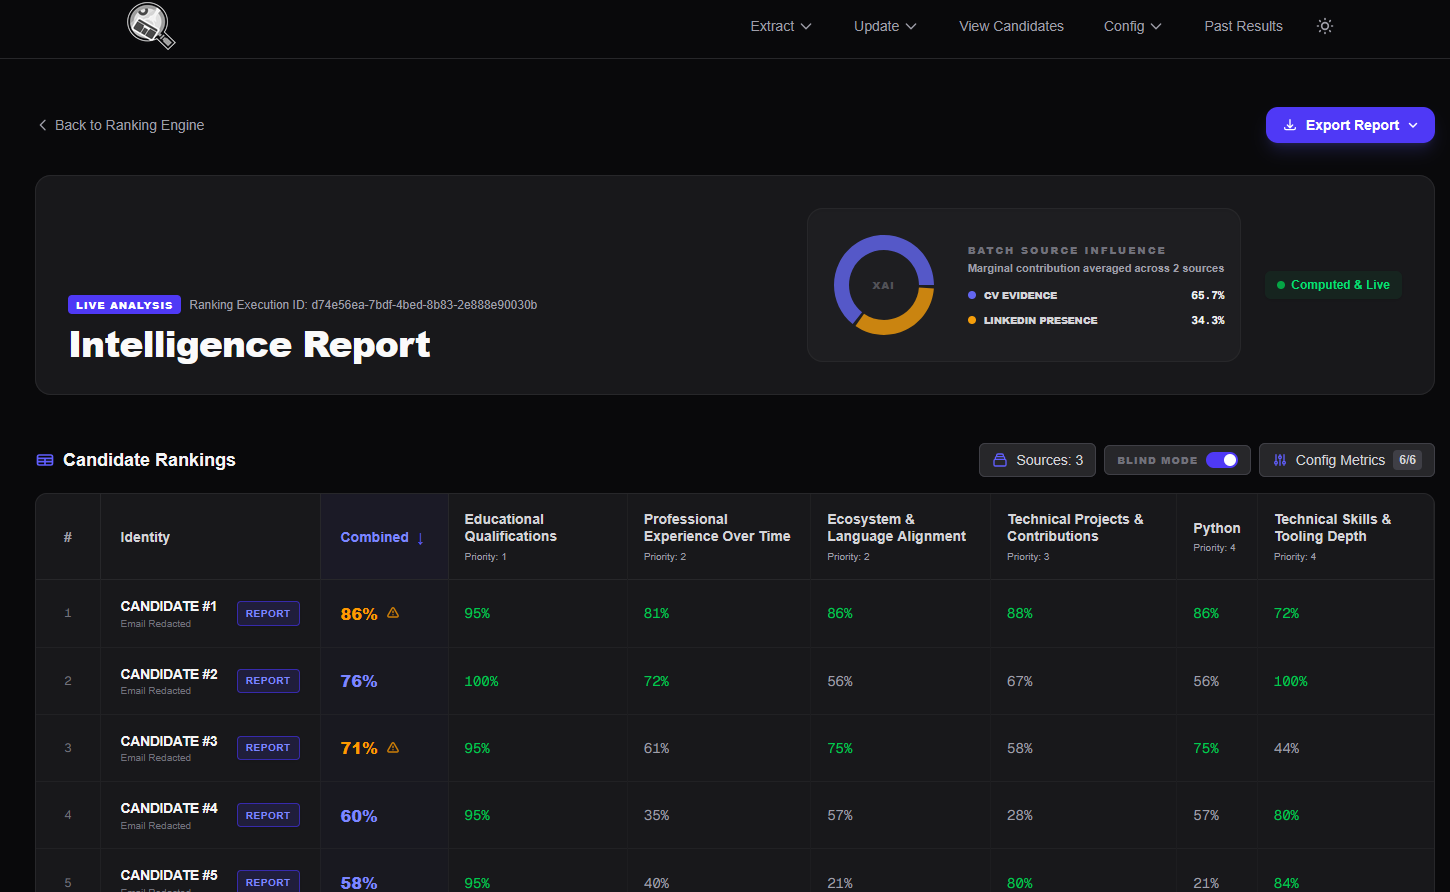
\includegraphics[height=0.17\textheight,keepaspectratio]{implementation/screenshots/candidate_rankings_dashboard.png}%
    \hfill
    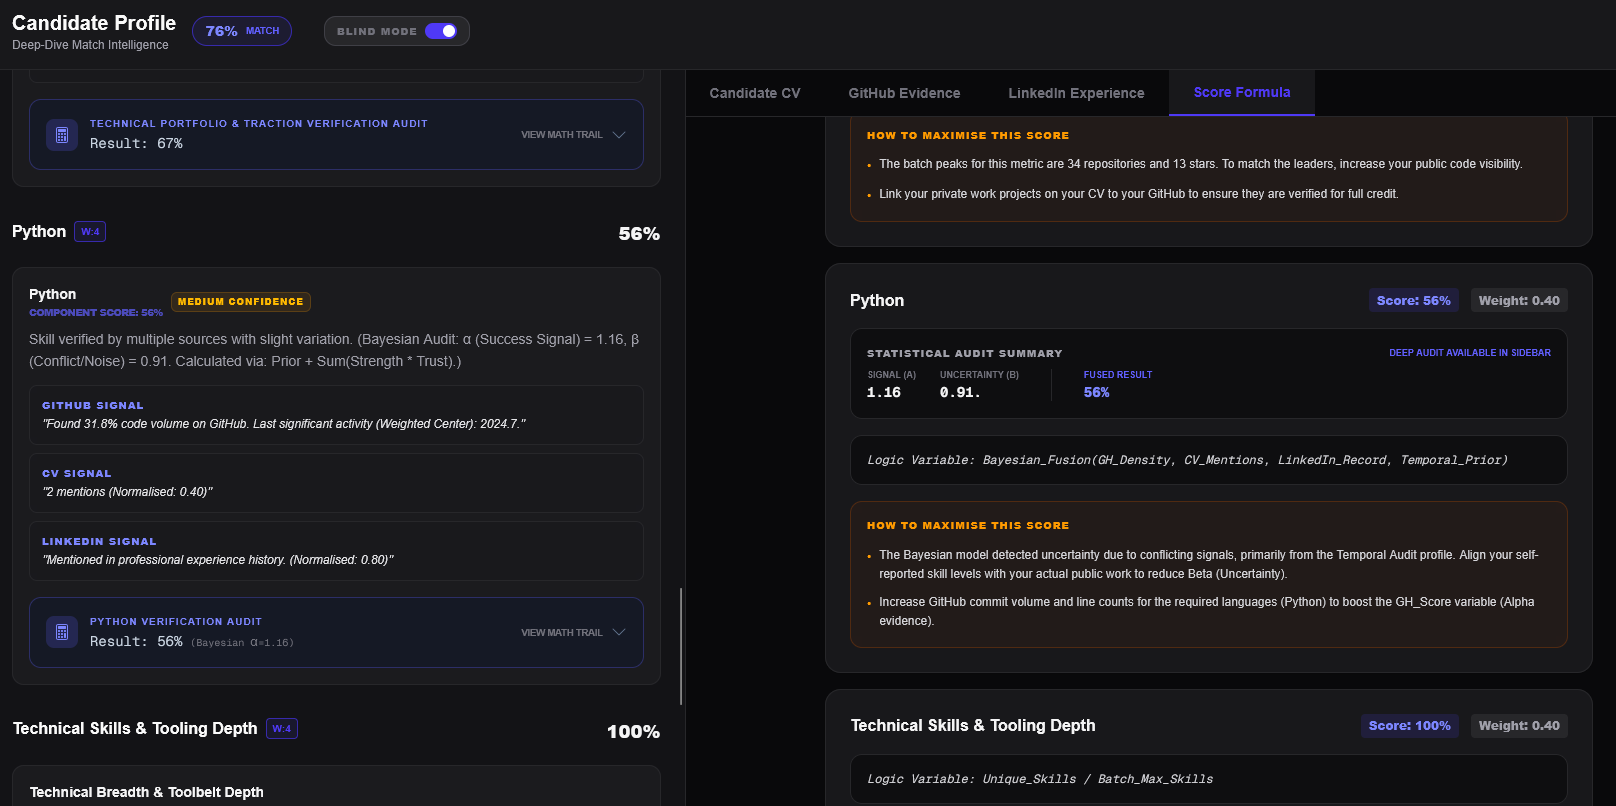
\includegraphics[height=0.17\textheight,keepaspectratio]{implementation/screenshots/metric_insights_panel.png}
    \caption[Glass-Box dashboard]{Glass-Box dashboard: Intelligence Report ranking table with confidence badges 
    (left) and Metric Insights panel for Python with audit trail (right). 
    Appendix~\ref{appendix:glass-box-ui} provides full-size versions.}
    \label{fig:glass-box-dashboards}
\end{figure}

To further aid transparency, any penalisations (such as Squatting) are also flagged to the user to highlight the negative impact of such actions on the candidate's score.
To ensure full auditability, we also provide views of each candidate's extracted data sources, so that recruiters can cross-check the audit trail.
It is also possible to view skillsets that may not have been considered by the scoring engine, for example, a configuration may have had Python
as a metric, but the candidate may have extensive work with Jupyter Notebook on their GitHub profile. If the semantic bridge mechanism fails to 
catch this, the recruiter would be able to still observe this data and potentially change their decision after accounting for this information.

\section{Bias Mitigation \& Safeguards}

TODO: Detail the cross-cutting features designed to protect the integrity of the recruitment process.

\subsection{Algorithmic Safeguards}
TODO: Implementation of the anti-keyword stuffing penalty heuristics and dynamic university tiering.

\subsection{Blind Screening Mode \& Anonymisation}
TODO: Technical implementation of redacting sensitive bias-inducing markers before UI presentation.


\chapter{Evaluation}
\label{ch:evaluation}

This chapter evaluates whether MERIT actually addresses the three gaps that were pointed out
earlier in Section~\ref{sec:relevance-to-merit}. 
Each of MERIT's pillars maps to a research question (RQ), which is derived from the literature
review earlier. Our studies are presented bottom-up (Ingestion $\rightarrow$ Fusion $\rightarrow$ 
Explainability $\rightarrow$ Human Alignment $\rightarrow$ Fairness and Scalability). Note that
this may disagree with the numerical prefixes of the studies in the repository, which follow the 
implementation order instead. Graphical representations of the studies are deferred to the appendix, 
and also cited inline.

\section{Evaluation Overview}
\label{sec:eval-overview}

\subsection{Evaluation Design and Research Questions}
\label{subsec:eval-design-rqs}

Our evaluation design is driven by the three formal research questions (RQ1--RQ3) established at the conclusion of our literature review (Section~\ref{sec:relevance-to-merit}). To briefly summarise, these questions evaluate MERIT's extensibility against rigid baselines, its multi-source fusion capabilities in the presence of conflicting candidate evidence, and the efficacy of its glass-box transparency for human decision calibration.

We map each RQ to prior work along with the associated studies and primary metrics to answer these RQs (Table~\ref{tab:eval-literature-traceability}).
We also report criteria that we use to determine the success of each RQ. Note that our success criteria are not
derived from literature, and are instead internal targets, since many results are directional due to the small sample size
in our evaluation. Both the Traditional ATS and Modern AI ATS baselines are simplified in-repository proxies
for the keyword-matching and AI-assisted ATS categories mentioned earlier in Section~\ref{sec:automated-screening}.
We do not implement a rule-based ATS baseline, the category is knockout-oriented and does not produce ranked, 
pool-wide scores comparable across candidates. Our studies instead require rankings 
(Spearman $\rho$), so we compare MERIT only against the two ranking-oriented CV-screening paradigms above. 
We do not believe this to be a significant threat to validity due to the similarities between Keyword-Matching and Rule-Based ATS systems.
For Studies~07--10, expert-consensus rankings were produced by the same four-recruiter panel described in Section~\ref{subsec:spearman-method},
who reviewed CV PDFs only,
following Lo et al.'s~\cite{lo2025aihiring} paradigm of comparing automated scores with HR judgement.
High Spearman $\rho$ measures agreement with that consensus, but cannot be generalised due to the sample size.

Our evaluation takes inspiration from software-engineering experimentation~\cite{wohlin_threats}
through construct isolation, where we use synthetic JSON personas to isolate scoring logic from 
the parsing noise of the ingestion engine.
We also take inspiration from Lo et al.'s~\cite{lo2025aihiring} evaluation paradigm, where they 
anonymise real resumes with an HR panel to evaluate the agreement between automated scores and HR judgement.
MERIT follows a related approach, where we create synthetic profiles based on real candidate data,
and then evaluate the agreement between the automated scores and HR judgement.
Threats to validity, including this design trade-off, are discussed in 
Section~\ref{sec:threats-to-validity}.


Against the internal criteria in Table~\ref{tab:eval-literature-traceability} (below), 
we do not treat every study as a pass. Study~14 meets the SUS target and Study~07 meets the directional $\rho \geq 0.7$ criterion for MERIT (Full).
However, failures are also documented: Studies~04--05 fall short of parsing $\geq 80\%$ and Spearman cohorts for Studies~08 and~10, 
fall below $\rho = 0.7$.
Outcomes by pillar are summarised in Section~\ref{sec:objectives-retrospective}.

\subsection{Evaluation Study Mapping}
\label{subsec:eval-codebase-traceability}

Each study maintains a one-to-one mapping with a prefixed subdirectory under \texttt{evaluation/} 
in the project repository~\cite{merit_repo} (e.g.\ Study~04 $\leftrightarrow$ \texttt{04-ir\_parser\_test/}).
Table~\ref{tab:eval-study-catalogue} details the purpose of each study. 
Note that Studies~02, ~03 and~06 are engineering supplements to either show proof of concept, or provide benchmarking data.

\begin{table}[H]
    \centering
    \caption[Evaluation study catalogue]{Mapping of each study to a specific research question (RQ) and purpose.}
    \label{tab:eval-study-catalogue}
    \footnotesize
    \renewcommand{\arraystretch}{1.28}
    \setlength{\tabcolsep}{5pt}
    \setlength{\extrarowheight}{1pt}
    \def\tabularxcolumn#1{m{#1}}%
    \begin{tabularx}{\textwidth}{@{}%
        >{\centering\arraybackslash}m{0.65cm}
        >{\centering\arraybackslash\hyphenpenalty=10000\exhyphenpenalty=10000}m{2.1cm}
        >{\centering\arraybackslash}X
        >{\centering\arraybackslash}m{0.48cm} @{}}
        \hline
        \textbf{No.} & \textbf{Name} & \textbf{Purpose} & \textbf{RQ} \\
        \hline
        \hyperref[subsec:study-01-comparative-ablation]{01} & Comparative ablation &
        Compare four engines on 10 personas and analyse fusion rank shifts. &
        2 \\
        \hyperref[subsec:studies-02-03-scalability]{02} & Runtime &
        Check runtime stays practical as $N$ grows (engineering supplement). &
        --- \\
        \hyperref[subsec:studies-02-03-scalability]{03} & Memory &
        Check memory stays practical as $N$ grows (engineering supplement). &
        --- \\
        \hyperref[subsec:study-04]{04} & CV parser &
        Measure CV parsing error before scoring. &
        1 \\
        \hyperref[subsec:study-05]{05} & JD parser &
        Measure JD parsing error before TF-IDF configuration. &
        1 \\
        \hyperref[subsec:study-06-adversarial]{06} & Adversarial &
        Stress-test fusion and integrity against stuffing, fraud, and gaming (RQ2 supplement). &
        --- \\
        \hyperref[subsec:study-07-spearman-high-discrimination]{07} & High disc. &
        Expert $\rho$: does MERIT Full lead when sources agree? &
        2 \\
        \hyperref[subsec:study-08-spearman-seniority]{08} & Seniority &
        Expert $\rho$: do engines over-rank seniority for an intern JD? &
        2 \\
        \hyperref[subsec:study-09-spearman-peer]{09} & Peer comp. &
        Expert $\rho$: does fusion break ties when CVs are similar? &
        2 \\
        \hyperref[subsec:study-10-spearman-dissonance]{10} & Dissonance &
        Expert $\rho$: does fusion fail when sources contradict the CV? &
        2 \\
        \hyperref[subsec:study-11-shapley-verification]{11} & Shapley &
        Check glass-box source attributions satisfy Shapley axioms. &
        3 \\
        \hyperref[subsec:study-12-bayesian-conflict-resolution]{12} & Bayes fusion &
        Check Beta--Bernoulli fusion favours demonstrated evidence over claims. &
        2 \\
        \hyperref[subsec:study-13-metric-prediction]{13} & TF-IDF &
        Check whether TF-IDF priorities match recruiter consensus. &
        1 \\
        \hyperref[subsec:hci-trial-protocol]{14} & HCI pilot &
        Check whether glass-box explanations change recruiter decisions and trust. &
        3 \\
        \hyperref[subsec:bias-mitigation-efficacy]{15} & Blind Mode &
        Check whether Blind Mode reduces proxy-driven shortlisting in the UI. &
        3 \\
        \hline
    \end{tabularx}
\end{table}

Table~\ref{tab:eval-literature-traceability} demonstrates how our literature review gaps tie directly into our evaluation studies and their success criteria. Within this mapping, temporal skill decay~\cite{arthur1998} is analysed in Section~\ref{subsec:study-08-skill-decay} as an RQ2 supporting analysis alongside the fusion studies. Additionally, Study~15 tests UI proxy debiasing~\cite{highhouse2008stubborn} rather than Shapley attributions, while Studies~02,~03, and~06 serve as engineering or adversarial supplements (Section~\ref{sec:fairness-computational-rigour}).

\begin{table}[H]
    \centering
    \caption[Literature-to-evaluation traceability]{Literature-to-evaluation traceability: mapping research questions to prior work, studies, and success criteria.}
    \label{tab:eval-literature-traceability}
    \footnotesize
    \renewcommand{\arraystretch}{1.45}
    \setlength{\tabcolsep}{6pt}
    \setlength{\extrarowheight}{2pt}
    \def\tabularxcolumn#1{m{#1}}%
    \begin{tabularx}{\textwidth}{@{}%
        >{\centering\arraybackslash}m{0.8cm}
        >{\centering\arraybackslash\hsize=1.05\hsize}X
        >{\centering\arraybackslash}m{1.9cm}
        >{\centering\arraybackslash\hsize=1.0\hsize}X
        >{\centering\arraybackslash\hsize=0.95\hsize}X @{}}
        \hline
        \textbf{RQ} & \textbf{Gap / prior work} & \textbf{Studies} & \textbf{Primary metrics} & \textbf{Success criterion} \\
        \hline
        RQ1 &
        Gugnani/Lo rigid weighting, ResumeBench parsing &
        04, 05, 13 &
        Skill $F_1$, name match, $\rho$ vs.\ recruiters &
        Parsing $\geq 80\%$, metric alignment exploratory \\
        RQ2 &
        Montandon supplementary GitHub, CV self-report bias &
        {\renewcommand{\arraystretch}{1}%
        \begin{tabular}[c]{@{}c@{}}12, 01, \\[-0.35ex] 07--10\end{tabular}} &
        Rank shift, Bayesian walkthrough, Spearman $\rho$ &
        $\rho \geq 0.7$ vs.\ experts (directional) \\
        RQ3 &
        Bogen/Raghavan transparency deficit, Lundberg Shapley &
        11, 14, 15 &
        Axiom checks, DRR, SUS, prestige gap &
        SUS $\geq 80$/100, blind gap compression \\
        \hline
    \end{tabularx}
\end{table}



\section{Evaluating Pillar 1: Extensibility}
\label{sec:foundational-ingestion-extensibility}

This section addresses \textbf{RQ1}: whether JD-driven, recruiter-configurable metrics 
and reliable ingestion can support downstream scoring.
In order for a screening system to be effective, it requires data to be ingested in a way that is accurate and reliable.
Therefore, the first area that we will evaluate is MERIT's ingestion layer, to ensure that it is reliable enough to
parse unstructured documents, specifically CVs and JDs. We do not consider structured data sources such as LinkedIn and GitHub
since there is no need to parse them, as they are already in a structured format. We begin with two studies, 
one for CVs and one for JDs, to evaluate the accuracy of the ingestion layer. Both studies compare the system's extraction 
outputs against human-verified ground-truth datasets, evaluating a total of 30 CVs (balanced across diverse layouts) and 15 JDs.
To finish the evaluation of this section, we then consider how well the metric priority predictions align with that
of a panel of recruiters, testing whether TF-IDF-derived priorities avoid the fixed-coefficient rigidity criticised in prior work 
by Gugnani and Misra~\cite{gugnani2020} and Lo et al.~\cite{lo2025aihiring}. Graphical representations for this section are 
in Appendix~\ref{appendix:ingestion-charts}.

\subsection{Evaluation Metrics}
\label{subsec:mathematical-metrics}

For our evaluation, we will be evaluating both set-based and string-based comparisons between the ground truth,
and the extracted data for our three core categories (skills, experience and identity).

\subsubsection{Skill Set Metrics}
Given $S_E$ as the set of extracted skills and $S_{GT}$ as the set of ground truth skills, we can
formulate the precision ($P_{skills}$), recall ($R_{skills}$), and F1-score ($F1_{skills}$) as follows:
{\small
\begin{align}
    P_{skills}  &= \frac{|S_E \cap S_{GT}|}{|S_E|}, &
    R_{skills}  &= \frac{|S_E \cap S_{GT}|}{|S_{GT}|}, &
    F1_{skills} &= \frac{2 P_{skills} R_{skills}}{P_{skills} + R_{skills}}
\end{align}
}

\subsubsection{Experience Recall}
For experience extraction, we mainly care about recall, since if we miss an experience, we might miss out on a
correct match. False positives are not a significant concern for this metric due to the strict nature of experience
extraction.

Given a set of ground truth experiences $E_{GT}$, and a set of extracted experiences $E_E$, we define a
successful match as follows:
\begin{equation}
    \text{Match}(e_{gt}) = \mathbb{I}\left(\exists e_e \in E_E \text{ s.t. } \text{norm}(e_{gt}) \subseteq \text{norm}(e_e)\right)
\end{equation}

Experience Recall ($R_{exp}$) is thus:
\begin{equation}
    R_{exp} = \frac{1}{|E_{GT}|} \sum_{e_{gt} \in E_{GT}} \text{Match}(e_{gt})
\end{equation}

\subsubsection{Identity and Metadata Matching}
When it comes to the extraction of identity for both CVs and JDs, we only consider the exact matches, since
metrics such as precision and recall are not applicable in that case. For CVs we do this for both name and 
email addresses. For the JD, while we do perform a similar operation, we are less strict with the matching,
it is considered a match if the ground truth label is a substring of the extracted label to account for the 
difficulty of matching the company name exactly in JDs.

\subsection{Study 04: CV Ingestion Accuracy}
\label{subsec:study-04}

We first evaluate the accuracy of the CV parser, extracting candidate data from 15 single-column CVs. We also
replicate this data across 15 multi-column CVs, ensuring that the content is the same for a given candidate,
to also evaluate the impact of a CV's layout on the accuracy of the parser. The CVs are designed to be diverse
in nature, across different roles and seniority levels. We craft a ground truth dataset for each candidate,
with the author verifying the accuracy and completeness of these JSON payloads.
Table~\ref{tab:cv_parser_results} presents the compiled results.

\begin{table}[htbp]
    \centering
    \caption[Study~04: CV ingestion by layout]{Study~04: CV ingestion accuracy by layout ($N=30$).}
    \label{tab:cv_parser_results}
    \merittablesize
    \setlength{\tabcolsep}{6pt}
    \begin{tabular}{l|c|c|c}
        \hline
        \textbf{Metric} & \textbf{Single-col.\ ($N{=}15$)} & \textbf{Multi-col.\ ($N{=}15$)} & \textbf{Overall ($N{=}30$)} \\
        \hline
        Skill Extraction Precision   & 69.6\%  & 69.6\%  & 69.6\%  \\
        Skill Extraction Recall      & 38.6\%  & 38.6\%  & 38.6\%  \\
        Skill Extraction $F_1$-Score & 49.4\%  & 49.4\%  & 49.4\%  \\
        Experience Recall            & 34.3\%  & 44.7\%  & 39.5\%  \\
        Name Match Rate              & 53.3\%  & 13.3\%  & 33.3\%  \\
        Email Match Rate             & 100.0\% & 100.0\% & 100.0\% \\
        \hline
    \end{tabular}
\end{table}

The distribution of individual scores across the template pool is plotted in
Figure~\ref{fig:ingestion-combined} (panel~a, Appendix~\ref{appendix:ingestion-charts}).

\subsubsection{Qualitative Analysis}

We have four key findings from this study, each with different root causes.

The first finding is that skill extraction is not hindered by the layout of a CV, but rather the dictionary that it is 
using to identify the skills. We can observe this as both layouts achieve the same precision, recall and F1-score ($69.6\%$, $38.6\%$ and $49.4\%$ respectively).
The source that we collect skills from, Devicon, catalogues programming languages as well as frameworks, however, it completely
ignores categories that are common on real engineering CVs. One such example is tooling for observability, such as Prometheus and Grafana.
The precision indicates that what is found is correct for the most part, but the limiting issue is the dictionary we use, rather than the 
logic of our extraction process. This finding is consistent with resume-parsing benchmarks such as ResumeBench \cite{emnlp2025resumebench}.

Another important observation is that the detection of candidate name drops sharply under multi-column layouts.
There is a 40\% drop between single-column and multi-column layouts when it comes to identifying the candidate name.
In a typical single-column layout, candidate name is generally the first item in the CV, at the top of the document.
However, for multi-column layouts, this is often not the case. This is a clear example of structural failure in the 
ingestion layer due to our parser having simplistic heuristics for name extraction.

We also find that email extraction is fully robust, achieving a 100\% match rate across both layout types,
confirming that our regex-based extraction process is not hindered by the layout of the candidate CV.

Finally, we end with counterintuitive results for experience extraction, noting that experience recall rises from
34.3\% in single-column layouts to 44.7\% in multi-column layouts. The structural difference between the two layouts
is definitely the reason, however, initially it was not clear why it was higher in the multi-column layout. Further
inspection leads us to believe that the reason is due to Single-Column layouts presenting experience as inline, with
multiple pieces of information on the same line, separated by a pipe character, or other delimiters. This must
be parsed as a single unit before we can isolate details such as the employer name and the role. Multi-column
layouts tend to have less width due to the introduction of more columns, so candidates tend to have these details on
separate lines. This actually makes it easier for the parser to isolate details, which could suggest why multi-column
layouts have better recall for experience compared to single-column layouts.

CVs are unstructured documents, and as such, there is a need for structured, schema-based data sources to be able
to account for parsing errors that may arise from CV ingestion (such as a LinkedIn profile). In real-world
applications, it is likely that commercial Applicant Tracking Systems (ATS) suffer from the same structural
parsing failures that we have observed in our study. The black-box nature of these screening systems would 
make it difficult for recruiters to know if this is actually the case for why a candidate receives a low score.
It is for this reason that candidates are strongly advised to use simple, single-column templates, as discussed in practitioner ATS guidance \cite{marr2019}.
Recruitment-management systems also tend to discard applicants who fail to mirror job-description keywords and criteria \cite{fuller2021hiddenworkers}.
In turn this uncovers a systemic bias: automated screening systems penalise highly qualified candidates if the
layout of their CV confuses the parser, consistent with the parsing failures we observed.

\textbf{Outcome:} Does not meet the internal parsing $\geq 80\%$ target (skill $F_1 = 49.4\%$, name match = $33.3\%$).
Precision is acceptable, but dictionary recall and multi-column name heuristics bound RQ1 ingestion.

\subsection{Study 05: Job Description Accuracy}
\label{subsec:study-05}
The JD parser was evaluated in a similar manner, with a total of 15 job descriptions across different software
engineering roles to ensure a wide range of formats and technical requirements. The compiled mean results
are summarised in Table~\ref{tab:jd_parser_results}, the per-document distribution is in
Figure~\ref{fig:ingestion-combined} (panel~b, Appendix~\ref{appendix:ingestion-charts}).

\begin{table}[htbp]
    \centering
    \caption[Study~05: JD extraction accuracy]{Study~05: mean JD extraction accuracy ($N=15$).}
    \label{tab:jd_parser_results}
    \merittablesize
    \setlength{\tabcolsep}{6pt}
    \begin{tabular}{l|l|r}
        \hline
        \textbf{Metric} & \textbf{Evaluation focus} & \textbf{Mean (\%)} \\
        \hline
        Skill Requirements Precision   & Target skill relevance       & 60.02\% \\
        Skill Requirements Recall      & Target skill coverage        & 34.13\% \\
        Skill Requirements $F_1$-Score & Overall requirement fidelity & 40.81\% \\
        Job Title Match Rate           & Role identification        & 46.67\% \\
        Company Match Rate             & Employer identification    & 6.67\%  \\
        \hline
    \end{tabular}
\end{table}

\subsubsection{Qualitative Analysis \& Strategic Ingestion Failure Cases}

Unlike CVs, which serve as concise professional summaries, Job Descriptions (JDs) are inherently
marketing-oriented documents designed to attract candidates. As a result, they are often dense with corporate
boilerplate, such as institutional missions, values, wellness benefits, and equal opportunity clauses.
This structural noise significantly degrades parsing accuracy. Because section headings are frequently
styled with generic tags (e.g.\ ``About Us'' or ``Who We Are''), the parser struggles to isolate core technical
qualifications from general corporate copy. This lexical contamination is directly reflected in the metrics,
driving a low Skill Recall of 34.13\% and restricting Skill Precision to 60.02\%, as the extraction engine
fails to separate critical technology requirements from marketing jargon.

The most notable observation within this evaluation is the poor performance of company name extraction, with a match rate
of 6.67\%, only successfully extracting one of the fifteen JD company names. The reason for this is structural, rather than 
semantics. Employers often represent company names in text that is not easily extractable by a parser, for example, they
represent their name as a logo or image. Text extractors (in our case, pdfminer) cannot extract this textual information from
an image, it is therefore forced to rely on the ``About Us'' section. If the name is not present in this section, or 
referred to via generic pronouns (such as ``Our company''). Then the extraction process fails. Fortunately, this is a non-critical
bottleneck, since the only usage of this metric is for the recruiter to know the company name, and not for the scoring process.
It is a convenience feature rather than a core functional requirement.

\textbf{Outcome:} Does not meet parsing $\geq 80\%$ (skill $F_1 = 40.81\%$).
While employer extraction is not critical for ranking, the JD skill recall still fails to meet RQ1's success criteria.

\subsection{Study 13: Metric Prediction vs Recruiter Alignment}
\label{subsec:study-13-metric-prediction}

While the past two studies evaluate MERIT's extraction, this study instead evaluates the weighting side of RQ1. We
aim to test whether TF-IDF derived metric priorities are able to align with expert consensus, as opposed to merely
having a fixed coefficient scheme.
We test \textbf{H1} (positive Spearman $\rho$ within each role) and \textbf{H2} (low MAE versus consensus on MERIT's 1--5 scale,
where 1 = essential and 5 = optional).

\subsubsection{Method}
When generating the market corpus, we employ Tonic.ai to synthesise a dataset of 100 JDs, providing a relatively realistic
dataset to aid in this evaluation. We have three hold-outs which are excluded from the generation of the corpus, that being a Junior 
Frontend, senior ML and Lead DevOps role. This is to prevent TF-IDF from being biased towards these roles. We have one global corpus,
we do not partition by seniority nor by role family.

On the testing side, we have two recruiters and two academic peers who are tasked with weighting the metrics given a JD. We intentionally
hide the suggestions that TF-IDF would have suggested to ensure fairness. Our consensus is determined by the median of these ratings, and 
we compare these results to TF-IDF suggestions, calculating the exact match, mean absolute error (MAE) and Spearman $\rho$.
The graphical representations for this study are available in Appendix~\ref{appendix:metric-prediction-charts}.

\subsubsection{Results}
As shown in Table~\ref{tab:study-13-metric-alignment}, TF-IDF is not well
calibrated for exact matches. We can see that none of the roles manage $\geq 50\%$ for the exact match rate between 
TF-IDF and recruiter consensus. However, we can observe that in most cases, Spearman $\rho$ is positive, showing some
alignment between the TF-IDF predictions and the recruiter consensus. This is a good sign, as it 
indicates that the TF-IDF predictions are generally in the right direction, but not necessarily a perfect match.
\begin{table}[htbp]
    \centering
    \caption[Study~13: TF-IDF vs consensus]{Study~13: TF-IDF vs.\ consensus ($N=4$, $n=27$ skill--role pairs).}
    \label{tab:study-13-metric-alignment}
    \merittablesize
    \setlength{\tabcolsep}{6pt}
    \begin{tabular}{l|c|c|c|c}
        \hline
        \textbf{Hold-out role} & \textbf{Skills} & \textbf{Exact match} & \textbf{MAE} & \textbf{Spearman $\rho$} \\
        \hline
        Junior Frontend (React) & 9  & 44.4\% & 0.78 & 0.52 \\
        Senior ML Engineer       & 8  & 25.0\% & 1.88 & $-0.45$ \\
        Lead DevOps / Platform   & 10 & 20.0\% & 1.20 & 0.40 \\
        \hline
        \textbf{Aggregate} ($n{=}27$) & 27 & 29.6\% & 1.26 & 0.25 \\
        \hline
    \end{tabular}
\end{table}

Of the 27 skill--role pairs, eight achieve exact agreement and a further nine differ by only one Likert band (63\% within $\pm 1$).
The near misses show that our metric predictions should be treated as reasonable guidance, rather than simply a default value.


\subsubsection{Limitations and their Implications}
\label{subsubsec:study-13-limitations}

This is a pilot study ($N = 4$ evaluators, $n = 27$ pairs), and the results are not generalisable to the wider market.
We are not able to conduct a larger panel study due to the time and resource constraints of this project.

Another limitation is due to the way we create the corpus, or rather, the fact that we only use one corpus for all TF-IDF calculations.
Due to this, we encounter cross-role IDF interference. To take an example, let's consider Python, a language used in many different roles such
as backend development, machine learning, data science and more. Since Python is common in these roles, it will inevitably be in a significant
proportion of job descriptions and, as a result, we would have a high IDF score, regardless of the role, making it seem like Python is 
always a common skill. This down-ranks Python on the metric predictions, regardless of the role.

In this study, we also did not ask our participants to spread their ratings evenly between the 1 and 5 scale. Compare this to TF-IDF
which has an in-built min--max normalisation to the range $[1.0, 5.0]$ which ensures a relatively even distribution of these ratings.
This disparity in rating distribution is likely to play a role in our evaluation results, particularly the exact match rate. 
That mismatch can depress exact-match rate and $\rho$ without invalidating the pilot, it is a
comparison caveat we report alongside the within-$\pm 1$ band counts above. Cross-study validity threats are summarised in
Section~\ref{sec:threats-to-validity}.

\textbf{Outcome:} Exploratory RQ1 criterion only: aggregate Spearman $\rho = 0.25$ with mixed hold-outs 
(Table~\ref{tab:study-13-metric-alignment}).
\textbf{H1} is partly supported and \textbf{H2} is not met. TF-IDF priorities should be treated as guidance, 
not automatic weights, with recruiter overrides on the frontend.

\subsection{Downstream Mitigation}
\label{subsec:downstream-mitigation}

These quantitative findings empirically justify two of MERIT's three core architectural pillars.

\subsubsection{Multi-Source Fusion (Pillar 2)}

The recall of 38.6\% means that CV-only screening will often miss the majority of a candidate's technical competencies
under the Devicon dictionary. The drawbacks of a dictionary-based approach are clearly visible here, as well as the 
reliance on a single source of truth for areas such as skill extraction. By ingesting other sources into candidate
scoring (such as GitHub repository language statistics and LinkedIn skill endorsements), MERIT can recover 
skills that the CV parser may have failed to recognise. 


\subsubsection{Glass-Box Explainability (Pillar 3)}
The issues presented above would often fail to be surfaced to recruiters in typical black-box scoring systems.
This highlights the need for a system that can surface these parsing failures to recruiters. The addition of 
MERIT's explainability layer achieves this by providing in-depth reviews of both the candidate's original 
data, as well as what MERIT was able to extract from it. This ensures that recruiters are able to audit and alter
their decisions based on the information that MERIT was able to gather. For example, a recruiter may observe that
a metric, such as Python, may not have been extracted from the candidate CV due to a parser error. The recruiter would
then be able to either observe the original CV to challenge the claim, or perhaps consider other data sources.
\section{Evaluating Pillar 2: Multi-Source Fusion}
\label{sec:evaluating-multi-source-fusion}

% Helper macros for evaluation tables (defined at top to prevent duplicate definition/undefined command errors)
\newcommand{\splithead}[2]{\begin{tabular}[c]{@{}c@{}}\textbf{#1} \\ \textbf{#2}\end{tabular}}
\newcommand{\splitcand}[2]{\begin{tabular}[c]{@{}l@{}}#1 \\ #2\end{tabular}}
\newcommand{\splitdesc}[2]{\begin{tabular}[c]{@{}l@{}}#1 \\ #2\end{tabular}}
\newcommand{\splitcell}[2]{\begin{tabular}[c]{@{}c@{}}\##1 \\ (#2)\end{tabular}}
\newcommand{\rankonly}[1]{\##1}

This section evaluates MERIT's multi-source fusion model, directly addressing RQ2. To ensure a thorough
evaluation, we proceed from the bottom up. We first demonstrate how skill decay can affect a candidate's score, 
from there, we then test the Bayesian Fusion process, evaluating the effects of conflict resolution and 
testing to see whether MERIT rewards demonstrated evidence over claimed evidence. From there, we conduct
an algorithmic study against baseline ATS scoring engines to compare alignment to expert decisions.

For studies involving ATS scoring engines, we specifically refer to four scoring engines. We have a \textbf{Traditional ATS}
baseline that replicated the keyword-matching system mentioned in Section~\ref{sec:automated-screening}. We also include a 
\textbf{Modern AI ATS} baseline that replicated the AI-assisted system mentioned in that section. For the evaluation
we also separate MERIT into two engines, one that only considers CV data, and one that considers all implemented
data sources (CV, GitHub, LinkedIn) to isolate the impact of the multi-source fusion layer.

The baselines are not commercial products, they are in-repository baselines that proxy keyword-matching and AI-assisted 
ATS systems. We intentionally omit rule-based engines as they are knockout-oriented, they do not rank candidates. 

We isolate the scoring logic by assuming perfect data extraction, using synthetic candidate JSON profiles. 
This removes parsing noise, establishing a clean mathematical baseline to accurately evaluate scoring logic, 
temporal decay, and conflict resolution. The validity implications for this are detailed
in Section~\ref{subsec:internal-validity}.

\subsection{Skill-Decay Sensitivity Analysis (RQ2 Supplement)}
\label{subsec:study-08-skill-decay}

Prior research on skill retention shows that unused workplace skills deteriorate over time~\cite{arthur1998}. 
The purpose of this study is to test whether our modelled skill decay provides a large enough mathematical 
separation between a candidate's active and stale skills to rank them appropriately. 

While this analysis does not strictly calibrate the decay constant ($\lambda$) against Arthur et al.'s empirical 
effect sizes, it models retention using the exponential decay curve defined in Equation~\ref{eq:exponential_decay}. 
Here, $S_0$ is the initial unweighted skill score and $\lambda$ is the decay constant. 

In MERIT, we set $\lambda \approx 0.25$ (yielding a half-life of $t_{1/2} \approx 2.77$ years, see 
Section~\ref{subsec:skill-decay-modelling}). To illustrate this 
sensitivity: for two otherwise identical profiles (active vs.\ stale), a 6-year stale signal yields 
$S(6) = S_0 e^{-0.25 \cdot 6} \approx 0.223 S_0$. Because the stale signal retains only 22.3\% of its active 
value, it creates a clear ranking separation. Consequently, the outcomes of this study should be seen as 
directional rather than strictly quantitative.

\subsection{Study 12: Bayesian Conflict Resolution}
\label{subsec:study-12-bayesian-conflict-resolution}

The reasoning for MERIT's multi-source fusion layer is to be able to reward candidates who are able to demonstrate their skills 
with publicly available evidence. This is particularly important for extensible metrics, where said metric is tied directly
to the job description that it was derived from. We believe it to be essential to reward candidates who can prove that they are
fit for the role, rather than just claim to be fit for it. In this study, we verify the Beta-Bernoulli conjugate updating 
implementation \cite{gelman2013bayesian} by contrasting a claims-only candidate against a demonstration-only candidate on the same extensible 
metric, motivated by the need to down-weight self-reported CV claims that personnel research shows are frequently 
embellished~\cite{henle2019_resume_fraud,dunning2004}. We also evaluate full-evidence and zero-evidence bounds to establish the 
mathematical ceiling and floor of the scoring engine.

In this walkthrough, the maximum signal that claims-only sources can achieve is $0.8$, while the maximum signal for demonstration-only signals
is uncapped at $1.0$. We start from priors $\alpha_0 = \beta_0 = 0.1$, and the step-by-step walkthrough for these two core profiles is given in Table~\ref{tab:bayesian-walkthrough}.

\begin{table}[htbp]
    \centering
    \caption[Study~12: Claims vs.\ demonstration walkthrough]{Study~12: Step-by-step fusion for the two core profiles.}
    \label{tab:bayesian-walkthrough}
    \small
    \setlength{\tabcolsep}{5pt}
    \begin{tabular}{l c c c c c c}
        \toprule
        \textbf{Step} ($i$) & $s_i$ & $c_i$ & $\alpha$ & $\beta$ & \textbf{Score} & $\sigma$ \\ \midrule
        \multicolumn{7}{c}{\textbf{Claimed only, no demonstration}} \\ \midrule
        0. Prior            & ---   & ---   & 0.100 & 0.100 & 0.500 & 0.456 \\
        1. CV               & 0.800 & 0.500 & 0.505 & 0.205 & 0.711 & 0.347 \\
        2. GitHub           & 0.000 & 0.900 & 0.506 & 1.106 & 0.314 & 0.287 \\
        3. LinkedIn         & 0.800 & 0.200 & 0.674 & 1.154 & 0.369 & 0.287 \\ \midrule
        \multicolumn{7}{c}{\textbf{Demonstrated only, no claims}} \\ \midrule
        0. Prior            & ---   & ---   & 0.100 & 0.100 & 0.500 & 0.456 \\
        1. CV               & 0.000 & 0.500 & 0.105 & 0.605 & 0.148 & 0.271 \\
        2. GitHub           & 1.000 & 0.900 & 1.006 & 0.606 & 0.624 & 0.300 \\
        3. LinkedIn         & 0.000 & 0.200 & 1.014 & 0.814 & 0.555 & 0.296 \\ \bottomrule
    \end{tabular}
\end{table}

Step-by-step parameter commentary for these core scenarios is in Appendix~\ref{appendix:bayesian-fusion-walkthrough}.
Table~\ref{tab:bayesian-scenario-comparison} subsequently summarises the final scores of these profiles alongside the empirical ceiling and floor bounds.
Figure~\ref{fig:bayesian-fusion-convergence} (Appendix~\ref{appendix:bayesian-fusion-charts}) plots the step-by-step trajectories of the two core scenarios.

\begin{table}[htbp]
    \centering
    \caption[Study~12: Claims vs.\ demonstration]{Study~12: Hypothetical claims vs.\ demonstration profiles, bounded by full and zero evidence.}
    \label{tab:bayesian-scenario-comparison}
    \small
    \setlength{\tabcolsep}{4pt}
    \begin{tabular}{l c c c c c}
        \toprule
        \textbf{Scenario} & $s_{\mathrm{CV}}$ & $s_{\mathrm{GH}}$ & $s_{\mathrm{LI}}$ &
        \textbf{Final} & $\sigma$ \\ \midrule
        Full evidence (Max claims and demonstration) & 0.8 & 1.0 & 0.8 & 0.861 & 0.206 \\
        Demonstrated only, no claims   & 0.0 & 1.0 & 0.0 & 0.555 & 0.296 \\
        Claimed only, no demonstration & 0.8 & 0.0 & 0.8 & 0.369 & 0.287 \\
        Zero evidence (No claims, no demonstration) & 0.0 & 0.0 & 0.0 & 0.062 & 0.144 \\ \bottomrule
    \end{tabular}
\end{table}

\textbf{The divergence point.} At the GitHub step (Table~\ref{tab:bayesian-walkthrough}, row~2, 
Figure~\ref{fig:bayesian-fusion-convergence}), the two core profiles diverge sharply. The 
demonstration-only candidate reaches $0.624$, while the claims-only candidate falls to $0.314$, a gap of 31 percentage points. This 
reflects the higher source confidence assigned to demonstrated GitHub evidence ($c_{\mathrm{GH}} = 0.9$), and the fact that a zero 
GitHub signal actively contradicts the CV claim rather than leaving it unchallenged.

\textbf{The claims-only penalty.} For the claims-only profile, a capped CV assertion ($s_1 = 0.8$, $c_1 = 0.5$) initially lifts the score from $0.500$ to $0.711$. This is
broadly the sort of outcome a CV-only screening pipeline might produce. If the candidate had simply not linked a GitHub profile (a missing source), 
the fusion engine would stop here and their score would remain at $0.711$, successfully avoiding unfair penalisation for lacking an open-source presence. 
However, because they linked a GitHub profile that contained no evidence for this specific metric, the zero signal actively contradicts the CV's claim. After GitHub contradicts the claim, the score crashes to $0.314$, and a
further LinkedIn endorsement ($s_3 = 0.8$, $c_3 = 0.2$) only recovers it to $0.369$. Additional self-report cannot substitute for missing
public work samples.

\textbf{The demonstration reward.} The demonstration-only profile follows the reverse pattern. An empty CV ($s_{\mathrm{CV}} = 0$) briefly pulls the score down to $0.148$
before GitHub ingestion, after which strong demonstrated evidence lifts it to $0.624$ and the final fused score settles at $0.555$. MERIT
rewards demonstrated evidence over claimed evidence, and this is an intentional design choice. Self-reported CVs are prone to embellishment,
while demonstrated evidence is harder to game, and requires a candidate to actually use the skill in their own projects or daily work.
The system favours candidates who can back up their skills with public work, while recording uncertainty when there is a lack of evidence.

\textbf{Deterring strategic omission.} One might ask whether a candidate could ``game'' the system by intentionally withholding a 
data source (like GitHub) to avoid the risk of a low signal contradicting their CV. However, because MERIT caps the strength and 
lowers the confidence of self-reported sources, a candidate who omits demonstrated evidence artificially ceilings their maximum 
possible score for that metric (and potentially all others). While their score will not actively crash, they leave the door wide 
open for other candidates with verified public work to easily surpass them in the final rankings. This inherently deters the strategic omission of data sources.

\subsection{Study 01: Comparative Engine and Source Ablation}
\label{subsec:study-01-comparative-ablation}

To evaluate the benefits and drawbacks of MERIT's multi-source fusion model, we compare it against three other baseline screening engines on
ten synthetic personas (\texttt{evaluation/01-comparative\_study/}).
The first is \textbf{Traditional ATS}, an in-repository engine that replicates the keyword-matching ATS category in
Section~\ref{sec:automated-screening}.
It scores candidates solely on the count of matching keywords in their CV.
The second is \textbf{Modern AI ATS}, an in-repository engine that replicates the AI-assisted ATS category.
It computes cosine similarities between CV embeddings and Job Description (JD) embeddings using Sentence-BERT (SBERT)~\cite{reimers2019sentence}.
To reiterate, neither baseline is a commercial ATS platform.
We also run \textbf{MERIT (CV Only)} which only considers CV data, and \textbf{MERIT (Full)} which considers all implemented data sources.

We can observe the rankings of the engines in Table~\ref{tab:algorithmic-ablation}, where rank~1 is considered the best
candidate--job fit and rank~10 the worst. The fusion shift column records how each candidate's rank changes from MERIT (CV Only) to MERIT (Full).
See Figure~\ref{fig:rank-displacement-bump-chart} (Appendix~\ref{appendix:rank_displacement}) for a bump-chart visualisation.


\begin{table}[H]
    \centering
    \caption[Study~01: Comparative benchmark rankings]{Study~01: ordinal ranks across four screening engines ($N=10$ personas, rank~1 = best fit).
    Fusion shift is the rank change from MERIT (CV Only) to MERIT (Full).}
    \label{tab:algorithmic-ablation}
    \vspace{1.5ex}
    \small
    \setlength{\tabcolsep}{5pt}
    \begin{tabular}{l l c c c c c}
        \toprule
        \textbf{Candidate} & \textbf{Profile} & \textbf{Trad.} & \textbf{Mod. AI} & \textbf{CV} & \textbf{Full} & \textbf{Fusion shift} \\ \midrule
        Alex Rivers        & Verified elite    & \rankonly{5}  & \rankonly{1}  & \rankonly{1}  & \rankonly{1}  & 0 \\
        Felix Vance        & Identity~mismatch & \rankonly{3}  & \rankonly{6}  & \rankonly{2}  & \rankonly{3}  & $-$1 \\
        Jordan Smith       & Hidden gem        & \rankonly{10} & \rankonly{9}  & \rankonly{10} & \rankonly{2}  & \textbf{+8} \\
        Buzz Ward          & Keyword~stuffer   & \rankonly{2}  & \rankonly{5}  & \rankonly{3}  & \rankonly{6}  & $-$3 \\
        Ghost Gary         & Unverified        & \rankonly{4}  & \rankonly{7}  & \rankonly{5}  & \rankonly{8}  & $-$3 \\
        Sam Old            & Stale profile     & \rankonly{6}  & \rankonly{8}  & \rankonly{7}  & \rankonly{5}  & +2 \\
        Vince Vault        & High-tenure Fraud & \rankonly{1}  & \rankonly{4}  & \rankonly{4}  & \rankonly{9}  & \textbf{$-$5} \\
        Fiona Frost        & Skill absence     & \rankonly{8}  & \rankonly{3}  & \rankonly{6}  & \rankonly{7}  & $-$1 \\
        Kim Junior         & Entry-level       & \rankonly{9}  & \rankonly{10} & \rankonly{9}  & \rankonly{4}  & +5 \\
        Carl Corp          & Closed-source     & \rankonly{7}  & \rankonly{2}  & \rankonly{8}  & \rankonly{10} & $-$2 \\ \bottomrule
    \end{tabular}
\end{table}

In the table, we can observe how the Traditional ATS prioritises keyword density and tenure (Vince Vault \#1 and Buzz Ward \#2),
while the Modern AI ATS prioritises CV semantics behind the keywords, rather than blindly prioritising density (Alex Rivers \#1 and Buzz Ward \#5).
Similar behaviour can be observed for CV-only MERIT, but note the lack of focus on tenure, specifically Carl Corp (\#2 $\rightarrow$ \#8 from Modern AI ATS to CV-only MERIT).
For MERIT (Full), we can observe that the multi-source data for Jordan Smith and Kim Junior are recognised, leading to rank shifts of +8 and +5 respectively.

\textbf{Jordan Smith: hidden gem.} The key finding from this study is from the hidden gem persona, Jordan Smith. The candidate is a low-tenure developer, only having
a year of formal experience on his CV, but has a strong GitHub presence that he has not mentioned well on his CV. While this is not a common scenario,
we mainly highlight this to show the cases where a candidate may not present themselves in an ATS-friendly manner, leading to them being overlooked by these engines.

MERIT (Full)'s integration of multi-source data allows the engine to take his extensive GitHub data into account, noting his public work in both Java and TypeScript,
two highly weighted skills in the JD. Due to the candidate having a significant amount of evidence compared to his peers, he is able to rise from rank \#10 to rank \#2.
This candidate is a clear example of how MERIT can reveal candidates who may be overlooked by current state-of-the-art single-source ATS engines that often
fall into the ``Resume Black Hole''~\cite{fuller2021hiddenworkers}.

\textbf{Carl Corp: proprietary data gap.} MERIT is a system that thrives on the presence of public data, candidates are encouraged to showcase their best work on their public profiles.
Carl Corp is a candidate who presents a trade-off that MERIT must face, that being candidates who are not able to publicly showcase their work.
Due to the candidate's commits being in private repositories, we are unable to determine his true skill set, leading to him being down-weighted by the engine,
since he is not able to benefit from the multi-source fusion layer to its full potential. Under MERIT (Full), he falls from rank \#2 to rank \#10.

Here, we present a ``Proprietary Data Gap'' scenario, showing that MERIT is more likely to favour a junior with public work, over an experienced candidate
with private data. MERIT trades off verifiable evidence for the accessibility of such evidence.

\textbf{Vince Vault: identity squatting.}\label{subsubsec:identity-mismatch-resolution} Due to the difficulty of gaming demonstrated evidence, MERIT prepares for the possibility of candidates who may
attempt to pass off another's work as their own. We refer to this act as ``identity squatting''.
In our study, we present Vince Vault as a candidate who performs this malicious action. Vince is a candidate who claims
ten years of experience and also an expert in Java, but it is likely that he is unable to show this evidence through his own public work.
Because of this, the candidate, in this scenario, submits a link to another candidate's GitHub account so that someone else's demonstrated work can support
his application. Traditional ATS and Modern AI ATS do not consider multi-source data, only relying on his CV claims, as such, 
he is able to rank highly on both engines by simply claiming to have the skills. The same observation can be made for MERIT (CV Only), 
where he is able to rank highly on CV text alone.

Once we account for multi-source data, MERIT (Full) detects a name difference between the candidate's CV and GitHub account, specifically, the GitHub
account belongs to another individual, ``Alice Smith''. The Integrity Engine penalises this mismatch, leading to Vince Vault falling from rank \#4 to rank \#9
between MERIT (CV Only) and MERIT (Full). To ensure fairness, we surface this information to the recruiter, providing the full names associated with the data sources
to the user to investigate further.

Identity squatting is rare in practice, but it is an important edge case to consider to ensure the integrity of the system.
\section{Evaluating Pillar 3: Glass-Box Explainability \& HCI}
\label{sec:evaluating-explainability}

This section evaluates the final pillar of MERIT, addressing RQ3. We first verify the mathematical correctness of the Shapley values,
applying the coalition Shapley formalism from explainable ML~\cite{lundberg2017unified} at the data-source level.
Then we conclude with a user study to understand the impact of the explainability layer on recruiter decision-making. In that study, we also
consider usability, confidence calibration and decision reversal rate for features such as Shapley values, audit trail and Blind Mode.
We evaluate mathematical correctness of Shapley attributions and the HCI impact of the Glass-Box layer on recruiters.

\subsection{Study 11: Shapley Value Verification}
\label{subsec:study-11-shapley-verification}

MERIT applies the Shapley formalism at the data-source coalition level 
(Section~\ref{sec:explainable-ai-shapley}), distinct from feature-level SHAP 
explanations for individual model predictions~\cite{lundberg2017unified}.
To ensure source-level attributions are mathematically sound, we verify Efficiency, Null Player, Additivity (per-metric), and Determinism 
on ten synthetic personas ($N = \{\text{CV}, \text{GitHub}, \text{LinkedIn}\}$). We intentionally omit the axiom of Symmetry since source
contributions for MERIT are hetrogenous by design, and therefore cannot produce identical marginal contributions in practice.

\subsubsection{Quantitative Verification Results}
Table~\ref{tab:shapley-verification} reports per-candidate results 
($\sum \phi_i = v(N)$ within floating-point tolerance, negative $\phi_i$ occur when a source triggers a penalty, 
e.g.\ GitHub identity mismatch).

\begin{table}[htbp]
    \centering
    \caption[Study~11: Shapley verification]{Study~11: per-candidate Shapley verification ($\sum \phi_i = v(N)$).}
    \label{tab:shapley-verification}
    \vspace{1.5ex}
    \small
    \setlength{\tabcolsep}{7pt}
    \begin{tabular}{l|ccc|cc}
        \hline
        \textbf{Candidate} & $\phi_{\mathrm{CV}}$ & $\phi_{\mathrm{GH}}$ & $\phi_{\mathrm{LI}}$ & $\sum \phi_i$ & $v(N)$ \\ \hline
        Alex Rivers   & +0.3107 & +0.4607 & +0.0087 & 0.7800 & 0.7800 \\
        Buzz Ward     & +0.3545 &  0.0000 & +0.0075 & 0.3620 & 0.3620 \\
        Carl Corp     & +0.1635 &  0.0000 & +0.0155 & 0.1790 & 0.1790 \\
        Felix Vance   & +0.3735 & +0.0660 & +0.0075 & 0.4470 & 0.4470 \\
        Fiona Frost   & +0.2660 & +0.0660 & +0.0080 & 0.3400 & 0.3400 \\
        Ghost Gary    & +0.2940 &  0.0000 &  0.0000 & 0.2940 & 0.2940 \\
        Jordan Smith  & +0.1028 & +0.5288 & +0.0113 & 0.6430 & 0.6430 \\
        Kim Junior    & +0.1340 & +0.2550 &  0.0000 & 0.3890 & 0.3890 \\
        Sam Old       & +0.1648 & +0.1878 & +0.0153 & 0.3680 & 0.3680 \\
        Vince Vault   & +0.2652 & $-$0.0708 & +0.0117 & 0.2060 & 0.2060 \\ \hline
    \end{tabular}
\end{table}

\begin{itemize}
    \item \textbf{Efficiency:} For all 10 candidates, $\sum \phi_i = v(N)$ within floating-point tolerance (Table~\ref{tab:shapley-verification}).

    \item \textbf{Null player:} Ghost Gary receives $\phi_{\text{GitHub}} = \phi_{\text{LinkedIn}} = 0$ on empty channels.

    \item \textbf{Determinism:} Five repeated runs produced zero drift (exact analytical Shapley, not Monte Carlo).

    \item \textbf{Per-metric efficiency:} Per-metric Shapley sums matched grand-coalition metric scores across all candidate--metric pairs.
\end{itemize}

For a visualisation of these results, refer to Figure~\ref{fig:shapley-combined} in 
Appendix~\ref{appendix:shapley-charts}.

\subsubsection{Key XAI Insights}

One key finding from this study is visible in the GitHub Shapley value for Vince Vault, where we show the presence of negative attributions.
In the context of cooperative game theory, this would occur when the introduction of a player leads to a reduction in the overall coalition's
winnings. For MERIT, this would occur when the introduction of a source leads to a fall in that candidate's match score. In this case,
it was due to the introduction of malicious intent via identity squatting, leading to a significant penalty being applied to the candidate's score.
Since Felix only provided false evidence for the GitHub source, negative attributions were focused there, rather than on LinkedIn or CV.
This penalty is then able to be presented to the recruiter to show that a candidate is allegedly claiming evidence that they do not have.
It is now the recruiter's responsibility to investigate the engine further to see if the fuzzy match failed due to actual intent of
malice, or due to a false positive.

Another finding can be presented through our hidden gem in Section~\ref{subsec:study-01-comparative-ablation},
Jordan Smith. As shown in that study, pivot from MERIT (CV Only) to MERIT (Full) boosts his score from rank 10 to rank 2. Due
to the introduction of Shapley values, we can truly confirm that this boost in rank is due to the inclusion of the GitHub data source,
which contributed $\phi_{GitHub} = 0.529$ to his score. This is presented to the recruiter on the frontend to show that the majority
of his score is demonstrated, not claimed. Once again, it is now the recruiter's decision to investigate the applicant further to
see if they are a good fit for the role, since they have demonstrated well that they align with the job, but their claims don't
seem to carry the same weight as their demonstrated evidence.

It is important to note that the dataset for this study reuses that of Study~01, therefore, we do not have significant Shapley values for
any candidate when it comes to the LinkedIn source attribution. This is due to the study being designed to evaluate the effect of
demonstrated evidence when it comes to candidate selection, so we kept LinkedIn evidence minimal to stress-test this CV-versus-GitHub contrast.
See Section~\ref{subsec:construct-validity} for more details. Note that this does not affect
the validity of this study in any way, we are primarily providing an explanation as to why LinkedIn doesn't contain significant
Shapley values.

\begin{table}[htbp]
    \centering
    \caption[Study~11: Aggregate Shapley by source]{Study~11: aggregate positive Shapley shares by source.}
    \label{tab:shapley-source-dominance}
    \vspace{1.5ex}
    \small
    \begin{tabular}{l|c|c}
        \hline
        \textbf{Source} & \textbf{Sum of positive $\phi_i$} & \textbf{Share of pool (\%)} \\ \hline
        CV (claimed)       & 2.429 & 59.6 \\
        GitHub (demonstrated) & 1.564 & 38.4 \\
        LinkedIn (claimed)    & 0.085 & 2.1 \\ \hline
    \end{tabular}
\end{table}

We can observe that in this cohort, CV evidence dominates the overall score, contributing to 59.6\% of the overall score of 
the candidates. This is followed by demonstrated GitHub evidence, contributing to 38.4\% of the overall score.
While LinkedIn evidence is present, it contributes to only 2.1\% of the overall score, indicating that it is not a significant
factor in the candidate's score. Note the margin for error since we only consider positive $\phi_i$ for the denominator (we exclude 
the negative GitHub attribution from Felix Vance).

\subsection{Study 14: HCI Trial}
\label{subsec:hci-trial-protocol}

Study 11 mathematically confirms that the explainable AI (XAI) engine is consistent, Study 14 evaluates the human-facing 
glass-box design against the transparency deficit identified in algorithmic hiring reviews~\cite{bogen2018,raghavan2020}.
Lo et al.~\cite{lo2025aihiring} report HR agreement on generated scores, but their published evaluation does not include a 
before/after test of whether recruiters reverse shortlist decisions once explanations are shown. 
We include the Decision Reversal Rate (DRR) metric to target this gap.
The purpose of our XAI is to provide transparent explanations to the recruiter, so we deem it important to evaluate
how our Glass-Box influences recruiter behaviour, hence our need for this metric.

In this study, we measure not only the decision, but also the confidence of recruiters with regards to their decision.
We also measure how usable this engine is, since if the system is too difficult to use, recruiters would likely avoid using it,
falling back into automation bias to avoid significant cognitive load. Therefore, we have the following hypotheses:

\begin{itemize}
    \item \textbf{Hypothesis 1 (Decision Calibration):} Access to the Glass-Box XAI audit trail will increase the rate at 
    which recruiters reverse incorrect screening decisions for adversarial candidates (such as
          keyword-stuffers and identity squatters) and "hidden gems" (like high-potential candidates with low tenure).
    \item \textbf{Hypothesis 2 (Confidence Calibration):} Recruiters will exhibit a higher alignment between their
          screening confidence and the empirical evidence, resulting in increased confidence for verified candidates and
          decreased confidence for unverified profiles.
    \item \textbf{Hypothesis 3 (Usability and Trust):} The interactive explainability layer will achieve a high System
          Usability Scale (SUS) score and receive high qualitative ratings for transparency and defensibility compared to a
          traditional black-box score.
\end{itemize}

\subsubsection{Two-Stage HCI Trial}
We start with a two-stage user study involving professional technical recruiters and hiring managers as participants.
This trial follows a two-stage process for each candidate in the pool:

\subsubsection{Stage 1: Control Condition (Black-Box Score)}
Recruiters are given a candidate CV with a single aggregate match alongside per-metric scores, but with no explanations.
Recruiters must make a decision on whether to shortlist or reject the candidate, and rate their confidence on a Likert scale
(1 = Not Confident at all, 5 = Extremely Confident). They must also provide a brief qualitative justification for their decision.

\subsubsection{Stage 2: Treatment Condition (Glass-Box Scorecard)}
Recruiters are now shown the same candidate, but with access to the glass-box scorecards, including the Shapley layer, audit trail,
and other explainability features. Recruiters will then be asked to state whether they wish to reverse or maintain their decision.
They are also asked to rate their confidence, along with an explanation of how the visualisations influenced their assessment, if at all.

\subsubsection{Key Quantitative Metrics and Empirical Results}
This pilot user trial includes 5 participants, consisting of 2 professional recruiters ($R_1, R_2$) with extensive experience in
software development talent acquisition, and 3 technical peers ($P_1, P_2, P_3$), MEng Computing students at Imperial College London, all of whom were acquainted with the author. 
These participants are familiar with the technical recruitment process and have undergone multiple technical projects and internships. 
Given $N=5$, we treat this as a formative pilot and report descriptive statistics, inferential tests are 
exploratory only (Section~\ref{sec:threats-to-validity}).

To prevent participant fatigue, we present each evaluator with only 4 synthetic candidates to evaluate. Unlike the personas
mentioned in previous sections, these candidates were designed in a real-world scenario. We used real candidate information
as the basis for synthesising these candidates:
\begin{itemize}
    \item \textbf{Moinecha Ramos-Horta} (Verifiable Elite Developer)
    \item \textbf{Yusuf Nilsson} (The "Hidden Gem" - 1 year of experience on CV, elite GitHub)
    \item \textbf{Robert Todd} (Adversarial Keyword Stuffer)
    \item \textbf{Aaron Mohammed} (Identity Squatter - claims deep Java/Go systems expertise on CV, squatted GitHub)
\end{itemize}

We present the quantitative results of this trial in Table~\ref{tab:hci-trial-results}.
Stage~1 and Stage~2 counts use $S$ (shortlist) and $R$ (reject), \textbf{DRR} is the fraction of Stage~1 decisions reversed after the Glass-Box scorecard.
Confidence uses a 5-point Likert scale (1 = not confident, 5 = extremely confident).
Decision-reversal, confidence-shift, and SUS distributions are in Figure~\ref{fig:hci-combined}
(panels a--c, Appendix~\ref{appendix:hci-trial-charts}). 
Raw session data are in \texttt{evaluation/14-hci\_trial/}.


\begin{table}[htbp]
    \centering
    \caption[Study~14: HCI pilot results]{Study~14: HCI pilot results ($N = 5$ evaluators).}
    \label{tab:hci-trial-results}
    \vspace{1.5ex}
    \small
    \setlength{\tabcolsep}{5pt}
    \begin{tabular}{l|c|c|c|c|c|c}
        \hline
        \textbf{Candidate}   & \textbf{Stage 1 (ctrl)} & \textbf{Stage 2 (trt)} & \textbf{DRR} & \textbf{$C_1$ (1--5)} & \textbf{$C_2$ (1--5)} & \textbf{$\Delta C$} \\ \hline
        Moinecha Ramos-Horta & $5S$ / $0R$            & $5S$ / $0R$            & 0.0\%        & 3.80                    & 4.60                    & +0.80                 \\
        Yusuf Nilsson        & $0S$ / $5R$            & $4S$ / $1R$            & 80.0\%       & 4.20                    & 4.80                    & +0.60                 \\
        Robert Todd          & $4S$ / $1R$            & $1S$ / $4R$            & 75.0\%       & 3.60                    & 4.40                    & +0.80                 \\
        Aaron Mohammed       & $3S$ / $2R$            & $0S$ / $5R$            & 100.0\%      & 3.20                    & 4.80                    & +1.60                 \\ \hline
    \end{tabular}
\end{table}

This pilot provides directional support for all three hypotheses under realistic hiring constraints, 
none are confirmed at inferential strength given $N=5$. We detail the results below:

\subsection*{Quantitative Results}

\subsubsection{Decision Calibration (Hypothesis 1)}
During the first stage, we can see the issue of the ``resume black hole'': all 5 evaluators rejected Yusuf Nilsson
due to his low tenure (1 year of experience on CV). However, upon transitioning to stage 2, we see that 4/5 evaluators
(80\% DRR) reversed their decision, recognising his valuable GitHub contributions. Recruiter $R_2$ chose to
maintain the rejection, noting that the JD strictly required 3+ years of experience regardless
of technical strength. This illustrates how human decision-makers calibrate system outputs with non-quantifiable
operational constraints.

Another key finding is that the explainability layer successfully aided in unmasking adversarial manipulation. More specifically,
we turn to the candidate \textbf{Robert Todd}, who managed to fool 4 out of 5 evaluators in stage 1 due to his keyword-dense
resume and aggregate score. However, upon transitioning to stage 2, we see that 3 out of 4 of those evaluators (75\% DRR)
reversed their decision, recognising his keyword stuffing.

The most significant instance of this is with the candidate \textbf{Aaron Mohammed}, who managed to fool 3 out of 5 evaluators
in stage 1 due to his gamified CV. However, upon transitioning to stage 2, rather than seeing supported evidence, recruiters were
presented with a significant red flag. Aaron Mohammed provided a GitHub profile that was not their own in order to pass off
someone else's work as his own. This is a serious ethical breach and a violation of professional integrity. Due to this, all
3 evaluators reversed their decision, rejecting Aaron Mohammed. It is crucial to note that recruiters did not reject
Mohammed based on the fact that he was not a good developer (in fact, according to his CV he was an expert in Java and Go).
Instead, they rejected him based on the fact that he showed a lack of integrity and dishonesty. This illustrates how the explainability layer
can be used to identify and reject participants who are not a good fit for the company culture, even if they are technically skilled.


\subsubsection{Confidence Calibration (Hypothesis 2)}
Once evaluators were presented with the Glass-Box MERIT interface, we observed a positive confidence shift ($\Delta C$)
across all profiles. This was particularly notable in the case of Moinecha Ramos-Horta, where her average confidence
rose from $3.80$ (Stage 1) to $4.60$ (Stage 2), an increase of $0.80$. In a similar fashion, confidence for Aaron Mohammed
also increased, rising from $3.20$ (Stage 1) to $4.80$ (Stage 2), an increase of $1.60$, which was
due to the veto penalty that stemmed from his dishonesty, giving the evaluators the confidence to reject him with high conviction.

The average confidence across all 20 profile-level observations (5 participants $\times$ 4 candidates) increased from $3.75$ 
(Stage 1) to $4.45$ (Stage 2), a mean increase of $0.70$ on a 5-point scale. A paired $t$-test on these rows yields 
$t(19) = -5.60$, $p < 0.001$, but the rows are not independent (fixed Stage~1$\rightarrow$Stage~2 order, repeated participants, 
acquaintance bias among peers). We therefore report this as descriptive evidence for Hypothesis~2, not confirmatory inference.

\subsubsection{Usability (Hypothesis 3)}
To evaluate the usability of MERIT's glass-box architecture, we followed the standard System Usability Scale (SUS) survey \cite{brooke1996sus}.
MERIT achieved an average SUS score of \textbf{81.50} out of 100, with individual scores ranging from 77.5 to 85.0.
According to the Bangor et al. adjective rating scale for SUS scores \cite{bangor2009_sus}, this corresponds to a ``Good'' rating (Grade B) at face value.
With $N=5$, it indicates interface feasibility only, not product-market validation (Section~\ref{subsec:construct-validity}).

\subsubsection{Qualitative themes}

The justifications presented by our evaluators can be found in \texttt{evaluation/14-hci\_trial/test\_data/responses.json}. As shown, there are
alignments with the quantitative results in Table~\ref{tab:hci-trial-results}. Take the evaluator
that still shortlisted Robert Todd after the keyword-stuffing alert. Despite what is considered a ``serious red flag'' by $P_3$, they still plan to 
``keep him shortlisted'' for a brief phone screen. Note how the implementation of the glass-box not only introduces contestability with the 
scores presented, but also offers recruiters the means to investigate claims made by candidates in better detail where evidence may be missing.

Meanwhile, other penalties such as identity squatting are treated as decisive when malicious dishonesty is surfaced. In the case of Aaron Mohammed,
recruiter $R_1$ states that this is an ``immediate reject'' due to the ``Identity Mismatch Veto'' penalty upon seeing that the GitHub account's
full name does not match the candidate's name. Passing off another's work as one's own is a serious breach of honesty and integrity, and is often 
not a good fit for company culture. 

The responses point towards cases in which automation bias can be challenged by a recruiter's human judgement. While this study confirms the 
theoretical success of the Glass-Box design, we must note that this is a pilot study. Studies with a larger recruiter panel would be needed
before stronger claims can be made.

\textbf{Outcome:} Meets the internal SUS target (81.5/100).
Decision-reversal and confidence shifts provide directional support for glass-box calibration, but the pilot is not confirmatory ($N=5$).
\section{Human-Machine Alignment}
\label{sec:human-machine-alignment}

Study~01 in section~\ref{subsec:study-01-comparative-ablation} 
included simplistic adversarial personas to stress-test rank shifts on specific candidate characteristics to see
how each engine treats their specific nuances when it comes to candidate selection. Candidates were not designed to
be representative of a real-world candidate. Here we use synthetic cohorts built from realistic candidate profiles and compare
engine rankings against recruiter consensus, using the same baselines as Study~01.

We compare these engine rankings across four synthetic cohorts of size 10, using the Spearman rank correlation coefficient ($\rho$).
This follows Lo et al.'s~\cite{lo2025aihiring} comparison of automated screening output against human reference rankings. We extend
this with ATS baselines and multi-source scoring. Spearman $\rho$ measures agreement between two orderings only, not hiring quality.
For graphical representations of the results, refer to Figure~\ref{fig:spearman-studies-combined} 
in Appendix~\ref{appendix:spearman-charts}.


\subsection{Methodology}
\label{subsec:spearman-method}

Each study pairs a set of ten synthetic candidates with a job description.
For automated scoring, the cohort includes GitHub and LinkedIn signals where the study design requires them, 
and supplementary evidence agrees with each candidate's profile except in Study~10, where we purposely create 
contradictory GitHub evidence to test fusion robustness.
Recruiter consensus, however, is formed from CV PDFs only (see below).
Similar to the earlier studies, rank~1 is the best fit.

\textbf{Recruiter consensus protocol.}
The reference order for each cohort was produced by the same four professional technical recruiters ($R_1$--$R_4$) across Studies~07--10.
Each recruiter independently reviewed the role JD and an anonymised bundle of ten candidate CV PDFs.
They did not receive GitHub or LinkedIn profiles, only the material a recruiter would typically see at CV-screening stage.

We aggregated the four lists as follows.
First, we computed each candidate's mean rank across recruiters (lower is better).
When two or more candidates tied on mean rank, we used the lower median rank.
Any remaining ties were resolved by panel discussion until all four recruiters agreed on the final order.
The resulting order is stored in \texttt{human\_rankings.txt} and summarised in \texttt{reasoning.md} under each 
study directory in \texttt{evaluation/}.
We refer to this as expert consensus in the results below.
Spearman $\rho$ measures how closely each engine matches that CV-only recruiter consensus.
Engines may use additional GitHub and LinkedIn signals (MERIT Full), so agreement is not expected to be perfect in every cohort.

For each engine we produce a score-based ordering and compute $\rho$ against the recruiter consensus ranking.
\begin{equation}
    \rho = 1 - \frac{6 \sum_i (h_i - e_i)^2}{n(n^2 - 1)} .
\end{equation}

We use \texttt{scipy.stats.spearmanr} to compute the $\rho$ and two-sided $p$-values. Note that due to the small sample size
($n=10$), a single rank swap can move $\rho$ sharply, for a similar reason, the $p$-values are exploratory. To reiterate,
the engines we include are the \textbf{Traditional ATS} (keyword CV baseline), \textbf{Modern AI ATS} (a minimal in-repository
semantic baseline: SBERT skill matching plus experience weighting on CV text only), \textbf{MERIT (CV Only)}, and \textbf{MERIT (Full)}
(CV plus GitHub and LinkedIn). Neither ATS baseline is a commercial product. The Modern AI baseline models one stage of AI-assisted
screening and serves as a minimal proxy. We acknowledge that real-world commercial platforms (e.g., Eightfold or Workday) likely employ
much more sophisticated proprietary parsing and semantic matching than our baseline suggests, which may understate their true capabilities 
when comparing against MERIT (Section~\ref{subsec:internal-validity}).

\subsection{Spearman Studies 07--10}
\label{subsec:study-07-spearman-high-discrimination}

We present a summary of our findings in Table~\ref{tab:spearman-studies-combined}.
Study~07 includes a high-discrimination cohort for a full-stack backend engineer role, where candidates are diverse in 
terms of previous experience and seniority. Study~08 is a seniority-bias test, where all candidates are qualified for an 
intern backend engineer role, but they are of differing seniority. Study~09 is a peer competition test, where
candidates are of the same seniority but different engineering specialties. Study~10 is a signal dissonance case that replicates Study~07 with
deliberately contradictory GitHub evidence to test the robustness of the fusion engine.

\begin{table}[htbp]
    \centering
    \caption[Spearman $\rho$ across Studies 07--10]{Spearman $\rho$ by engine and cohort ($n=10$ per study). $p$-values are exploratory, bold values denote the highest $\rho$ in each cohort column.}
    \label{tab:spearman-studies-combined}
    \small
    \setlength{\tabcolsep}{4pt}
    \begin{tabular}{l|c|c|c|c}
        \hline
        \textbf{Engine} &
        \textbf{Study 07} &
        \textbf{Study 08} &
        \textbf{Study 09} &
        \textbf{Study 10} \\
        & High disc. & Seniority & Peer & Dissonance \\
        \hline
        Traditional ATS & 0.5515 ($p{=}0.098$) & $-$0.6606 ($p{=}0.038$) & \textbf{0.7939 ($p{=}0.006$)} & \textbf{0.5515 ($p{=}0.098$)} \\
        Modern AI ATS   & 0.2848 ($p{=}0.425$) & $-$0.8061 ($p{=}0.005$) & 0.2364 ($p{=}0.511$) & 0.2848 ($p{=}0.425$) \\
        MERIT (CV Only) & 0.5152 ($p{=}0.128$) & \textbf{$-$0.5152 ($p{=}0.128$)} & 0.0909 ($p{=}0.803$) & 0.5152 ($p{=}0.128$) \\
        MERIT (Full)    & \textbf{0.7333} ($p{=}0.016$) & \textbf{$-$0.5152 ($p{=}0.128$)} & 0.7212 ($p{=}0.019$) & 0.0909 ($p{=}0.803$) \\
        \hline
    \end{tabular}
\end{table}

\textbf{Note:} Due to the micro-cohort size ($n=10$), $p$-values are highly volatile and provided for transparency only,  
they do not imply statistical significance. We should not draw any conclusions about the generalisability of the results based on the $p$-values.

\textbf{Study 07 (high discrimination).}
MERIT (Full) achieves the strongest expert alignment ($\rho=0.733$, $p=0.016$), outperforming Traditional ATS ($\rho=0.552$),
MERIT (CV Only) ($\rho=0.515$), and the semantic baseline ($\rho=0.285$).
Recruiters ranked from CV PDFs alone, while MERIT (Full) also ingests GitHub and LinkedIn, raising $\rho$ from 0.515 to 0.733 
when that supplementary evidence agrees with the CV.

\textbf{Outcome:} Meets the directional $\rho \geq 0.7$ criterion for MERIT (Full) in this cohort ($\rho = 0.733$, $p = 0.016$).

\textbf{Study 08 (seniority bias).}
\label{subsec:study-08-spearman-seniority}
All engines fail to align with the expert consensus, achieving a negative $\rho$, ranking the principal/staff CVs above 
the intuitive junior candidate. Here, the impact of multi-source fusion is minimal, since multi-source fusion adds 
magnitude to each candidate relatively equally, leading to no rank changes. This is a stress test to show that 
multi-source fusion does not consider nuanced scenarios such as overqualified candidates.
\footnote{Note that the $\rho$ value of $-0.5152$ is exactly the inverse of the $0.5152$ observed in Studies~07 and 10. 
This is not a clerical error, but a pure mathematical coincidence. Due to the small cohort size of $n=10$, the Spearman 
correlation can only take on highly quantised fractions (in this case, $\pm17/33 \approx \pm0.51515$). The sum of squared 
rank differences happened to be exactly 80 in Study~07, and 250 in Study~08.}

\textbf{Outcome:} Does not meet $\rho \geq 0.7$ for any engine (MERIT Full $\rho = -0.515$); seniority-bias stress test failed.

\textbf{Study 09 (peer competition).}
\label{subsec:study-09-spearman-peer}
Traditional ATS aligns best with $\rho=0.794$, followed by MERIT (Full) with $\rho=0.721$ ($p=0.019$). Note the difference in $\rho$ between
MERIT (Full) and MERIT (CV Only), which is due to GitHub and LinkedIn evidence available to the engine but not shown to recruiters.
Multi-source fusion can act as a tie-breaker when CV PDFs alone are insufficient.

\textbf{Outcome:} MERIT (Full) meets $\rho \geq 0.7$ ($\rho = 0.721$) but does not lead the column (Traditional ATS $\rho = 0.794$); directional support for fusion as a tie-breaker only.

\textbf{Study 10 (signal dissonance).}
\label{subsec:study-10-spearman-dissonance}
The failure of MERIT (Full) is presented through the replication of Study~07, only with the intentional sabotage of
GitHub candidate evidence to contradict the CV narrative presented for a given candidate.
Recruiter consensus is unchanged from Study~07 because the CV PDFs are identical and recruiters never saw the sabotaged GitHub payloads.
This deliberate failure was 
orchestrated to maximise benefits of multi-source fusion for the worst performing candidates while minimising benefits
for the best performing candidates. This scenario demonstrates that multi-source fusion can be vulnerable to data poisoning,
however, note that it is uncommon for a candidate to intentionally contradict their CV with public repository evidence.
This case was selected to show that fusion performance is dependent on the quality of the evidence that it is supplied with,
it will underperform when sources present contradictory evidence.

\textbf{Outcome:} Does not meet $\rho \geq 0.7$ for MERIT (Full) ($\rho \approx 0.09$); deliberate adversarial failure under contradictory supplementary evidence.

\subsection{Synthesis}
\label{subsec:spearman-synthesis}
No engine dominates every scenario. MERIT (Full) is strongest when cohorts are diverse with consistent evidence (Study~07),
useful as a tie-breaker among peers (Study~09), but fails under batch-wide dissonance (Study~10). CV-only and full MERIT share
seniority-bias vulnerability with the baselines (Study~08). The keyword baseline can match experts more closely than our minimal
semantic baseline in some cohorts, however, MERIT's advantage is not ``more AI on the CV,'' but evidence-aware, job-weighted fusion when
sources align.

\section{Fairness, Security \& Computational Rigour}
\label{sec:fairness-computational-rigour}

The previous sections covered the accuracy of MERIT, its fusion logic, explainability and also its alignment with human experts.
We now move on to the last stage of our evaluation by testing the fairness, security against adversarial inputs and computational 
scalability of MERIT. Notably, the bias mitigation evaluation (Study~15) presented here serves as the final component of our RQ3 analysis, addressing the debiasing effects of the UI. Refer to Appendix~\ref{appendix:fairness-scalability-charts} 
and Appendix~\ref{appendix:bias-anonymisation-charts} 
for the charts associated with this section.

\subsection{Study 15: Bias Mitigation}
\label{subsec:bias-mitigation-efficacy}


Manual screening is prone to bias and heuristics as mentioned in Section~\ref{sec:background-manual-screening}.
Study~15 evaluates whether our Blind Mode interface alters recruiter decisions, specifically reducing the reliance on proxy markers such
as (prestige, layout and titles). This is a UI debiasing pilot study, it is not a fairness certificate.
Throughout the study, evaluators did not see the ranks for the candidates, but they did see criteria such as match score and 
Glass-Box breakdown. We follow the between-subjects design, making sure that evaluators only see one UI condition, making sure that
recruiter perception is not affected by a previous visible review of the same people.

This pilot study is guided by the following hypotheses:

\textbf{H1 (Proxy-gap compression):} The shortlist-rate gap between prestige-high and prestige-mid/low proxy groups will be smaller in the Blind arm than in the Visible arm.

\textbf{H2 (Title and layout debiasing):} Candidates penalised by intern titles, noisy parsing, or role-skewed visible layout (e.g. Vincent) will have higher shortlist rates in the Blind arm, with MERIT scores held constant.


\subsubsection{Experimental protocol}
For this study, we have a total of eight participants (four recruiters and four peer evaluators denoted as $RN$ and $PN$ respectively, where $N \in \{1, 2, 3, 4\}$).
We have two phases to the study, so to ensure fairness we split participants into two blocks that each contain two recruiters and two peers.

\textbf{Block 1: Visible arm} ($n = 4$, B1 $\in$ \{\textbf{R1, R2, P1, P2}\}): Intelligence Report popup with Blind Mode \textbf{off} (names, employers, institutions, titles, standard layout).

\textbf{Block 2: Blind arm} ($n = 4$, B2 $\in$ \{\textbf{R3, R4, P3, P4}\}): same popup with Blind Mode enabled (candidate identifiers, redacted institutions with tier retained, neutralised skill layout. Section~\ref{sec:bias-mitigation-safeguards}).

In this study, all participants review the same four profiles in a fixed order against the Intern Backend Engineer JD from Study~07.
We always hide the ranking page from evaluators, only showing the report popup. Due to our intentional design choices, match scores,
audit trails and confidence scores are always visible in the popup. After viewing the popup, evaluators record their decision (Shortlist/Reject),
and also their confidence in that decision (1--5) alongside a brief justification. We do not present evidence beyond the CV. No
evaluator saw both Visible and Blind Mode on the same candidate to prevent memory effects.
We have that $n = 4$ per arm due to the limited number of participants, which increases the variance of the results
but allows us to draw relatively reliable conclusions. Results are directional only due to the small sample size.

\subsubsection{Cohort design}
Synthetic candidates were selected from Studies~07 and~08, with no overlap with the Study~14 set 
(Moinecha Ramos-Horta, Yusuf Nilsson, Robert Todd, Aaron Mohammed):
\begin{itemize}
    \item \textbf{Aisling Hunt} (Study~07) --- junior data scientist, UC Berkeley, feminine name and gendered extracurricular signals on the visible CV.
    \item \textbf{Vincent Germain} (Study~08) --- intern backend engineer, human rank~1 in Study~08 but intern title and corrupted PDF header on the visible view.
    \item \textbf{Riko Al-Tayer} (Study~08) --- senior engineer, Cambridge/Imperial/Stripe pedigree (prestige-halo risk, overqualified for an intern JD).
    \item \textbf{Jude Washington} (Study~07) --- junior iOS developer, Berkeley education but unknown employers (TechFlow, Momentum), and a mobile-first visible layout.
\end{itemize}

As expected, MERIT Full scores are unchanged by Blind Mode (UI-only redaction): Riko (60.9\%) $>$ Jude (39.9\%) $>$ Aisling (36.7\%) $>$ Vincent (31.1\%).

\subsubsection{Quantitative results}
Table~\ref{tab:bias-audit-summary} reports how often each candidate was shortlisted in each arm ($n = 4$ evaluators per arm). 
Figure~\ref{fig:bias-combined} 
(panels a--b, Appendix~\ref{appendix:bias-anonymisation-charts}) 
plots the same data. Table~\ref{tab:bias-disparity-metrics} 
summarises the prestige proxy gap used for H1.

\begin{table}[htbp]
    \centering
    \caption[Study~15: Blind Mode shortlist rates]{Study~15: shortlist rates by candidate and UI arm ($n = 4$ per arm).}
    \label{tab:bias-audit-summary}
    \vspace{1.5ex}
    \small
    \begin{tabular}{l c c c c}
        \toprule
        \textbf{Candidate} & \textbf{MERIT (\%)} & \textbf{Visible (\%)} & \textbf{Blind (\%)} & \textbf{$\Delta$ (pp)} \\ \midrule
        Riko Al-Tayer      & 60.9 & 100.0 & 75.0 & $-$25.0 \\
        Aisling Hunt       & 36.7 & 25.0  & 75.0 & +50.0 \\
        Vincent Germain    & 31.1 & 0.0   & 75.0 & +75.0 \\
        Jude Washington    & 39.9 & 25.0  & 50.0 & +25.0 \\ \bottomrule
    \end{tabular}
\end{table}

\begin{table}[htbp]
    \centering
    \caption[Study~15: Aggregate disparity metrics]{Study~15: prestige proxy gap (high: Riko, Aisling; mid/low: Vincent, Jude).}
    \label{tab:bias-disparity-metrics}
    \vspace{1.5ex}
    \small
    \begin{tabular}{l c c}
        \toprule
        \textbf{Metric} & \textbf{Visible arm} & \textbf{Blind arm} \\ \midrule
        Evaluators (recruiters / peers) & 2 / 2 & 2 / 2 \\
        Mean shortlist rate --- prestige-high group (\%) & 62.5 & 75.0 \\
        Mean shortlist rate --- prestige-mid/low group (\%) & 12.5 & 62.5 \\
        Prestige gap (high minus mid/low, pp) & 50.0 & 12.5 \\ \bottomrule
    \end{tabular}
\end{table}

\paragraph{Visible arm}
All of the evaluators shortlist Riko, and all recruiters reject Vincent, noting his short tenure and corrupted header.
Aisling and Jude each receive one shortlist decision. In the visible arm, it is strongly suggested that decisions are
led by visible cues such as university names, employer logos and job titles, as opposed to the candidate-job fit.

\paragraph{Blind arm}
The prestige gap falls from 50pp to 12.5pp, as shown in Table~\ref{tab:bias-disparity-metrics}.
The two candidates leading this change are Vincent (0\% $\rightarrow$ 75\%) and Aisling (25\% $\rightarrow$ 75\%), as they were shortlisted
more often due to the hidden prestige cues. This supports H1 (Proxy-gap compression). H2 is also addressed through these two candidates,
since they were also often penalised for visible layout and titles. Another interesting observation is that, similar to Section~\ref{subsec:study-08-spearman-seniority},
overqualification is still a factor to consider since Riko was rejected by a recruiter for this very reason. Blind Mode does not
make everyone agree with MERIT's ordering, and it shouldn't be expected to. Blind Mode is designed to change who gets a fair first look
once we hide the names of employers and academic institutions.

\subsubsection{Study 15 takeaway}
Blind Mode is useful as a first-pass safeguard, it reduces obvious proxy bias in this pilot and helps profiles like 
Vincent get considered when titles and formatting had put them at a disadvantage. It does not replace Study~14's Glass-Box 
checks, and it is not proof of demographic fairness.

\textbf{Outcome:} Directionally meets the blind gap-compression criterion (prestige gap 50~pp $\rightarrow$ 12.5~pp).
Formative pilot only ($n = 4$ per arm), not inferential proof of fairness. It supports the direction of results, but that is not a
guarantee of fairness, see Section~\ref{sec:threats-to-validity} for further clarification.

\subsection{Study 06: Adversarial Stress Testing}
\label{subsec:study-06-adversarial}

Practitioner guidance documents keyword optimisation and layout gaming against ATS filters~\cite{marr2019,fuller2021hiddenworkers}, 
and personnel research documents intentional resume misrepresentation~\cite{henle2019_resume_fraud}.
Study~06 does not replicate those field studies, instead it stress-tests whether MERIT's integrity and fusion layers respond when 
synthetic personas emulate those attack patterns (keyword stuffing, metric inflation, identity squatting).

This study provides a small-scale evaluation of MERIT's reaction to a base candidate that has been duplicated with 
different perturbations to simulate different real-world scenarios and adversarial attacks. All candidates in this test are 
a copy of the same base candidate, \textbf{Honest Candidate}, and the perturbed candidate's name is often derived from
the scenario or attack they represent. \textbf{Honest Candidate} is a junior software engineer with a strong CV and a fair 
match percentage of 49.8\%. We have the following scenarios:
\begin{itemize}
    \item \textbf{Ghost}: Keyword stuffs their CV, but provides a public repository that contradicts their claims.
    \item \textbf{Fraud}: Inflates their CV claims.
    \item \textbf{Stale}: Provides outdated public-repository evidence.
    \item \textbf{Gamer}: Manipulates their CV and public-repository to artificially boost specific metrics.
    \item \textbf{Squatter}: Squats the name of another candidate. Caught by MERIT's Integrity Layer.
    \item \textbf{Smart Squatter}: Squats the name of another candidate. Fuzzy name-match failed to detect the attack.
    \item \textbf{Shadow}: Provides no public-repository evidence to support their claims (as opposed to Ghost, who has contradictory evidence).
    \item \textbf{Inflater}: Inflates their repository metrics only for one language with high LOC, and completely disregards others.
\end{itemize}

Each scenario is scored by both the CV-only and Full MERIT engines. 
Results are exported to \texttt{output/multi\_source\_adversarial\_matrix.csv}. 
Table~\ref{tab:adversarial-matrix} summarises the scores.
$\Delta_{\mathrm{honest\_cv}}$ is CV-only minus the honest CV-only score, $\Delta_{\mathrm{fusion}}$ is Full minus CV-only on the same row,
$\Delta_{\mathrm{honest\_fusion}}$ is Full minus the honest Full score 
(panel~b of Figure~\ref{fig:adversarial-combined}).
Figure~\ref{fig:adversarial-combined} 
(panels a--b, Appendix~\ref{appendix:fairness-scalability-charts}) 
compares CV-only (grey) versus
Full MERIT (blue) per scenario and reports deviation from the honest Full baseline (49.8\%, dashed line).

\begin{table}[htbp]
    \centering
    \caption[Study~06: Adversarial robustness matrix]{Study~06: adversarial robustness vs.\ honest baseline (49.8\% Full).}
    \label{tab:adversarial-matrix}
    \vspace{1.5ex}
    \footnotesize
    \resizebox{\textwidth}{!}{%
        \begin{tabular}{l l >{\centering\arraybackslash}c >{\centering\arraybackslash}c >{\centering\arraybackslash}c >{\centering\arraybackslash}c >{\centering\arraybackslash}c}
            \toprule
            \textbf{Scenario} & \textbf{Persona} & \textbf{CV (\%)} & \textbf{$\Delta_{\mathrm{honest\_cv}}$} & \textbf{Full (\%)} & \textbf{$\Delta_{\mathrm{fusion}}$} & \textbf{$\Delta_{\mathrm{honest\_fusion}}$} \\ \midrule
            Honest            & Honest Candidate   & 29.6 & $+0.0$ & 49.8 & $+20.2$ & $+0.0$ \\
            Ghost             & The Ghost          & 26.7 & $-2.9$ & 34.8 & $+8.1$  & $-15.0$ \\
            Fraud             & The Fraud          & 44.3 & $+14.7$ & 47.4 & $+3.1$  & $-2.4$ \\
            Stale             & Stale Candidate    & 35.0 & $+5.4$  & 37.9 & $+2.9$  & $-11.9$ \\
            Gamer             & The Time Traveler  & 35.0 & $+5.4$  & 58.1 & $+23.1$ & $+8.3$ \\
            Squatter          & Vince Vault        & 29.6 & $+0.0$  & 29.8 & $+0.2$  & $-20.0$ \\
            Smart Squatter    & Alex Rivers Smith  & 29.6 & $+0.0$  & 49.8 & $+20.2$ & $+0.0$ \\
            Shadow            & The Shadow         & 29.6 & $+0.0$  & 30.4 & $+0.8$  & $-19.4$ \\
            Inflater          & The Inflater       & 29.6 & $+0.0$  & 46.1 & $+16.5$ & $-3.7$  \\ \bottomrule
        \end{tabular}%
    }
\end{table}





\subsubsection{Successful Behaviours}
\textbf{Squatter.} This key highlight shows the Integrity Engine successfully detecting and neutralising identity squatting. Fusion adds an insignificant $+0.2$ uplift. The $\Delta_{\mathrm{honest\_fusion}}$ reveals a $20$-point deficit compared to an identical honest candidate, proving the Integrity Engine effectively cuts off the attacker's advantage.

\textbf{Stale.} This candidate updates their CV but provides outdated repository evidence. While CV-only is unchanged, fusion adds only a minor $+2.9$ uplift. Relative to the honest candidate, they fall $-11.9$ points behind. They are not explicitly penalised, rather, Bayesian Fusion naturally reflects the lower signal strength of their time-decayed GitHub evidence.

\textbf{Ghost.} This candidate keyword-stuffs their CV while providing a public-repository that contradicts their claims. CV-only scoring partially penalises this, but their $\Delta_{\mathrm{honest\_fusion}}$ score drops heavily to $-15.0$ because Bayesian Fusion updates the Beta Distribution to reflect the contradictory GitHub signal.

\textbf{Shadow.} Unlike Ghost, this candidate does not actively contradict their CV, but their complete lack of GitHub evidence prevents them from gaining the Bayesian boost awarded to the honest candidate. While they receive a minor $+0.8$ uplift from LinkedIn, their $\Delta_{\mathrm{honest\_fusion}}$ of $-19.4$ demonstrates that missing evidence safely leaves candidates behind rather than actively penalising them.

\textbf{Inflater.} This candidate inflates their metrics by concentrating massive lines of code (LOC) into a single language, disregarding others. Because MERIT evaluates all JD requirements, neglected languages receive no demonstrated evidence. This dilutes their overall probability of competence during the Bayesian update, dragging their $\Delta_{\mathrm{honest\_fusion}}$ down to $-3.7$.

\subsubsection{Partial Success}
\textbf{Fraud.} This candidate successfully inflates their CV-only score ($+14.7$) through major false claims, while providing contradictory repository evidence. Unlike Ghost's simple keyword stuffing, Fraud overhauls their entire CV. However, Bayesian Fusion restricts their final boost to just $+3.1$ points by reflecting the low signal strength of their actual GitHub profile. Note that there is still partial success since their $\Delta_{\mathrm{honest\_fusion}}$ score is $-2.4$, Bayesian Fusion still penalises them for the false claims.

\subsubsection{Documented Failure Modes}
\textbf{Smart Squatter.} The biggest failure mode is the Smart Squatter, where the candidate bypasses the Integrity Engine by finding a highly-scored GitHub portfolio that passes the fuzzy name-match. While rare in the real world, it remains a possible attack vector.

\textbf{Gamer.} Another impractical failure is the Gamer, who manipulates public-repository metrics to trick the system into thinking they were recently active ($\Delta_{\mathrm{fusion}} = +23.1$). This highlights a critical flaw in how MERIT calculates temporal skill decay.


\subsubsection{Study 06 takeaway}
The integrity engine is able to detect and penalise most forms of realistic adversarial attacks, such as keyword stuffing, identity squatting, and repository gaming.
Note that the majority of failure modes are edge-cases that take significant effort to achieve, and are not expected to be a major concern in the real world.
For example, let us consider the Smart Squatter scenario. For a given role, let us assume the malicious candidate wishes to squat a GitHub portfolio. First,
they would need to find portfolios that would score high on MERIT, which is a somewhat feasible task if they are willing to invest the time required to do this.
From here, the actor would need to find a name that is close enough to bypass the fuzzy name-match, this is likely not a guaranteed success due to the rarity of
a candidate finding a strong portfolio that scores high on MERIT for a specific role that shares the same name as the individual. This effort would technically work, 
but in the real world, where a candidate applies to a vast array of jobs with different metrics, this would be impractical. This effort would have to be repeated for
each role family that they apply to. In our example, we consider GitHub portfolios, but this identity squatting can be applied to other data sources, such as LinkedIn as well.

\subsection{Studies 02 \& 03: Scalability \& Performance Benchmarks}
\label{subsec:studies-02-03-scalability}

Studies~02 and~03 sit outside of the research questions in Table~\ref{tab:eval-literature-traceability}. They 
assess deployment feasibility (latency and memory at batch scale) rather than whether MERIT closes the extensibility, multi-source, 
or transparency gaps from Section~\ref{sec:relevance-to-merit}.
We benchmark only against our in-repository engine variants.


The runtime and spacetime studies are performed for cohorts of size $N \in \{10, 50, 100, 200, 500\}$ against the two baselines (Traditional and Modern AI),
as well as three variants of MERIT (CV-Only, Full without explainability, Full with explainability). In Study~02, we initialise each
engine once and then measure the wall-clock time for each engine under each cohort size. For study~03, we separate the initialisation 
cost from the incremental batch overhead per candidate. We run these benchmarks on Windows~11 (AMD Ryzen~7 7800X3D, Python~3.11.9).
Scoring is a purely CPU-bound operation, we do not leverage GPU acceleration or other hardware accelerations. We also do not
account for costs such as PDF ingestion, API calls and network latency from the interactions with our Supabase database.
The results are presented in Table~\ref{tab:runtime-results} and~\ref{tab:study03-memory}, 
for a graphical representation, see Appendix~\ref{appendix:fairness-scalability-charts}.

\begin{table}[htbp]
    \centering
    \caption[Study~02: Batch ranking latency]{Study~02: batch ranking latency (seconds) vs.\ cohort size $N$.}
    \label{tab:runtime-results}
    \vspace{1.5ex}
    \small
    \setlength{\tabcolsep}{6pt}
    \begin{tabular}{r c c c c c}
        \toprule
        \textbf{$N$} & \textbf{Trad. ATS} & \textbf{Mod. AI ATS} & \textbf{MERIT CV} & \textbf{MERIT Full} & \textbf{MERIT Expl.} \\ \midrule
        10  & 0.003  & 4.33   & 0.090 & 0.092 & 0.513 \\
        50  & 0.012  & 21.14  & 0.435 & 0.465 & 2.588 \\
        100 & 0.026  & 42.18  & 0.890 & 0.963 & 5.169 \\
        200 & 0.040  & 85.03  & 1.789 & 1.862 & 10.48 \\
        500 & 0.088  & 212.62 & 4.409 & 4.842 & 26.06 \\ \bottomrule
    \end{tabular}
\end{table}

\begin{table}[htbp]
    \centering
    \caption[Study~03: Engine memory]{Study~03: engine memory (MB). \textit{init.}\,=\,initialisation (static load at startup); remaining rows ($N$): incremental batch overhead after \texttt{gc.collect()} (not cumulative with static load).}
    \label{tab:study03-memory}
    \vspace{1.5ex}
    \small
    \setlength{\tabcolsep}{6pt}
    \begin{tabular}{r c c c c c}
        \toprule
        \textbf{$N$} & \textbf{Trad. ATS} & \textbf{Mod. AI ATS} & \textbf{MERIT CV} & \textbf{MERIT Full} & \textbf{MERIT Expl.} \\ \midrule
        \textit{init.} & 0.10 & 398.0 & 367.1 & 367.5 & 367.7 \\ \addlinespace
        10  & 0.02 & 113.0 & 54.4 & 54.5 & 53.8 \\
        50  & 0.03 & 116.7 & 56.3 & 56.7 & 56.7 \\
        100 & 0.05 & 118.5 & 58.8 & 59.1 & 59.4 \\
        200 & 0.06 & 119.7 & 63.3 & 63.5 & 65.0 \\
        500 & 0.12 & 119.1 & 73.9 & 74.6 & 76.5 \\ \bottomrule
    \end{tabular}
\end{table}

At $N = 500$, we see that MERIT Full is able to score the batch in under $4.4$ seconds, compared to $212.6$ seconds 
for the Modern AI ATS. Note the introduction of explainability, specifically Shapley values results in a runtime of 
$26.1$ seconds, leading to a $5.93$x slowdown compared to MERIT without explainability. There are $(2^3 = 8)$ possible 
coalitions of sources, and this will scale exponentially with the number of sources, not cohort size. Multi-source
fusion adds negligible latency and RSS overhead compared to CV only ($+0.43$ seconds and under $1$ MB at $N = 500$).
The majority of static load can be attributed to the SBERT initialisation (398.0 MB for Modern AI ATS, 367.1 MB for MERIT).
MERIT scales linearly with $N$ ($54.4$ MB to $73.9$ MB) because the harness retains per-candidate payloads, however,
this is still relatively modest for desktop batch screening.

\section{Threats to Validity}
\label{sec:threats-to-validity}

In previous sections of this chapter, we address our research questions (RQ1--RQ3) 
(Section~\ref{subsec:eval-design-rqs})
with twelve targeted studies. The other three studies are used to evaluate the fairness, 
security and computational scalability of MERIT. Like any other evaluation, we need to consider that these
results are subject to threats that can detract from any of the claims that we make. We list these threats
according to the works of Wohlin et al.~\cite{wohlin_threats}. More specifically, we have the following forms of
validity to which we need to consider threats: construct, internal, external and conclusion validity.
In this section, we state what each metric can, and cannot, support. 

\subsection{Construct Validity}
\label{subsec:construct-validity}

The first form of validity is that of construct validity, which refers to the extent
to which the metrics and instruments we use actually measure the research questions we claim to address.

\textbf{Synthetic ground truth.}
Some of our studies, specifically Studies~01, and 07--10, use synthetic ground truth data in the form of
JSON profiles and CV PDFs. Due to the nature of this data being created by the author, it is subject to
confirmation bias, the evaluation data we synthesise may unintentionally be authored to exhibit the
behaviours that we claim to test for, essentially cherry-picking the data to support our claims.
We aim to reduce the effect of confirmation bias by deliberately including cases that are designed to
fail for our system to provide a more robust evaluation. One study worth pointing out is the Signal
Dissonance study (Study~10), where we purposely create contradictory multi-source evidence to 
contradict the CV. None of our synthetic data is externally validated, and we do not use
real-world data due to GDPR and PII constraints. The controlled personas and synthetic data
were, therefore, the most ethical way to stress-test our system without the risk of exposing real candidates,
while maintaining reproducibility, since we include the data in the GitHub repository.

\textbf{Proxy metrics and the gap between ingestion and scoring.}
Throughout our studies, we report metrics such as parser F$_1$, Spearman $\rho$, shortlist rates, SUS, and more.
These metrics are not hire outcomes, nor interview pass rates or offer acceptance rates. Because of this, we
cannot claim that MERIT ``improves hiring outcomes''. A high Spearman $\rho$ or narrow Blind Mode prestige gap
cannot be interpreted as MERIT improving these decisions, however, we can still observe the nuanced behaviour
of our system and draw specific conclusions about the behaviour of our system. Due to the small sample size,
we cannot generalise the results to a larger population.

Another thread is that our Human-Machine Alignment studies (Study~07--10) use pre-parsed JSON data that assumes
perfect ingestion of data. In our RQ1 studies, we show that ingestion is not perfect, even under authored synthetic data,
therefore end-to-end MERIT behavior may differ from what we observe in these studies as they do not account for parser noise.

\textbf{Study-specific construct threats (01, 04--05, 06--11, 13--15).}
Study~01 and 06--10 intentionally use sparse LinkedIn personas to stress test the
contrast between a CV's claimed evidence and GitHub's demonstrated evidence. LinkedIn as a data source is considered
supplementary to a CV profile to account for parser error. However, since we assume perfect ingestion of data, we do not
need LinkedIn to fill in the gaps, therefore we can still observe the behaviour of our system without the need for LinkedIn
(Section~\ref{subsec:study-01-comparative-ablation}, 
Section~\ref{sec:human-machine-alignment}).

Study~04's skill recall does not reflect parser failure alone, it reflects the dictionary scope of the Devicon dataset
(Section~\ref{subsec:study-04}).
Study~05 bounds how much we can trust JD-driven metric configuration when JD extraction is imperfect (Section~\ref{subsec:study-05}).
Study~13 employs a single global corpus for all TF-IDF calculations, meaning that the results suffer
from cross-role IDF interference. The study also suffers from uneven distribution of scores from the participants who
help in the generation of the ground truth. Since TF-IDF aims for a fairly even distribution of scores, we depress
the $\rho$ because of these decisions (Section~\ref{subsubsec:study-13-limitations}).

The SUS scores generated from Study~14 indicate prototype feasibility, they are 
not product-market validation (Section~\ref{subsec:hci-trial-protocol}).
Blind Mode standardises layout, redacts names, employers and institutions, but it keeps tier labels due to its
usage in the scoring pipeline. Because of this, Study~15 does not guarantee demographic fairness.
We do not mask engine scores in Blind Mode, so evaluators may have anchored on match percentages for shortlist decisions (Section~\ref{subsec:bias-mitigation-efficacy}).
Blind Mode must not be interpreted as a fairness certificate.

\subsection{Internal Validity}
\label{subsec:internal-validity}

Internal validity concerns whether the observed results are caused by the variables 
under study, rather than by confounding factors.

\textbf{In-repository baselines and benchmarks.}
The baselines in our studies (Traditional ATS and Modern AI ATS) are in-repository implementations that aim to
proxy the keyword-matching and AI-assisted ATS categories mentioned earlier in Section~\ref{sec:automated-screening}.
They are not commercial products, nor do they replicate the full complexity or sophistication of the real-world ATS systems.
The keyword baseline may produce lower scores than the semantic baseline in real-world ATS systems.
The Modern AI baseline uses SBERT to compute cosine similarities between CV embeddings and JD embeddings, real world
ATS systems may employ more sophisticated models which would likely produce better results.
Reported baseline statistics for runtime and spacetime compare the algorithm families on the author's workstation.
Our baselines do not account for factors such as API latency, PDF ingestion, and network I/O.
Studies~02--03 only record single runs on a workstation without confidence intervals (Section~\ref{subsec:studies-02-03-scalability}).
Scores are likely to vary from run to run, however, the general pattern will remain stable across 
configurations under identical hardware and software.


\textbf{Protocol and scenario design.}
As noted under construct validity, our engines use pre-parsed JSON for evaluation, here we note
that the rank shifts do not account for ingestion errors, they do not validate the full PDF upload pipeline.
Also, Study~14 always runs the first stage of the pipeline before the second, so the reversals and confidence
gains might be influenced by order effects, rather than just explainability.
Study~06 clones one honest baseline and perturbs it with eight different scenarios. This cleanly isolates
each perturbation, but it does not tell us how often such attacks appear in real candidate pools (Section~\ref{subsec:study-06-adversarial}).
Studies~01 and~10 intentionally include engineered success and failure narratives to aid explanation 
(Sections~\ref{subsec:study-01-comparative-ablation}, 
\ref{subsec:study-10-spearman-dissonance}).

\subsection{External Validity}
\label{subsec:external-validity}

This form of validity revolves around determining the extent to which these findings can be generalised to the wider population,
beyond the conditions of these studies.

\textbf{Sample size and controlled scope.}

The cohort sizes for Studies~07--10 are small, more specifically, 10 candidates per cohort. Due to this
both the $\rho$ and $p$-values are volatile, and we cannot draw any conclusions about the generalisability 
of the results based on the $p$-values.
Studies~13--15 involve small panels of $N = 4$--$5$ participants, thus it cannot support a generalisation
at the population level.
In our evaluations, we often prioritise controlled ablation over field realism
since we want to isolate the behaviour of our system from the noise of the real world.
Synthetic stress tests and in-repository baselines help us isolate MERIT's
inner mechanisms, however, they do not replicate live ATS workflows, nor real hiring outcomes.

\textbf{Templates, evidence, and deployment.}
Study~04's multi-column layouts follow a specific template family, they do not reflect the
full diversity of multi-column layouts in the real world. MERIT's multi-source pillar rewards
public LinkedIn and GitHub signals in the majority of cases, therefore, we cannot generalise 
the results to the full population of candidates. Our integration of LinkedIn is not deployment-ready,
we need to benchmark it against an official LinkedIn API to be able to generalise the results.
Candidates without public evidence (Carl Corp, Section~\ref{subsec:study-01-comparative-ablation})
are often disadvantaged relative to juniors that have visible open-source histories.
Benchmarking doesn't account for the latency introduced by API calls, PDF ingestion, Network I/O, and database persistence.
The measurements we collect are not representative of production latency and memory usage.

\subsection{Conclusion Validity}
\label{subsec:conclusion-validity}

Conclusion validity addresses whether the conclusions we draw from our data are actually justified
by our choice of method and metrics.

\textbf{Spearman $\rho$ as the primary alignment metric.}

Spearman $\rho$ is a measurement of monotonic agreement against another ordering. It cannot measure
the calibration of match percentages, nor can it measure the magnitude of individual rank swaps.
Our engines may produce similar $\rho$ values, but they may produce significantly different score spreads.
We include the full rankings and scores for each engine in the project repository~\cite{merit_repo}, rather than
treating correlation coefficients alone as enough evidence. Studies~07--10 have recruiters rank only CV PDFs, 
while MERIT (Full) has access to GitHub and LinkedIn data. Spearman $\rho$ therefore reflects protocol
asymmetry along with engine quality (Section~\ref{subsec:spearman-method}).
The negative $\rho$ in Study~08 is due to engine misalignment under an intern JD, not sampling noise.
Our engine does not account for, nor claim seniority-aware hiring unless we introduce explicit policy rules
to account for this.

\textbf{Shapley verification and multiple studies.}
In Study~11, we verify efficiency, null-player, additivity, and determinism on a set of ten candidate profiles.
We intentionally leave out the axiom of symmetry since sources are heterogeneous by design (Section~\ref{subsec:study-11-shapley-verification}).
The negative GitHub attribution for Vince Vault is mathematically valid in our evaluation, however it
may be considered as a cognitive surprise to recruiters.

We run fifteen studies on overlapping personas and engines, which creates a risk of selectively emphasising supportive
results, even if we document failures explicitly.
The chapter should not be read as a meta-analysis with pooled effect sizes.

\subsection{Bounded Claims}
\label{subsec:validity-mitigations}

Despite the limitations we note in this section, the chapter still provides convergent directional evidence under
controlled data.
We therefore frame three bounded claims, one per research question.
Each claim states what the evaluation supports under our internal criteria (Table~\ref{tab:eval-literature-traceability}), and what it does not.


\textbf{RQ1 (Extensibility).}
Studies~04--05 allow us to claim that PDF ingestion is usable, but below the $\geq 80\%$ parsing target.
Skill recall is bounded by the scope of the Devicon dataset (38.6\%). Other metrics from this study are
influenced by layout sensitivity, especially for names on multi-column CVs (Section~\ref{subsec:study-04}).
Study~13 shows that TF-IDF metric priorities align with recruiter judgement directionally (aggregate $\rho = 0.25$), 
presenting exploratory evidence only (Section~\ref{subsubsec:study-13-limitations}).


\textbf{RQ2 (Multi-source fusion).}
Study~12 confirms that Beta--Bernoulli fusion favours demonstrated evidence over self-reported claims (Section~\ref{subsec:study-12-bayesian-conflict-resolution}).
Studies~01 and~06 show rank and score shifts that match design intent for hidden talent, fraud and
adversarial personas (Sections~\ref{subsec:study-01-comparative-ablation} and~\ref{subsec:study-06-adversarial}).
Studies~07--10 show that MERIT (Full) meets the directional $\rho \geq 0.7$ criterion in Studies~07 and~09,
however, this is not the case in Studies~08 or~10, and it does not lead every cohort column (Section~\ref{subsec:spearman-synthesis}).
We claim that multi-source fusion and integrity checks can improve alignment with expert ordering when
supplementary evidence agrees with the CV. We do not claim that MERIT (Full) replaces keyword or semantic
baselines in all hiring contexts, nor that it can perform well when candidates have no public evidence.
We cannot claim that MERIT works well when presented with batch-wide contradictory evidence, nor can we
claim MERIT can perform well when presented with nuances such as overqualification (Section~\ref{subsec:study-08-spearman-seniority}).

\textbf{RQ3 (Explainability and Transparency).}
Study~11 verifies the mathematical correctness of the Shapley values, and shows 
that they satisfy the efficiency, null-player, additivity, and determinism axioms on synthetic profiles (Section~\ref{subsec:study-11-shapley-verification}).
Negative GitHub attributions are also mathematically valid in that formulation.
Study~14 meets the SUS target in our pilot ($N=5$, mean SUS 81.5), and we observe decision reversals
throughout the study, presenting directional evidence for glass-box feasibility (Section~\ref{subsec:hci-trial-protocol}).
Study~15 shows directional compression of prestige-driven shortlist gaps in the UI (50~pp to 12.5~pp), but it is not
proof of demographic fairness due to the small-scale pilot (Section~\ref{subsec:bias-mitigation-efficacy}).
We claim that our transparency makes penalties and uplifts contestable for recruiters, but we do not 
claim that it removes automation bias since visible engine scores and tier labels can still anchor 
evaluators rather than eliminate bias (Section~\ref{subsec:construct-validity}).

\textbf{Supplementary: Feasibility and Security.}
Studies~02--03 both support deployment feasibility from a scalability and performance perspective under
three data sources. We can claim that MERIT's Shapley explainability layer is usable, but it is not cost-free at scale.
It is scalable with candidate size, but not with the number of data sources.
Study~06 shows that adversarial perturbations can be used to stress test the integrity of the system, and that
the system is able to detect and respond to the majority of these perturbations. We do not claim that MERIT
defends against all adversarial attacks, nor can we claim that it is a fair hiring system.

\textbf{Final Claims.}
MERIT is not fairness-certified and should not be considered as a fully autonomous hiring authority.
Future work requires counterbalanced HCI trials to account for order effects.
To make stronger claims, MERIT needs larger independent recruiter panels, repeated benchmarks with variance reporting
on various hardware and language configurations. MERIT would also need end-to-end PDF ingestion tests as well as 
field studies that can link MERIT rankings to interview, hire and performance outcomes.

MERIT is best described as an \textbf{auditable screening assistant}, where its purpose is
to help recruiters inspect evidence. Decisions should not be treated as the final decision, but rather as a hypothesis
to be tested and challenged by the recruiter.


\chapter{Legal, Ethical, \& Societal Implications}

\section{Legal Issues}

If MERIT is deployed, it must comply with data protection and privacy laws due to the processing of personal data such as CVs, LinkedIn profiles, and GitHub accounts. 
In particular, the system must comply with GDPR, meaning explicit consent will be required from candidates. 
Data must be stored securely, with mechanisms for data removal and correction. 
Furthermore, any automated decision-making processes must provide transparency and justification to explain how candidate scores were produced, reducing the risk of legal challenge.

\section{Ethical Issues}

MERIT must ensure fairness and transparency in candidate evaluation. 
There is a risk that the system may reinforce existing social biases present in historical data, especially if optional bias-mitigation extensions are not implemented. 
The system must respect candidate autonomy and avoid penalising applicants for missing or incomplete data, while providing clear explanations for screening outcomes to maintain trust and fairness.

\section{Professional Issues}

The use of MERIT raises considerations for HR practitioners and hiring managers. 
Users have a responsibility to understand the system's capabilities and limitations to avoid over-reliance on automated scores without appropriate human judgement. 
Misuse or misunderstanding of the system may result in poor hiring outcomes and presents reputational risk for organisations adopting the tool.

\section{Societal Issues}

MERIT may influence broader employment practices and labour market dynamics. 
As an automated screening system, it has the potential to reduce human bias and improve efficiency; however, it may also reinforce inequality if not carefully designed, particularly if certain groups are underrepresented within the data sources used. 
Societal trust in automated screening tools depends on transparency, accountability, and demonstrable fairness. 
Additionally, the system may impact perceptions of meritocracy, candidate experience, and organisational reputation.


\chapter{Critical Reflection, Ethics \& Final Verdict}
\label{ch:reflection}

We close this chapter by providing a critical reflection on the evaluation of MERIT as well as 
whether it was able to deliver on its three pillars. From here we also consider the implications 
of MERIT if it were to be deployed, as well as the ethical and social constraints that apply to 
this prototype. We finish with ideas for future work, as well as a final verdict.


\section{Objectives vs.\ Outcomes}
\label{sec:objectives-retrospective}

We initially designed MERIT with the intention to pivot technical recruitment towards demonstrated, multi-source evidence in an attempt
to combat reliance on a singular self-reported data source that is often subject to parsing errors and embellishment. The key contributions
to meet our objectives were extensible metrics, data fusion and glass-box explainability to combat the core limitations of the current
state of ATS systems. We will now cover the strengths and weaknesses of our approach to each of the three pillars.

\subsection{Pillar 1: Extensible evaluation}

\textbf{Worked:} Recruiter-configurable weights, semantic skill matching, and JD-driven metric priorities that align relatively
well with expert consensus. Linear single-column CVs parse well enough for downstream scoring.

\textbf{Failed:} Overall CV skill $F_1$ is 49.4\%, driven by a limited dictionary scoped only to programming languages and web frameworks from Devicon.
Multi-column layouts also fail when it comes to name detection, falling from 53.3\% to 13.3\%, and the JD skill $F_1$ is 40.81\%.
Extensibility is real, but it is often configured on mis-read documents, confirming ResumeBench's documented parsing 
fragility~\cite{emnlp2025resumebench} and Gugnani and Misra's~\cite{gugnani2020} concern that fixed, corpus-bound 
scoring limits role adaptability.

\subsection{Pillar 2: Multi-source fusion}

\textbf{Worked:} Study~01B helps to recover hidden talent (Jordan Smith, rank~\#10 $\rightarrow$~\#2). Study~07 gives the best observed expert
Spearman alignment from MERIT in one cohort ($\rho = 0.733$, $n=10$, exploratory). Study~01A shows large cardinal shifts when evidence validates
or contradicts claims ($+53.8\%$ / $-12.6\%$), partially validating Montandon et al.'s~\cite{montandon2021_roles} supplementary-GitHub hypothesis.

\textbf{Failed:} Carl Corp is penalised for empty GitHub despite significant tenure, reproducing Montandon et al.'s~\cite{montandon2021_roles} 
limitation when public repositories are absent.
Study~10 shows that MERIT fails when presented with
batch-wide contradictory evidence. Studies~08--09 show that no engine wins every hiring context (Section~\ref{subsec:spearman-synthesis}).
Fusion is strongly dependent on the presence of strong, reliable evidence that is accessible.

\subsection{Pillar 3: Glass-box explainability}

\textbf{Worked:} Shapley axioms hold where applicable (Study~11), negative attributions make penalties legible, and Study~14 shows recruiters
overturning bad shortlists upon evidence of fraud or stuffing in a formative pilot ($N=5$, mean SUS 81.5), addressing the transparency 
deficit~\cite{bogen2018,raghavan2020} directionally through contestable recruiter reports.

\textbf{Failed:} Explainability scales poorly, with an $\approx 5.6\times$ slowdown due to the introduction of Shapley values for each candidate.
With more data sources, the cost of explainability scales as $O(2^n)$, making it impractical for a large number of sources. Blind Mode still
intentionally exposes engine scores and tier labels, which could be considered a form of bias. Transparent breakdowns can instead anchor
automation bias rather than eliminate it (Section~\ref{subsec:construct-validity}).
We do not achieve Lo et al.'s~\cite{lo2025aihiring} scale of confirmatory human agreement, Study~14 remains a formative pilot only.

\section{Design Lessons by Pillar}
\label{sec:pillar-lessons}

Section~\ref{sec:objectives-retrospective} summarises the evaluation outcomes. This section 
serves as a record for the design lessons from building and testing MERIT. It covers how the implementation architecture should be 
understood, and also the where evaluation exposed the gaps that will be addressed later in Section~\ref{sec:future-work-roadmap}.
It is not a list of features, but rather a record of design decisions and the reasoning behind such choices.

\subsection{Pillar 1: Treat ingestion as lossy}
\label{sec:pillar1-reflection}

As we saw in Study~04, there are two main sources of loss when it comes to ingestion. Firstly, a parser
that fails to account for variances in CV formats will often fail to provide a fair and thorough assessment of a candidate
when they later get scored against a job description. This is evidently noticed in the difference in parsing
for names and experience between single-column and multi-column layouts. Secondly, a dictionary that is not comprehensive 
enough will also fail to extract all the skills that a candidate has to offer, once again, unfairly penalising candidates
that are not on the basis of merit. LinkedIn can help serve as a fallback for potentially missed CV experience while GitHub
can help serve as a fallback for potentially missed CV skills.

\subsection{Pillar 2: Missing data $\neq$ low skill}
\label{sec:pillar2-reflection}

The lesson here is not that multi-source fusion is missing, but rather that the current scoring policy
treats absent GitHub activity as weak/no evidence, rather than a potential signal of missing data. This is
evidenced in Study~01B, where Carl Corp is penalised for empty GitHub despite significant tenure.
Research into missing data policies is therefore a promising direction for future work.

\subsection{Pillar 3: Explain conflict, not only attribution}
\label{sec:pillar3-reflection}
Glass-box output is core to MERIT's design, from the implementation of Shapley values to the integration of Blind Mode.
Negative source contributions and integrity-driven reversals show the Glass-Box working as intended. However, the key
lesson we need to note is that we must understand the limits of what was shipped. Study~10 shows that the system can still
accompany a wrong rank unless we are able to surface dissonance appropriately.

\section{Evaluation Scope \& Deployment Limits}
\label{sec:scope-deployment}

Now we will cover the constraints that may affect both the evaluation and deployment of MERIT.

The first constraint lies in the evidence we use, which almost entirely consists of synthetic personas and labels which were engineered by the author
to highlight a subset of specific behaviours for the purpose of a thorough evaluation. In cases such as the adversarial and spearman studies, we attempt
to avoid cherry-picking for success by also cherry-picking for failure. Note that we are not able to use real-world data for the evaluation due to 
the lack of access to real-world data and the need to anonymise the data.

Alongside this, the engines that we use are not commercial products, nor are they open-source alternatives. They are manually created engines,
designed to emulate the scoring logic of commercial products and open-source alternatives under an identical input. Also note that benchmark data
was generated only from the author's workstation, and as such, the exact values are subject to change, based on both the hardware and language runtime.

The final constraint is that MERIT is research-grade. It should never be considered for immediate deployment, with the most significant
blocker being the implementation of LinkedIn ingestion. We must reimplement the ingestion logic to use LinkedIn's official API, rather than the current
prototype which uses Apify's API.

Any further deployment legal, ethical and societal constraints are covered in Section~\ref{sec:ethics-legal-societal}.

\section{Data Privacy \& GDPR}
\label{sec:ethics-legal-societal}
\label{sec:data-privacy-gdpr}
MERIT handles personal hiring data. The sections below summarise UK GDPR obligations as well as the ethical limitations of
the prototype along with its wider effects on technical hiring. We build upon the safeguards in Section~\ref{sec:bias-mitigation-safeguards}
and the evaluation in Chapter~\ref{ch:evaluation}.

If MERIT is to be deployed and used for real hiring in the UK, it would fall under data-protection law (UK GDPR) \cite{uk_dpa_2018}.
MERIT stores sensitive PII such as names, contact details and CV content (which in itself contains PII).
Alongside this, it stores LinkedIn content and GitHub activity, which could be considered personal data.
Alongside this, we also store generated outputs such as the match score, Shapley breakdowns and fraud flags.
In production, the employer using this system would be legally responsible for this data, rather than the author of MERIT themselves.
Hiring teams usually rely on contract law, or some form of business need to process applications. Here, candidates must be asked for
consent to process their data \cite{ico_employment_2023}.

MERIT also stores and displays data such as profile pictures and university names, which may be considered personal data. While this
may be masked in Blind Mode, it is still stored in the backend database. This data is likely to hint at background characteristics,
which employers must not discriminate on. To encourage appropriate behaviour, Blind Mode is enabled by default, and it is the recruiter's
own choice if they wish to disable it. If MERIT is to be used in the hiring process, employers should publish a clear notice of what 
data is being collected, how it will be used and encrypted. There will also need to be a deletion date, and agreements with any third-party 
hosts. There also should be options for candidates to opt-out of the data collection and use, and any data gathered for this process
should not be reused elsewhere, without further consent.

Article~22 of the GDPR protects individuals from decisions made entirely by algorithms without human intervention, giving candidates
the right to not be subject to a decision based solely on automated processing if that decision produces legal effects or significantly 
impacts them \cite{eu_gdpr_2016}. The outcome of a candidate screen is most certainly a significant effect on a candidate's future, and thus, we should 
never rely on MERIT as an autonomous screening tool. MERIT is designed to be a decision-support tool first and foremost, and a recruiter
is encouraged to review outcomes, which is why we have the pillar of explainability. We provide recruiters the tools to challenge
our algorithmically-generated scores. Public GitHub and LinkedIn pages still fall under GDPR as personal data as well, since
these profiles store full names, email addresses, phone numbers and other such contact details.

During FYP development, we collected data from at most 30 candidate profiles (CV, GitHub, and LinkedIn) from contacts who gave informed consent,
including permission to use their data as a basis for synthetic evaluation personas. For this research we used the Apify actor
\texttt{harvestapi/linkedin-profile-scraper}; evaluation data were otherwise synthetic or anonymised, stored in Supabase with API keys in local
environment variables only. Consent makes this research more reasonable, but it does not make Apify-style collection acceptable for production:
deployments should use licensed LinkedIn APIs, privacy impact assessments, and subject access and deletion processes \cite{ico_employment_2023}.
Legal compliance still depends on how the employer operates the tool.

\subsection{UK employment law and AI governance}
\label{sec:uk-ai-governance}

If employers are to use MERIT within the UK, they must be aware of the Equality Act~2010~\cite{uk_equality_act_2010}.
There is a prohibition on indirect discrimination on protected characteristics such as gender, race and age. MERIT's scoring engine
does not discriminate on these characteristics, and Blind Mode is enabled by default to mask this information, however, it is the
employer's choice if they wish to disable Blind Mode. While we do have a study for measuring prestige-proxy bias, it does not
constitute the equality impact assessment that would be required for such a tool before we could deploy it to production.

The ICO's employment guidance~\cite{ico_employment_2023} expects both transparency as well as human oversight when it comes to the 
use of AI in hiring. The UK does not have a specific overarching AI act, but rather has sector-led approaches to this regulation,
rather than an omnibus statute (like the EU AI Act \cite{eu_ai_act_2024}). While MERIT's glass-box audit trail defaults to Blind
Mode to protect PII, the prototype still lacks representative dataset governance and the previously mentioned impact assessment.
\footnote{Note that if MERIT were used to screen candidates who are
based in the EU, Regulation (EU) 2024/1689 (the EU Artificial Intelligence Act) would also apply, and Annex~III classifies recruitment
screening as high-risk~\cite{eu_ai_act_2024}. This report focuses only on UK deployment.}

\section{Ethical AI \& Algorithmic Hiring}

TODO: Discussion on the real-world implications of the implemented bias mitigation techniques and the ethics of automated decision making.

\subsection{Societal Impact}
\label{sec:societal-impact}

MERIT changes the perception of ``good evidence''. Its namesake was an intentional reference to the concept of meritocracy.
While this may be considered a positive outcome in some cases, it is important to note that it is a trade-off that is inherent in the design of MERIT.

Relying less on CV polish and ATS-friendly formatting can help prevent candidates from being penalised for not having a perfect CV.
However, it may also lead to a shift from keyword stuffing on CVs towards gaming an online portfolio. Candidates could introduce
commit streaks, bloat repositories, and inflate activity metrics to appear more active. Alongside this, candidates who work primarily
in private repositories (such as enterprise, finance and defence) can score lower than juniors with active public GitHub profiles,
despite a clear difference in tenure. This is a trade-off that is inherent in the design of MERIT.

MERIT does not fix hiring on its own. Fair outcomes depend on employers keeping the human veto, not forcing GitHub portfolios as part of
an application process, and monitoring who gets rejected when evidence is missing.
Table~\ref{tab:ethics-deployment-summary} summarises the main risks, what MERIT does about them, and what problems remain.

\begin{table}[htbp]
    \centering
    \caption[Deployment risks and mitigations]{Deployment risks, MERIT mitigations, and residual issues.}
    \label{tab:ethics-deployment-summary}
    \small
    \renewcommand{\arraystretch}{1.15}
    \begin{tabularx}{\textwidth}{@{}%
        >{\raggedright\arraybackslash\hsize=0.95\hsize}X
        >{\raggedright\arraybackslash\hsize=1.15\hsize}X
        >{\raggedright\arraybackslash\hsize=0.9\hsize}X @{}}
        \hline
        \textbf{Risk} & \textbf{What MERIT does} &
            \textbf{What remains} \\
        \hline
        Rejecting people with no human review (Art.~22) &
        Scores support recruiters, shortlist needs a person
            (Sec.~\ref{sec:fairness-computational-rigour}) &
        Illegal if fully automated \\
        \hline
        Bias from names, schools, titles &
        Blind Mode, smaller prestige gap in Study~15 &
        Scores still shown, tier labels kept \\
        \hline
        Users do not trust the system &
        Glass-Box scores and Shapley breakdown &
        Over-trusting scores, detail unused \\
        \hline
        Keyword stuffing on CVs &
        Anti-stuffing, multiple data sources &
        Gaming GitHub activity (Study~06) \\
        \hline
        Fake profiles / stolen GitHub &
        Integrity checks, Study~14 caught fraud &
        Rare smart squatting, name mismatches \\
        \hline
        Penalising private-sector work &
        GitHub optional, CV still used &
        ``Proprietary gap'' (Carl Corp) \\
        \hline
        LinkedIn scraping (prototype only) &
        Apify, at most 30 consenting contacts
            (Sec.~\ref{sec:data-privacy-gdpr}) &
        Need licensed API in production \\
        \hline
    \end{tabularx}
\end{table}


\section{Future Work}

TODO: Outline potential avenues for future research and enhancement.

\subsection{Expanding Data Sources}
TODO: Integrating LeetCode, Stack Overflow, or HackerRank APIs.

\subsection{Domain-Specific Classifications}
TODO: Distinguishing sub-domains of single technologies.

\subsection{Advanced Explainability}
TODO: Providing sub-score breakdowns and deeper visualisations like comparative radar charts.

\section{Final Verdict}
\label{sec:final-verdict}

The initial question asked was whether extensible, multi-source and explainable screening systems could support fairer, more reliable technical
screening compared to single-source rigid black-box alternatives (including typical commercial ATS rankings).
The motivation was to move beyond CV-only screening, with its parsing fragility, self-report bias and opaque automated rankings, and instead
pivot towards demonstrated evidence and recruiter-visible scoring.

We believe that MERIT has achieved these objectives as a working prototype, with a strong foundation for further development. Reflecting on the
results of our evaluation, we see that MERIT is a feasible research-prototype. However, we also acknowledge that it is currently not ready for 
deployment. 

To anchor this judgement, consider the high-discrimination cohort of Study~07 ($n=10$), where MERIT achieved the highest observed expert rank agreement
($\rho = 0.733$, $p = 0.016$) and recovered candidates whom CV-only baselines discarded when GitHub demonstrated role-relevant work (Jordan Smith, Study~01).
However, we should still note that under deliberate CV and GitHub dissonance, MERIT goes strongly against the expert consensus (Study~10).
While MERIT successfully changes who is surfaced under favourable conditions, it does not guarantee a correct ranking in all scenarios.
The main value of the system is that it gives recruiters evidence they can inspect and challenge, rather than a single score to accept without question.

MERIT is intended to be used as an auditable screening assistant. Recruiters are expected to inspect the evidence provided by the system, treat the 
ranks as hypotheses, and not as the final decision. Interpreting MERIT as an oracle is not recommended, not only because of the potential for automation
bias, but also due to it being close to violating Article~22 of the GDPR. To reiterate, this article states that individuals should not be subject to a decision
made entirely by an algorithm without human intervention \cite{eu_gdpr_2016}.

Regarding the three pillars, extensibility and explainability are implemented and partially validated. The multi-source fusion pillar has been shown 
to be a strong differentiator where public evidence is available, but it introduces open-source visibility bias when candidates lack public evidence.
Ultimately, the system's real-world effectiveness remains heavily dependent on both the ingestion's scale and quality.

We validated the feasibility of the prototype by using skill-extraction $F_1$, Spearman~$\rho$, and usability scores as indicators.
However, we must note that these scores cannot serve as proof of improved hire quality, as they are not outcome-linked.

Taken together, MERIT successfully meets its core objective of designing and validating a multi-source screening architecture.
While the current prototype is not yet ready for real-world deployment, it establishes a strong foundation for multi-source, explainable screening.
By addressing the technical and ethical constraints identified in this research, future work can pivot MERIT from a research prototype into a robust, production-ready system.


\section{Final Verdict}
\label{sec:final-verdict}

The initial question asked was whether extensible, multi-source and explainable screening systems could support fairer, more reliable technical
screening compared to single-source rigid black-box alternatives (including typical commercial ATS rankings).
The motivation was to move beyond CV-only screening, with its parsing fragility, self-report bias and opaque automated rankings, and instead
pivot towards demonstrated evidence and recruiter-visible scoring.

We believe that MERIT has achieved these objectives as a working prototype, with a strong foundation for further development. Reflecting on the
results of our evaluation, we see that MERIT is a feasible research-prototype. However, we also acknowledge that it is currently not ready for 
deployment. 

To anchor this judgement, consider the high-discrimination cohort of Study~07 ($n=10$), where MERIT achieved the highest observed expert rank agreement
($\rho = 0.733$, $p = 0.016$) and recovered candidates whom CV-only baselines discarded when GitHub demonstrated role-relevant work (Jordan Smith, Study~01).
However, we should still note that under deliberate CV and GitHub dissonance, MERIT goes strongly against the expert consensus (Study~10).
While MERIT successfully changes who is surfaced under favourable conditions, it does not guarantee a correct ranking in all scenarios.
The main value of the system is that it gives recruiters evidence they can inspect and challenge, rather than a single score to accept without question.

MERIT is intended to be used as an auditable screening assistant. Recruiters are expected to inspect the evidence provided by the system, treat the 
ranks as hypotheses, and not as the final decision. Interpreting MERIT as an oracle is not recommended, not only because of the potential for automation
bias, but also due to it being close to violating Article~22 of the GDPR. To reiterate, this article states that individuals should not be subject to a decision
made entirely by an algorithm without human intervention \cite{eu_gdpr_2016}.

Regarding the three pillars, extensibility and explainability are implemented and partially validated. The multi-source fusion pillar has been shown 
to be a strong differentiator where public evidence is available, but it introduces open-source visibility bias when candidates lack public evidence.
Ultimately, the system's real-world effectiveness remains heavily dependent on both the ingestion's scale and quality.

We validated the feasibility of the prototype by using skill-extraction $F_1$, Spearman~$\rho$, and usability scores as indicators.
However, we must note that these scores cannot serve as proof of improved hire quality, as they are not outcome-linked.

Taken together, MERIT successfully meets its core objective of designing and validating a multi-source screening architecture.
While the current prototype is not yet ready for real-world deployment, it establishes a strong foundation for multi-source, explainable screening.
By addressing the technical and ethical constraints identified in this research, future work can pivot MERIT from a research prototype into a robust, production-ready system.

\appendix
\chapter{End-to-End Mathematical Audit Trail}
\label{appendix:math_trail}

This appendix provides a complete, step-by-step visual breakdown of the Verification Audit for the Python metric, as calculated by the MERIT execution engine. This explicitly details the underlying mathematical logic including temporal decay, heuristic normalisation, Bayesian Evidence Fusion, and Shapley Value attribution.

\begin{figure}[htpb]
    \centering
    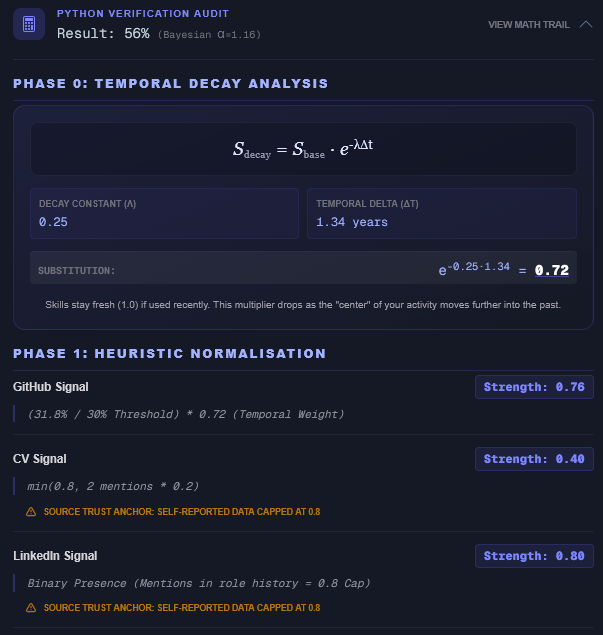
\includegraphics[width=0.85\textwidth]{implementation/screenshots/math_trail_phase_0_1.png}
    \caption{Phase 0 and Phase 1 of the Verification Audit for the a Python metric (extensible metric derived from a JD). 
    The math trail explicitly shows the application of the temporal decay penalty 
    and the heuristic normalisation of signals from the candidate's GitHub, CV, and LinkedIn.}
    \label{fig:audit_trail_phase_1}
\end{figure}

\begin{figure}[htpb]
    \centering
    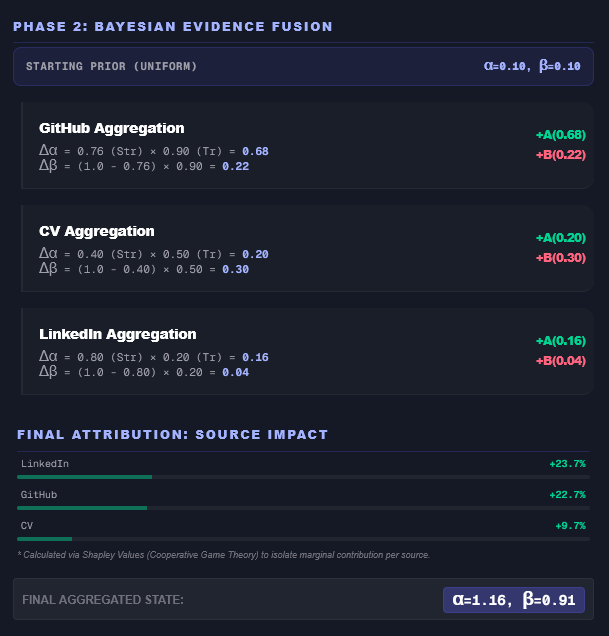
\includegraphics[width=0.85\textwidth]{implementation/screenshots/math_trail_phase_2.png}
    \caption{Phase 2 of the Verification Audit, visualising the Bayesian Evidence Fusion 
    process. It also displays the final attribution of source impact for this specific metric, 
    calculated via Shapley Values.}
    \label{fig:audit_trail_phase_2}
\end{figure}

\begin{figure}[htpb]
    \centering
    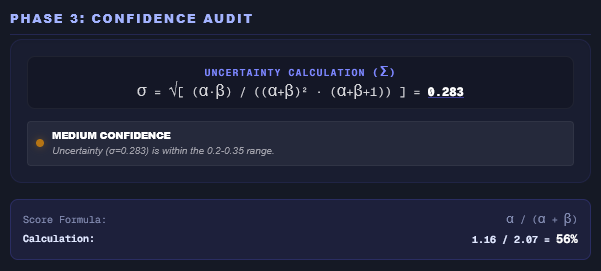
\includegraphics[width=0.85\textwidth]{implementation/screenshots/math_trail_phase_3.png}
    \caption{Phase 3 of the Verification Audit, where the mathematical uncertainty ($\sigma$) 
    of the Beta distribution is calculated to derive the final confidence level of the metric's score.}
    \label{fig:audit_trail_phase_3}
\end{figure}

\chapter{Rank Displacement Trajectories (Study 01A, 01B)}
\label{appendix:rank_displacement}

This appendix displays the graphic representations of candidate ranks among the four scoring configurations
(Traditional ATS, Modern AI ATS, CV-Only MERIT, and Full MERIT). This is for the 10-candidate cohort that we evaluate in
study 01.



\begin{figure}[htbp]
    \centering
    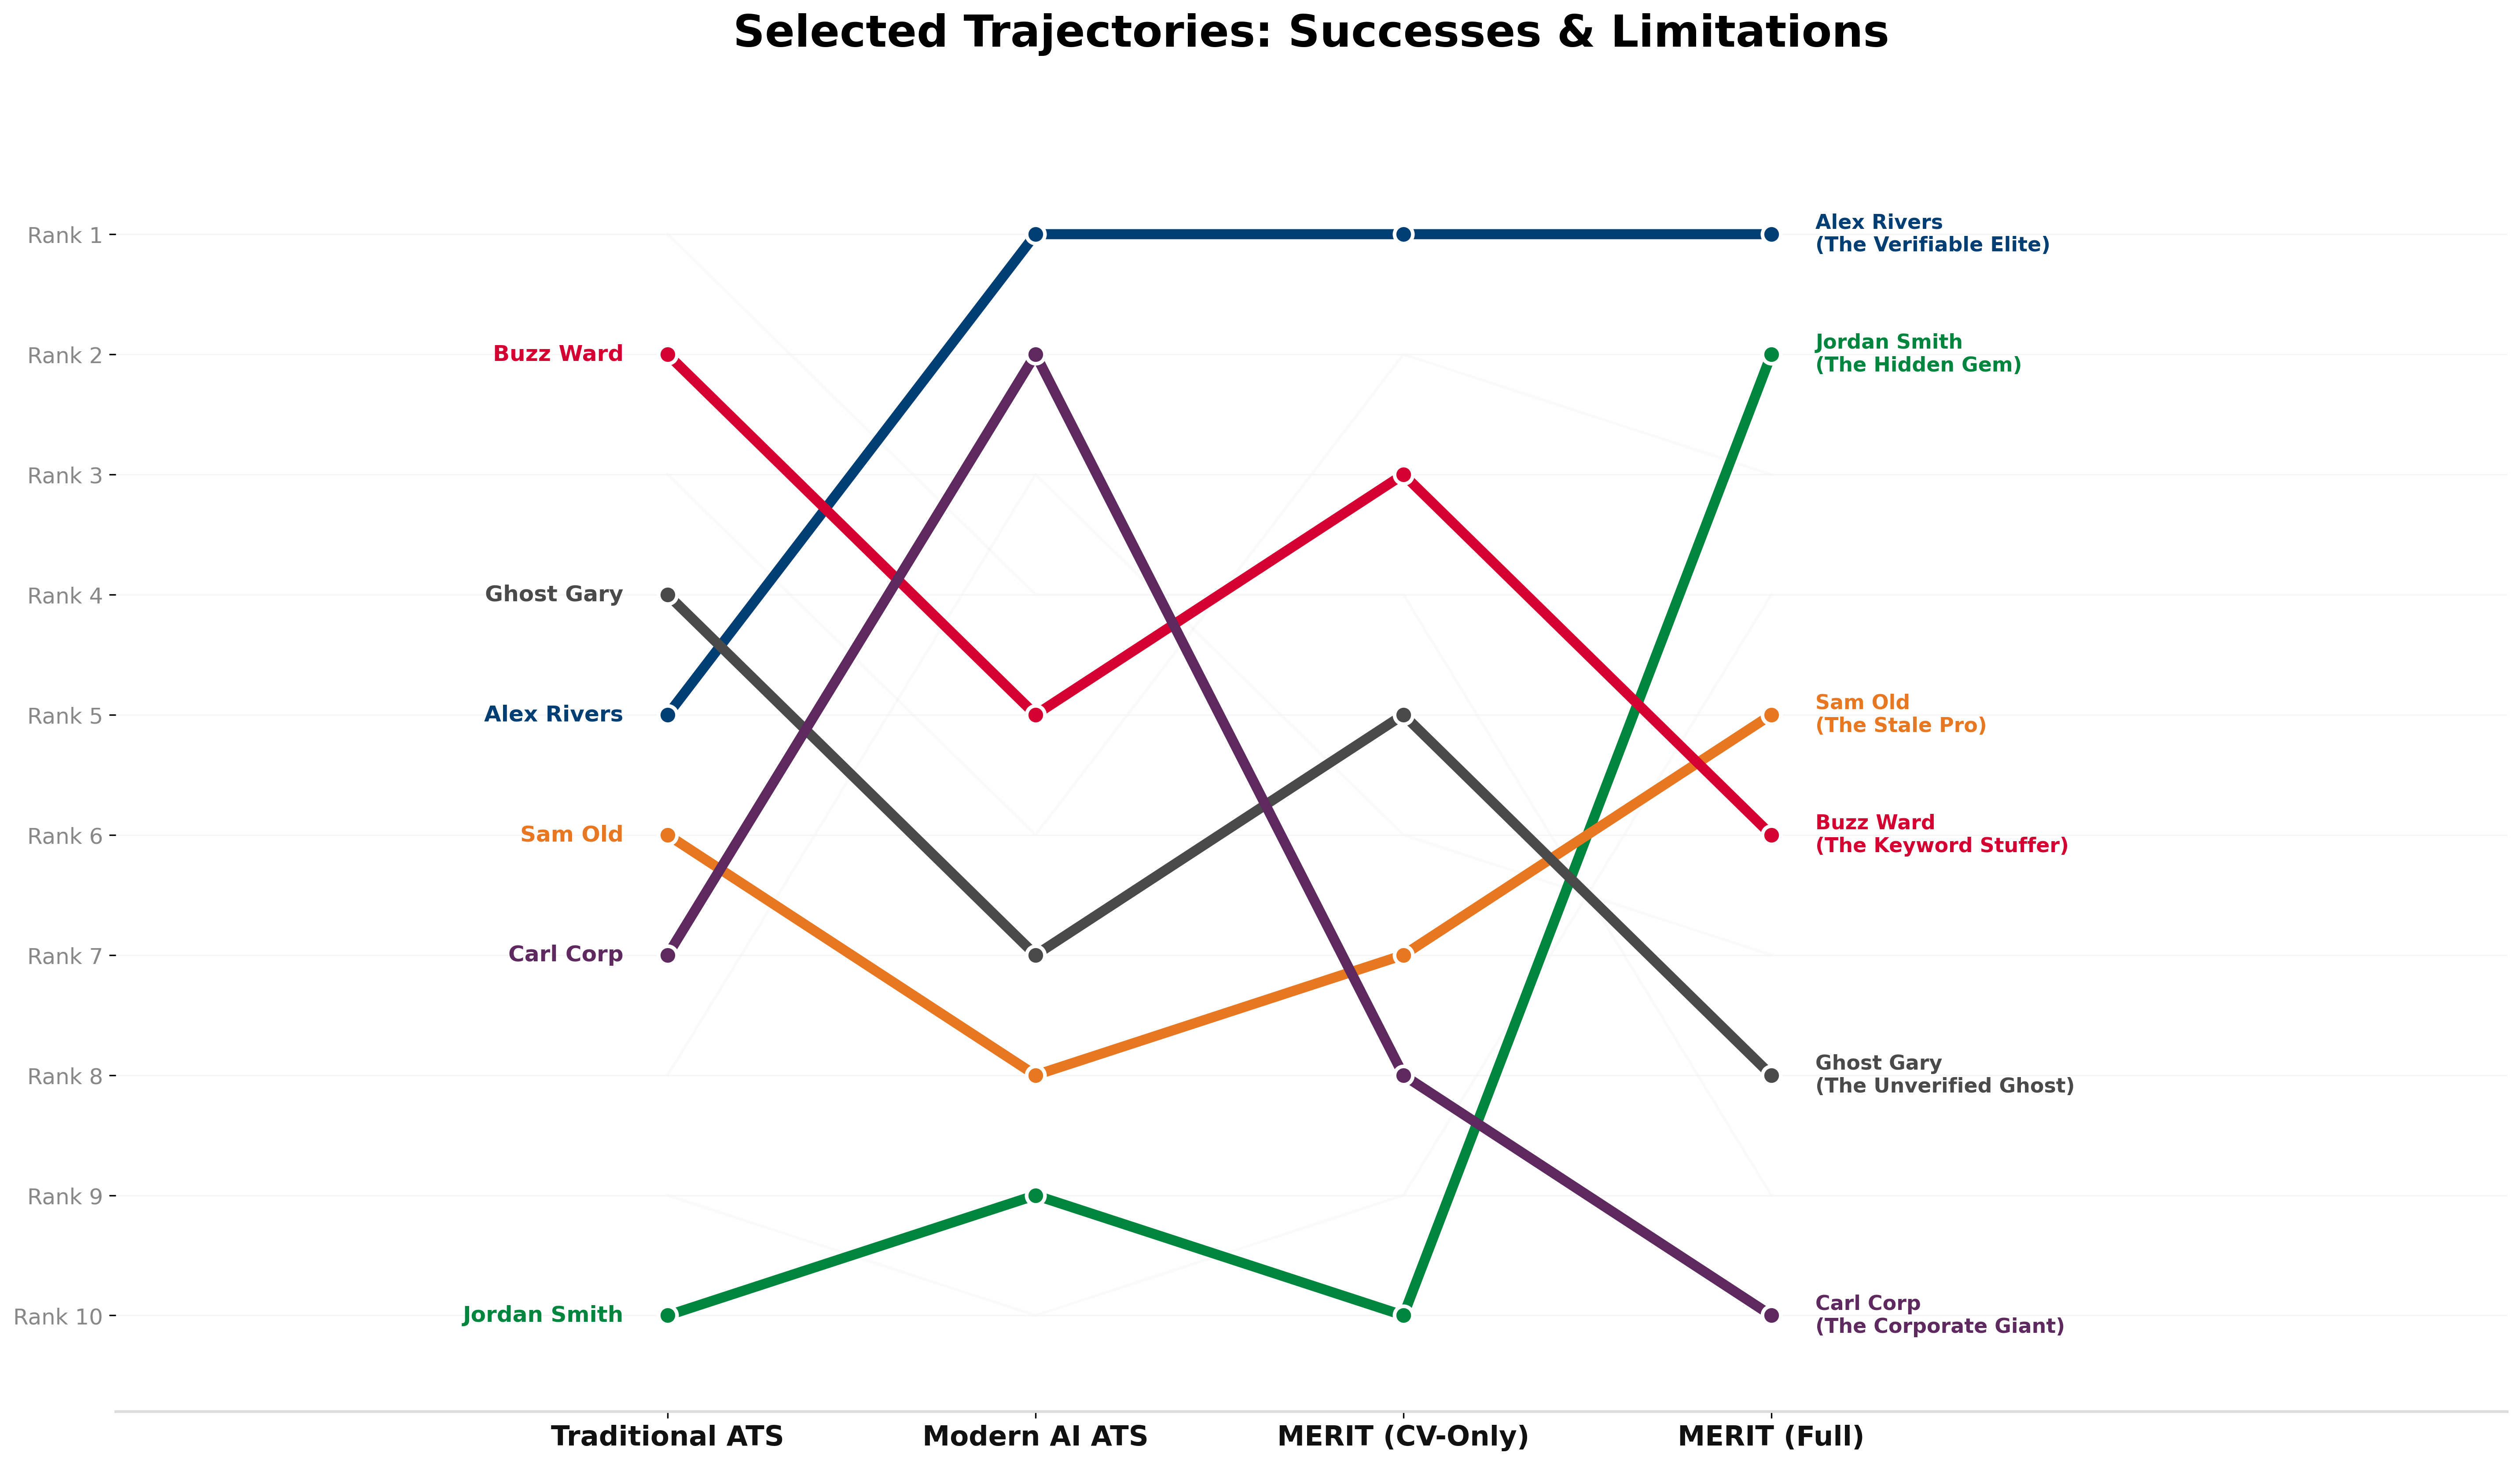
\includegraphics[width=0.95\textwidth]{../evaluation/01-comparative_study/output/rank_displacement_successes.png}
    \caption[Study~01A: Selected rank trajectories]{Study~01A: selected rank trajectories for the key candidates
    of the 10 candidate cohort. We highlight the candidates that are discussed the most in Section~\ref{subsec:study-01a-algorithmic-ablation}
    for better visual clarity. The scores are tabulated in Table~\ref{tab:algorithmic-ablation}.}
    \label{fig:rank-displacement-successes}
\end{figure}

\begin{figure}[htbp]
    \centering
    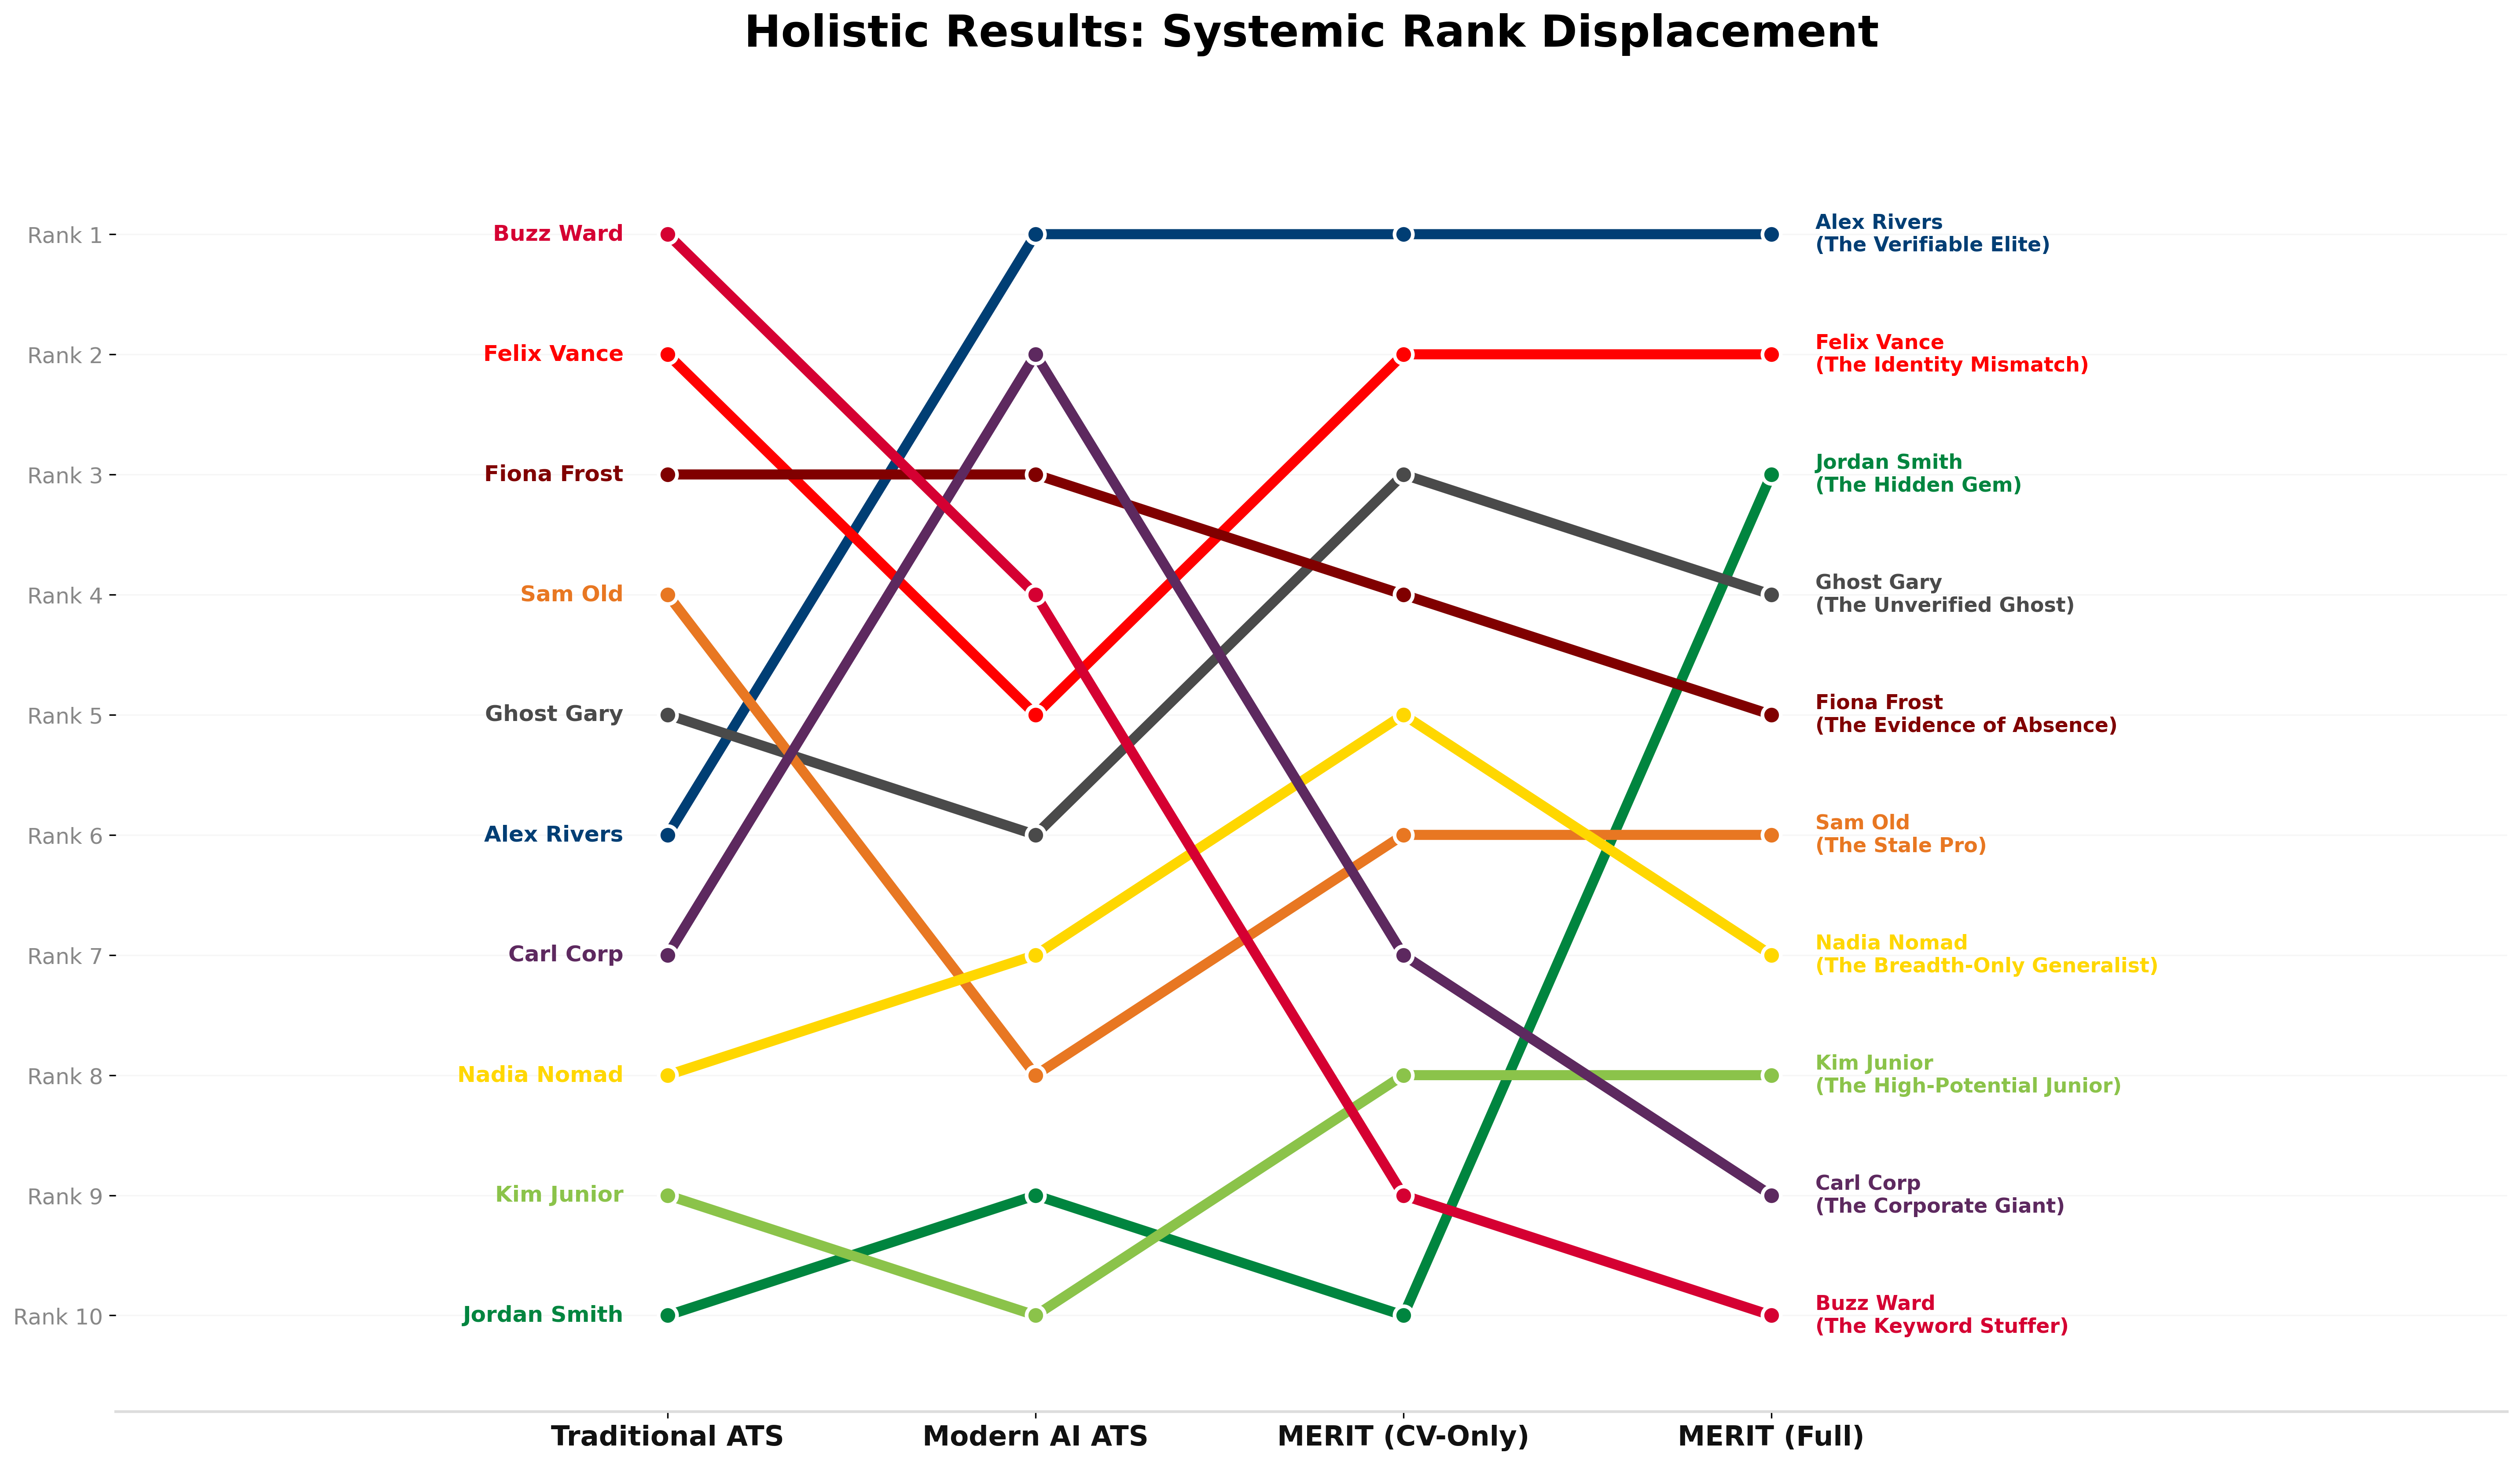
\includegraphics[width=0.92\textwidth]{../evaluation/01-comparative_study/output/rank_displacement_holistic.png}
    \caption[Study~01A: Full rank displacement]{Study~01A: full rank displacement across all ten candidate personas.
    This chart is provided for completeness, refer to Figure~\ref{fig:rank-displacement-successes} 
    for the selected rank trajectories.}
    \label{fig:rank-displacement-holistic}
\end{figure}


\bibliographystyle{vancouver}
\bibliography{bibs/introduction,bibs/background,bibs/implementation}


\chapter{Declarations}

\section{Use of Generative AI}

Generative AI tools were used in this project to assist with routine coding tasks, debugging, frontend development, styling, and the creation of test cases. 
The tools used include ChatGPT, VS Code Copilot, and Cursor. 
In all cases, any code produced by these systems was carefully reviewed and modified where necessary to ensure alignment with MERIT's requirements and quality standards. 
No AI-generated material was used for the core algorithm design, including the scoring logic and conceptual framework. 
All final submissions reflect the author's independent work and understanding.

\section{Ethical Considerations}

This project involved processing sensitive data from candidate CVs, LinkedIn profiles, and GitHub repositories. 
Ethical issues such as privacy, consent, and bias were carefully considered. 
Most candidate data used during testing was anonymised or synthetic to prevent disclosure of personal information.
For live LinkedIn ingestion tests, at most 50 profiles were retrieved via Apify; each belonged to a personal contact who gave informed consent for FYP use only (see Chapter~6). This approach is not intended for deployment.
In cases where anonymisation was not possible, data was stored securely using a reliable database provider such as Firebase. 
Ethical reviews were conducted with the project supervisor to ensure compliance with relevant guidance, and no formal ethics approval was required given the limited scale, consent-based live subset, and predominant use of synthetic or anonymised evaluation data.

\section{Sustainability}

The project does not pose any significant environmental impacts. 
MERIT operates as a lightweight software system, and its development and deployment are not expected to contribute meaningfully to carbon emissions or resource consumption.

\section{Availability of Data and Materials}

All project source code, test cases, and supporting scripts are available within the project repository: \textit{[TODO: add link]}. 
Synthetic datasets used for testing and demonstration are included in the repository. No sensitive or personally identifiable information has been shared. 
Full access is provided to allow replication, evaluation, and verification of results.

\end{document}